\documentclass[10pt]{article}
\usepackage[a4paper,top=2cm,bottom=4cm,left=2.5cm,right=2.5cm]{geometry}
\usepackage[export]{adjustbox}
\usepackage[utf8]{inputenc}
\usepackage[T1]{fontenc}
\usepackage{graphicx}
\usepackage{titlepic}
\usepackage{bbm}
\usepackage{mathtools}
\usepackage{amsmath}
\usepackage{amssymb}
\usepackage{amsthm}
\usepackage{ulem}
\usepackage{amsfonts}
\usepackage{accents}
\usepackage{subcaption}
\usepackage{multicol}
\usepackage{hyperref}
\usepackage{enumitem}
\usepackage{mathtools}
\setlist[itemize]{label=\textbullet}
\linespread{1.3}
\newcommand{\ubar}[1]{\underaccent{\bar}{#1}}

\theoremstyle{plain} 
\def\Xint#1{\mathchoice 
  {\XXint\displaystyle\textstyle{#1}}% 
  {\XXint\textstyle\scriptstyle{#1}}% 
  {\XXint\scriptstyle\scriptscriptstyle{#1}}% 
  {\XXint\scriptscriptstyle\scriptscriptstyle{#1}}% 
  \!\int} 
\def\XXint#1#2#3{{\setbox0=\hbox{$#1{#2#3}{\int}$} 
  \vcenter{\hbox{$#2#3$}}\kern-.5\wd0}} 
\def\dashint{\Xint-}

\newtheorem{thm}{Teorema}[section] 
\newtheorem{cor}[thm]{Corollario} 
\newtheorem{lem}[thm]{Lemma} 
\newtheorem{prop}[thm]{Proposizione} 
\theoremstyle{definition}
\newtheorem{defn}{Definizione}
\newtheorem{oss}{Osservazione} 

\title{Appunti Analisi III}

\author{\\
		\\  
        Garbi Luca, Libardi Gabriele\\
        \\   
}
\date{{\LARGE Primo semestre a.a. 2018/2019\footnote{Sono riportate le note delle lezioni della sola prima parte del corso (fino alla lezione del 16 Novembre), quelle sulla seconda parte, ovvero sulle \textit{forme differenziali}, sono ancora da trascrivere.}}}


\begin{document}

\maketitle 

\thispagestyle{empty} %rimuove numero pg
\newpage 
\tableofcontents
\newpage

\section{Lezione del 14 Settembre 2018}
\subsection{Integrazione per funzioni a una variabile}
Come è noto dai corsi di Analisi precedente è possibile interpretare l'integrale di una funzione come l'area della regione sottesa al grafico della funzione,

\begin{minipage}{.6\textwidth}
 dove conteremo con un contributo positivo l'area per valori positivi dell'ordinata (B in figura), mentre l'area per valori negativi della $y$ (A in figura) avrà un contributo negativo. Il procedimento per calcolare quest'area consiste nel suddividere l'intervallo $[a, b]$ nel quale si vuole calcolare l'integrale in sotto intervalli.
\end{minipage}%
\begin{minipage}{.50\textwidth}
\centering
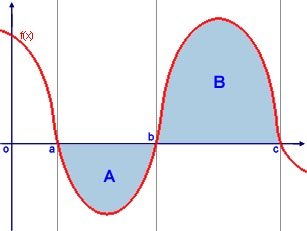
\includegraphics[width=.9\textwidth]{fig1.jpg}
\end{minipage}
Chiameremo $\mathcal{P}$ una partizione dell'intervallo $[a, b]$: $a=x_0<x_1<...<x_k=b$; $[a, b]$ sarà quindi diviso in intervalli del tipo $[x_{j-1},x_j]$ con $j=1,...,k$. 
A questo punto possiamo introdurre le \textbf{somme di Darboux}:
\begin{itemize}
    \item somma inferiore di Darboux (s in figura): $I_*(f,\mathcal{P})=\sum_{j=1}^km_j(x_j-x_{j-1})$ 
    \\ con $m_j=\inf\{ f(x): x\in [x_{j-1},x_j]\}$;
    \item somma superiore di Darboux (S in figura): $I^*(f,\mathcal{P})=\sum_{j=1}^kM_j(x_j-x_{j-1})$ 
    \\ con $M_j=\sup\{ f(x): x\in [x_{j-1},x_j]\}$.
\end{itemize}

\begin{figure}[ht]
\centering
\centerline{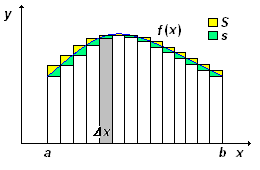
\includegraphics[width=75 mm,scale=1]{fig2.png}}
\label{fig: }
\end{figure}


\bigskip La definizione di integrabilità secondo Riemann (che si può dimostrare essere conseguenza di quella secondo Darboux) a due dimensioni è la seguente:
\\ \textit{\textbf{Definizione:} Sia $f:[a,b]\to \mathbb{R}$ limitata. Diremo che $f$ è integrabile (secondo Riemann) se esiste ed è unico $I\in \mathbb{R}$ tale che:
\begin{equation*}
    I_*(f,\mathcal{P})\leq I \leq I^*(f,\mathcal{P}), \forall \mathcal{P}.
\end{equation*}
}

\subsection{Integrazione per funzioni a due variabili}
\bigskip Possiamo passare ora alla rappresentazione grafica di integrale anche di \textbf{funzioni a due variabili}. \\ \\
\begin{minipage}{.6\textwidth}
In questo caso quello che prima era un intervallo di $\mathbb{R}$, ora è un rettangolo che chiameremo $R$, quindi andremo a studiare il volume della regione sottesa al grafico di $f:[a,b]\times[c,d]\to \mathbb{R}$. Di nuovo suddividiamo il dominio di questa $f$ in sotto domini $\{R_{ij}\}$ dati da una partizione $\mathcal{P}$:
\end{minipage}%
\begin{minipage}{.50\textwidth}
\centering
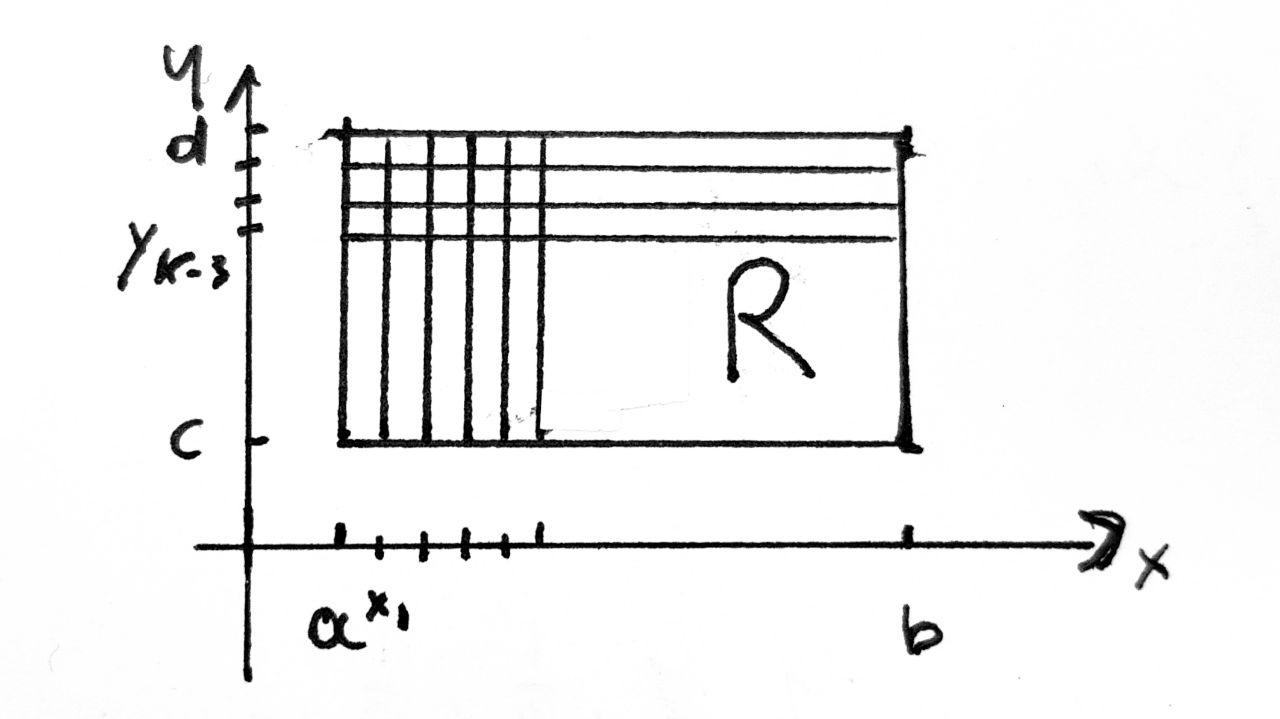
\includegraphics[width=.9\textwidth]{fig3.jpg}
\end{minipage}
\begin{equation*}
    [a,b]=\bigcup_{i=1}^h[x_{i-1},x_i]; \quad [c,d]=\bigcup_{j=1}^l[y_{j-1},x_j].
\end{equation*}
Analogamente al caso bidimensionale definiamo le somme di Darboux come:
\begin{itemize}
    \item somma inferiore di Darboux: $I_*(f,\mathcal{P})=\sum_{i,j}m_{ij}\mathcal{A}(R_{ij})$ 
    \\ con $m_{ij}=\inf\{ f(x,y): (x,y)\in R_{ij}\}$, dove $\mathcal{A}()$ indica l'area;
    \item somma superiore di Darboux: $I^*(f,\mathcal{P})=\sum_{i,j}M_{ij}\mathcal{A}(R_{ij})$ 
    \\ con $M_{ij}=\sup\{ f(x,y): (x,y)\in R_{ij}\}$, dove $\mathcal{A}()$ indica l'area.
\end{itemize}

\begin{figure}[ht]
\centering
\centerline{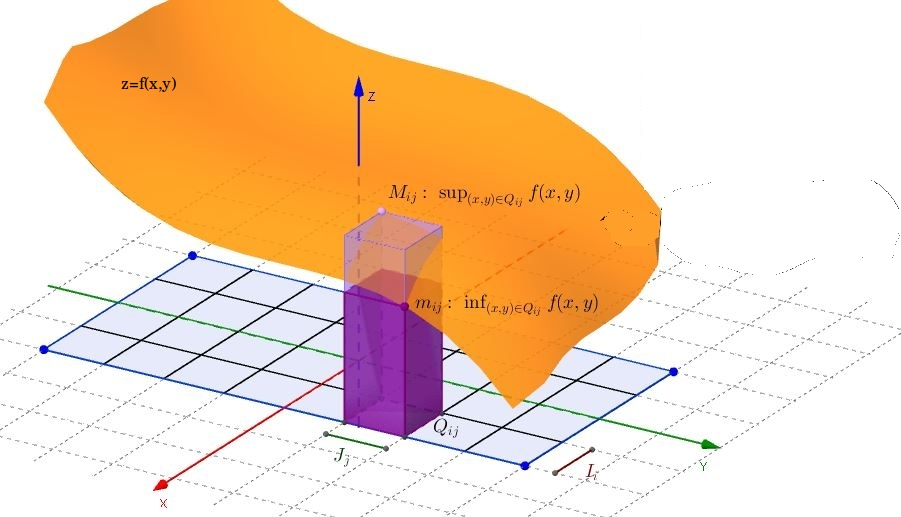
\includegraphics[width=93 mm,scale=1]{fig4.jpg}}
\label{fig: }
\end{figure}

\textit{\textbf{Definizione:} Sia $f:R\to \mathbb{R}$ limitata. Diremo che $f$ è integrabile in $R$ (secondo Riemann) se esiste ed è unico $I\in \mathbb{R}$ tale che
\begin{equation*}
    I_*(f,\mathcal{P})\leq I \leq I^*(f,\mathcal{P}), \forall \mathcal{P}.
\end{equation*}
}
Scriveremo allora $I=\int_Rf=\int_RfdA$.
\subsection{Esempi di integrazione per funzioni a due variabili}
\subsubsection{Esempio 0}
$f(x,y)=k \in \mathbb{R}, (x,y) \in R.\ \mathbb{P}$ partizione di $R$.\\ Si ha che $m_{ij}=k=M_{ij}$ e $ i=1,...,h,\ j=1,...,l$. Allora 
\begin{equation*}
    I_*(f,\mathcal{P})=I^*(f,\mathcal{P})=\sum_{i,j}k\mathcal{A}(R_{ij})=k\sum_{i,j}\mathcal{A}(R_{ij})=k\mathcal{A}(R)
\end{equation*}

\
\begin{minipage}{.5\textwidth}
\end{minipage}%
\begin{minipage}{.50\textwidth}
\centering
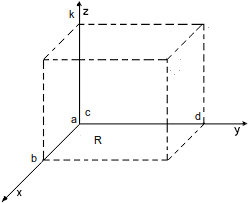
\includegraphics[width=.9\textwidth]{fig5.png}
\end{minipage}
\\

\subsubsection{Esempio 1}
Prendiamo $R=[0,1]\times [0,1]$, si può poi adattare per traslazioni e dilatazioni.
\begin{equation}
  f(x,y)=
   \begin{cases}
   1\qquad x=y=0\\0 \qquad altrove
   \end{cases}
\end{equation}
Fuori dall'origine $\forall \mathcal{P}$ abbiamo che le somme superiori e quelle inferiori sono nulle. Per $R_{11}$ invece solo le somme inferiori sono nulle, quelle superiori sono pari ad $\mathcal{A}(R_{11})$. Per definizione abbiamo bisogno di un $I$ reale tale che $0\leq I\leq \mathcal{A}(R_{ij})$ per qualsiasi scelta di $\mathcal{P}$, l'unico valore possibile è $I=0$.


\subsubsection{Esempio 2} \label{notint}
$R=[0,1]\times [0,1]$.
\begin{equation}
  f(x,y)=
   \begin{cases}
   1\qquad x,y \in \mathbb{Q}\cap [0,1]\\0 \qquad altrove\ (in\ \mathbb{R})
   \end{cases}
\end{equation}
Presa una  partizione $\mathcal{P}$ ($R_{i,j}=[x_{i-1},x_i]\times [y_{j-1},y_j]$), all'interno di ogni intervallo sia per la $x$ che per la $y$ troviamo infiniti razionali poiché sono densi. Quindi per ogni scelta di $\mathcal{P}$ vale $I_*(f,\mathcal{P})=0$ e $I^*(f,\mathcal{P})=\sum_{i,j}1\cdot \mathcal{A}(R_{ij})= \mathcal{A}(R)=1$.
\\ Ma poiché NON esiste un unico $I$ reale tale che $0\leq I\leq1$ per qualsiasi partizione, concludiamo che $f$ non è integrabile secondo Riemann.

\subsubsection{Esempio 3}
$R=[0,1]\times [0,1]$.
\begin{equation}
  f(x,y)=
   \begin{cases}
   1\qquad x=0, y \in \mathbb{Q}\cap [0,1]\\0 \qquad altrove
   \end{cases}
\end{equation}
Per ogni scelta della partizione $\mathcal{P}$ vale $I_*(f,\mathcal{P})=0$. Notiamo che anche tutti i $M_{ij}$ per $i\neq 1$ sono nulli, quindi l'unico contributo alle somme superiori è dato dalla somma dei rettangoli di base $x_1$: $I^*(f,\mathcal{P})=\sum_{i,j}1\cdot \mathcal{A}(R_{1j})= x_1\cdot 1=x_1$.
 Per definizione abbiamo bisogno di un $I$ reale tale che $0\leq I\leq x_1$ per qualsiasi scelta di $\mathcal{P}$, l'unico valore possibile è $I=0$.
 
 
\subsubsection{Esempio 3.bis}
Esercizio per casa: studiare l'integrabilità della seguente funzione in
$R=[0,1]\times [0,1]$:
\begin{equation}
  f(x,y)=
   \begin{cases}
   1\qquad x\in \{ \alpha_1,...,\alpha_n\}, n<\infty \in \mathbb{N}, y \in \mathbb{Q}\cap [0,1]\\0 \qquad altrove
   \end{cases}
\end{equation}

\subsubsection{Esempio 4}
$R=[0,1]\times [0,1]$.
\begin{equation}
  f(x,y)=
   \begin{cases}
   1\qquad x=y=1,\frac{1}{2},\frac{1}{3}, ...\\0 \qquad altrove
   \end{cases}
\end{equation}

\begin{figure}[ht]
\centering
\centerline{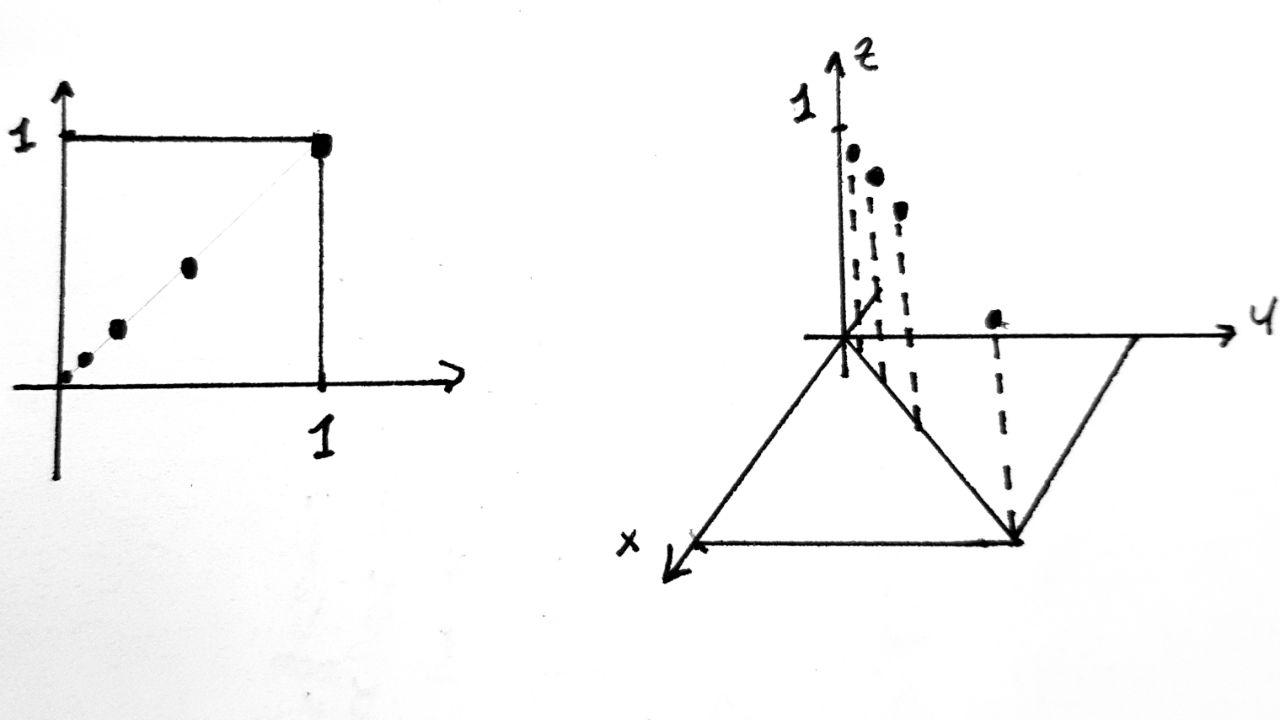
\includegraphics[width=93 mm,scale=1]{fig6.jpg}}
\label{fig: }
\end{figure}

Come nel caso ad una variabile vale che date due funzioni $f,g;R\to \mathbb{R}$ integrabili e $f\leq g$ in $R\Rightarrow \int_Rf\leq \int_Rg$. 
\\ Studiamo allora la funzione 
\begin{equation}
  g(x,y)=
   \begin{cases}
   1\qquad x=y\\0 \qquad altrove
   \end{cases}
\end{equation}
che in $R$ è sempre maggiore o uguale a $f$. Prendiamo una partizione uniforme di $R$, ovvero tale che $x_i-x_{i-1}=y_j-y_{j-1}=k$ con $k$ costante $\forall i,j$. Quindi $R$ sarà suddiviso in quadratini della stessa area. Risulta evidente che per questo tipo di partizione, essendo $R$ un quadrato, deve essere che il numero di sottointervalli dell'ordinata debba essere pari a quelli dell'ascissa, chiamiamo questo numero $N$ (avremo $k=1/N^2$). Le somme inferiori sono nulle, per il calcolo di quelle superiori invece possiamo contare per quanti quadratini passa la retta $x=y$: sono $N$ sulla diagonale principale, più quelli di cui viene toccato un vertice sulla sopradiagonale ($N-1$) e sottodiagonale ($N-1$), il totale è $3N-2$. In questi quadratini si ha $M_{ij}=1$, per cui $$I^*(f,\mathcal{P})=1\cdot (3N-2)\cdot \frac{1}{N^2}=\frac{3}{N}-\frac{2}{N^2}.$$ 
 Per definizione abbiamo bisogno di un $I$ reale tale che $0\leq I\leq \frac{3}{N}-\frac{2}{N^2} \leq \frac{3}{N}$ per qualsiasi scelta di $\mathcal{P}$. L'unico valore possibile per la partizione scelta è $I=0$, ma non so cosa succeda scegliendo altre partizioni.
 
 \section{Lezione del 19 Settembre 2018}
 \subsection{Criterio di integrabilità}
 Vediamo due lemmi che ci serviranno per dimostrare il criterio di Riemann di integrabilità di una funzione.
\begin{lem}
 $R\subset \mathbb{R}^2$ rettangolo compatto, non vuoto e non degenere. $\mathcal{P}$ partizione di $R$, $f:R\to \mathbb{R}$ limitata allora vale $$I_*(f,\mathcal{P})\leq I^*(f,\mathcal{P}).$$
\end{lem}
La dimostrazione è semplice e ovvia.
\begin{lem}
 $R\subset \mathbb{R}^2$ rettangolo compatto, non vuoto e non degenere. $\mathcal{P}_1, \mathcal{P}_2$ partizioni di $R$, $f:R\to \mathbb{R}$ limitata allora vale $$I_*(f,\mathcal{P}_1)\leq I^*(f,\mathcal{P}_2).$$
 \label{lem: somme sup somme inf}
\end{lem}
\begin{proof}
Diamo la definizione di \textit{raffinamento} utile per la dimostrazione.
Diremo che la partizione $\mathcal{P}'$ è raffinamento della partizione $\mathcal{P}$ se ogni sottorettangolo in  $\mathcal{P}'$ è contenuto in un sottorettangolo di $\mathcal{P}$. 
\\ Ora, date le 2 partizioni $\mathcal{P}_1 = \left \{R_i^{(1)} \right \}$,  $\mathcal{P}_2 =  \left \{R_j^{(2)} \right \}$ di $R$, possiamo trovare un raffinamento comune di entrambe che chiamo $\mathcal{P}$ =  $\mathcal{P}_1 \vee  \mathcal{P}_2 =  \left \{R_k \right \}$. A questo punto notiamo che $$R_k\subseteq R_i^{(1)}\Rightarrow \inf f(R_i^{(1)})\leq \inf f(R_k) $$
 e che
 $$R_k\subseteq R_j^{(2)}\Rightarrow \sup f(R_k)\leq \inf f(R_j^{(2)}). $$
 Ma per il lemma precedente $$I_*(f,\mathcal{P}_1)\leq I_*(f,\mathcal{P})\leq I^*(f,\mathcal{P}) \leq I^*(f,\mathcal{P}_2).$$
\end{proof} 
\begin{thm} (Criterio di Riemann) Sia $f:R\to \mathbb{R}$ limitata, la funzione $f$ è integrabile su $R$ $\Leftrightarrow \forall \ \varepsilon \! \! >\! \! 0\ \exists \ \mathcal{P}$ tale che $$I^*(f,\mathcal{P})-I_*(f,\mathcal{P})<\varepsilon$$.
  \end{thm}
 \begin{proof} \
 \newline
 \textbf{($\Leftarrow$)} Supponiamo \textit{per assurdo} che $f$ non sia integrabile, allora non esiste un unico $I$ reale tale che $I_*(f,\mathcal{P})\leq I \leq I^*(f,\mathcal{P})$, ma esisterà un intervallino di estremi $I_1$ e $I_2$ di valori che soddisfano la disuguaglianza. Poniamo $I_1<I_2$ e definisco $\Bar{\varepsilon}=I_2-I_1>0$. Allora abbiamo
 $$ I^*(f,\mathcal{P})- I_*(f,\mathcal{P})\geq \Bar{\varepsilon}.$$ Di conseguenza possiamo scegliere $\epsilon=\varepsilon$, e per la partizione $\mathcal{P}$ non è soddisfatta $I^*(f,\mathcal{P})-I_*(f,\mathcal{P})<\varepsilon$, ciò contraddice l'ipotesi. Dobbiamo concludere quindi che $f$ sia integrabile.
\newline
 \textbf{($\Rightarrow$)} Assumo che esista un unico $I$ reale tale che valga la definizione di integrabilità. Allora fissato un $\varepsilon >0$ esisterà una partizione $\mathcal{P}_2$ per cui $I^*(f,\mathcal{P}_2)-I<\varepsilon/2$ e una partizione $\mathcal{P}_1$ tale che $I-I_*(f,\mathcal{P}_1)<\varepsilon/2$. Chiamata allora $\mathcal{P}=\mathcal{P}_1\vee\mathcal{P}_2$, per $\mathcal{P}$ vale il lemma \ref{lem: somme sup somme inf}. Ne consegue le tesi.
 \end{proof} 
 \subsection{Proprietà ed estensione dell'integrazione}
 Elenchiamo di seguito alcune proprietà dell'integrazione. Supponiamo $R$ compatto, non vuoto, non degenere. $f,g:R\to\mathbb{R}$ integrabili, $\alpha \in \mathbb{R}$, allora 
 \begin{enumerate}
     \item $f+g$ è integrabile e vale $$\int_R(f+g)dV_n=\int_RfdV_n+\int_RgdV_n;$$
     \item $\alpha f$ è integrabile e vale 
     $$\int_R \alpha fdV_n=\alpha \int_RfdV_n;$$
     \item Se separo in $R$ in due sottorettangoli $R'$ e $R''$ $\Rightarrow f$ è integrabile in $R'$ e $R''$  e vale
      $$\int_R fdV_n=\int_{R'}fdV_n+\int_{R''}fdV_n.$$
 \end{enumerate}
 Ricordiamo ora la definizione di continuità uniforme.
 \begin{defn}
 Diremo che $f:R\to\mathbb{R}$ è uniformemente continua se per ogni $\varepsilon>0\ \exists \ \delta(\varepsilon)$ tale che $\forall \vec{x}, \vec{y} \in R$ vale se $||\vec{x}-\vec{y}||<\delta (\varepsilon)$ allora $|f(\vec{x})-f(\vec{y})|<\varepsilon$.
 \end{defn}
 Ricordiamo inoltre che per il teorema in Cantor-Heine se abbiamo una funzione continua definita su un compatto, allora la funzione è anche uniformemente continua. Vale pertanto il seguente teorema.
 \begin{thm}
   Se $f:R\to\mathbb{R}$ è continua su $R$ compatto, allora è integrabile.
 \end{thm}
\begin{proof}
Sappiamo che $f$ è uniformemente continua. Divido $R$ con una partizione $\mathcal{P}= \{ R_{ij} \}$ in modo tale che per ogni scelta degli indici $i,j$ valga $diam(R_{ij})< \delta$. Per il teorema di Weierstrass so che ogni sottorettangolo $R_{ij}$ ammette estremo superiore ($\sup f(R_{ij})=M_{ij}$) e inferiore ($\inf f(R_{ij})=m_{ij}$). Per la continuità uniforme $\varepsilon > M_{ij}-m_{ij}\geq 0$. Allora fissato $\varepsilon’=\varepsilon/\mathcal{A}(R_{ij})$ otteniamo che 
$$I^*(f, \mathcal{P})- I_*(f, \mathcal{P})=\sum_{ij}(M_{ij}-m_{ij})\mathcal{A}(R_{ij})<\sum_{ij}\varepsilon’\mathcal{A}(R_{ij})=\varepsilon$$. Per il criterio di Riemann concludiamo quindi che la funzione è integrabile.        
\end{proof}

Talvolta c'è la necessità di integrare una funzione in una regione più complicata di un rettangolo. Supponiamo ad esempio di voler calcolare l'integrale di una funzione $f$ in $\Omega \subset \mathbb{R}^2$, compatto qualsiasi. Trovandoci in $\mathbb{R}^2$, $\Omega$ è chiuso e limitato, pertanto sta in una palla chiusa di raggio finito, che a sua volta può essere circoscritta in un rettangolo $R$. Definisco allora l'estensione di $f$:
\begin{equation}
  \bar{f}(\vec{x})=
   \begin{cases}
   f(\vec{x})\qquad \ per \ \vec{x} \in \Omega \\0 \qquad \ per \ \vec{x} \in R\setminus \Omega
   \end{cases}
\end{equation}
Data questa definizione segue automaticamente che
$$\int_\Omega fd\mathcal{A} = \int_R \bar{f}d\mathcal{A},$$
a patto che sia $f$ che $\bar{f}$ siano integrabili.

\subsubsection{Esempio 1} \label{misnonnulla}
$\Omega ^2 \cap [0, 1]^2,\ f:\Omega \ni \bar{x} \mapsto 1\in\mathbb{R}.$ In questo caso $R=[0, 1]^2$ e {}
\begin{equation}
  \bar{f}(\vec{x})=
   \begin{cases}
   1\qquad \ per \ \vec{x}= (x_1, x_2) \in \Omega \\0 \qquad \ per \ \vec{x} \in R\setminus \Omega
   \end{cases}
\end{equation}
Come visto nell'esempio \ref{notint} la funzione estesa non è integrabile.
\\ Il fatto che non sia integrabile ha a che fare con la frontiera di $\Omega$, vedremo in seguito in che modo. Ricordiamo che la frontiera di un insieme può essere espressa come l'insieme dato sottraendo il suo interno alla chiusura. Nel nostro caso $cl(\Omega)=[0,1]^2$ e $int(\Omega)=\varnothing$ poiché comunque venga scelta una palla aperta centrata in un punto appartenente ad $\Omega$, al suo interno saranno presenti sempre punti non appartenenti ad $\Omega$. Per cui $$fr(\Omega)=cl(\Omega)\setminus int(\Omega)=[0,1]^2.$$
\newline
Vediamo ora il concetto di volume e misura nulla utile per dare una condizione di integrabilità all'estensione di una funzione su un dominio rettangolare.
Prima possiamo definire il concetto di \textit{misura di volume n-dimensionale} per i rettangoli in $\mathbb{R}^n$.
\begin{defn}
Posto $lungh(I)=\sup (I)-\inf (I)$.
Se $R = I_1\times I_2 \times ... \times I_n$ è un rettangolo n-dimensionale, dove $I_j$ appartiene a $\mathbb{R}$, poniamo $$vol_n(R)= lungh(I_1)\cdot lungh(I_2)\cdot ...\cdot lungh(I_n) = \prod_{j=1}^nlungh(I_j).$$
\end{defn}
\begin{defn}
$X\subset \mathbb{R}^n.$ Diremo che $X$ ha \textbf{volume nullo} se $\forall \varepsilon>0$ trovo un ricoprimento con un numero finito di rettangoli compatti $R_1, ..., R_N$ con $N\in \mathbb{N}$, per cui 
$$\sum_{i=1}^Nvol_n(R_i)<\varepsilon.$$
\end{defn}
\begin{defn}
$X\subset \mathbb{R}^n.$ Diremo che $X$ ha \textbf{misura nulla} se $\forall \varepsilon>0$ trovo un ricoprimento con un numero (anche infinito ma \textit{numerabile}) di rettangoli compatti $\{ R_i\}$ con $i\in \mathbb{N}$, per cui 
$$\sum_{i\in \mathbb{N}}^Nvol_n(R_i)<\varepsilon.$$
\end{defn}
Facciamo ora alcune osservazioni:
\begin{enumerate}
    \item Notiamo che per come sono stati definiti questi concetti, se un insieme ha volume nullo, questo implica che anche la sua misura lo sia, ma non vale il contrario.
    \item Si può vedere che $\Omega = [0,1]^2\cap \mathbb{Q}^2$ è un insieme a misura nulla.
    \item Un semplice segmento ha volume bidimensionale (in $\mathbb{R}^2$) nullo, ma in $\mathbb{R}$ no.
    \item Ogni aperto limitato in $\mathbb{R}^n$ ha volume n-dimensionale sempre maggiore di 0.
\end{enumerate}
\bigskip
A questo punto possiamo dare gli enunciati di due teoremi utili per dare la condizione di integrabilità della funzione estesa che stavamo cercando.
\begin{thm}
  Sia $f:R\to \mathbb{R}$ limitata. Se $f$ è continua a meno di un insieme $Z\subset R$ con volume nullo, allora $f$ è integrabile.
\end{thm}
\begin{thm}
  (di Lebesgue-Vitali)
  Sia $f:R\to \mathbb{R}$, $R \subset \mathbb{R}^n$ compatto. $f$ è integrabile $\Leftrightarrow$ $f$ è limitata e l'insieme dei punti di discontinuità di $f$ ha misura nulla.
\end{thm}
\bigskip Tornando ora all'estensione di una funzione $f$ su un rettangolo che circoscrive un compatto $\Omega$ nel quale $f$ è continua, come corollario abbiamo che l'estensione di $f$ è integrabile a patto che $fr(\Omega)$ abbia misura nulla. 

 \section{Lezione del 21 Settembre 2018}
 \subsection{Integrale iterato}
 \begin{thm}
   $f,g$ integrabili in $\Omega \subset \mathbb{R}^n$ compatto con frontiera a volume n-dimensionale nullo, allora se $f\leq g$ in $\Omega$ vale
   $$\int_\Omega fdV_n\leq \int_\Omega gdV_n.$$
 \end{thm}
\begin{proof}
$h=g-f\Rightarrow h\geq 0$ su $\Omega$. Ma allora $I_*(h,\mathcal{P})\geq 0$, quindi $I=\int_\Omega hdV_n \geq 0$. Per la linearità dell'integrale segue la tesi.
\end{proof}

\subsubsection{Esercizio 1}
 $f(x,y)=x^2 - y$ \qquad $R = [0,2] \times [1,3]$ \\
rettangolo compatto $\longrightarrow$ esiste volume finito per Weiestrass (funzione continua su un compatto)\\
$$\int_R f \, dA = \int_{y=1}^{y=3} \left( \int_{x=0}^{x=2} (x^2 - y) \,dx \right) \,dy$$
$$= \int_{1}^{3} \left[ \frac{x^3}{3} - yx\right]{x=0}^{x=2} \,dy = \int{1}^{3} \left( \frac{8}{3} -2y \right) \,dy = \left[ \frac{8}{3} y - y^2\right]_{y=1}^{y=3} = 8 - 9 - \frac{8}{3} + 1 = -\frac{8}{3}$$
in questo esempio se invertiamo l'ordine degli indici di integrazione non cambia il risultato non cambia, infatti:
$$\int_R f \, dA = \int_{x=0}^{x=2} \left( \int_{y=1}^{y=3} (x^2 - y) \,dy \right) \,dx = \int_{0}^{2} \left[ x^2y - \frac{y^2}{2}\right]_{y=1}^{y=3} \,dx$$
$$= \int_{0}^{2} \left( 3x^2 - \frac{9}{2} - x^2 + \frac{1}{2} \right) \,dx = \int_{0}^{2} (2x^2 -4) \,dx = \left[ \frac{2}{3} x^3 - 4x \right]_{x=0}^{x=2} = \frac{16}{3} - \frac{24}{3} = -\frac{8}{3}$$
\\

Che succede se ho regioni di integrazione più complicate?
\\
\subsubsection{Esercizio 2}

\begin{minipage}{.5\textwidth}
$\Omega = \{ (x,y) | x \in [0,1], \quad y \in [0,x] \}$
Costruiamo un rettangolo $R=[0,1]^2$ che contenga l'intervallo di integrazione $\Omega$ e definiamo la funzione (\textit{discontinua}):
$$\bar{f}(x,y) = \begin{cases} x^2 - y & (x,y) \in \Omega \\ 0 & altrimenti \end{cases}$$
\end{minipage}%
\begin{minipage}{.50\textwidth}
\centering
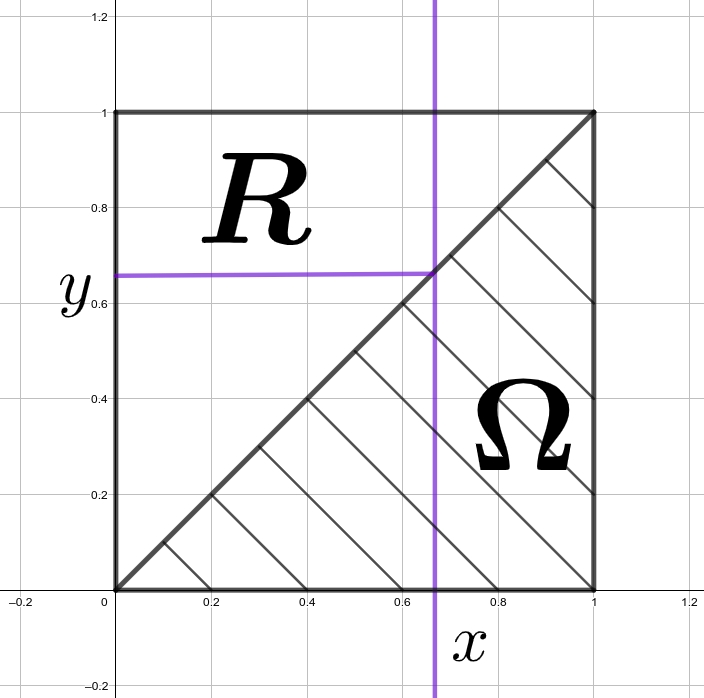
\includegraphics[width=0.8\textwidth]{fig1_libo.jpg}
\end{minipage}
\newline
Quindi l'integrale in $\Omega$ diventa un'integrale in R in questo modo:
$$\int_{\Omega} (x^2-y) \,dA = \int_{R} \bar{f} (x,y) \,dA$$
in questo esempio è più vantaggioso partire ad integrare da y perche y è in funzione di x
$$\int_0^1 \left( \int_0^1 \bar{f}(x,y)\,dy\right)\,dx$$
risolvendo singolarmente l'integrale interno
$$\int_0^1 \bar{f}(x,y)\,dy = \int_0^x (x^2-y)\,dy = \left[ x^2y-\frac{y^2}{2} \right]_{y=0}^{y=x} = x^3-\frac{x^2}{2}$$
$$\int_{\Omega} f\,dA = \int_0^1 \left( x^3 - \frac{x^2}{2}\right)\,dx = \left( \frac{x^4}{4} - \frac{x^3}{6} \right)_{x=0}^{x=1} = \frac{1}{4} - \frac{1}{6} = \frac{1}{12}$$
\\
\begin{minipage}{.5\textwidth}
Se dovessi invertire l'ordine di integrazione delle due variabili, dovrei cambiare anche l'intervallo lungo il quale integro le rispettive variabili, quindi:
$$\int_0^1 \bar{f}(x,y)\,dx = \int_y^1 (x^2 - y) \,dx =$$
$$=\left[ \frac{x^3}{3} - yx \right]_{x=y}^{x=1} = \frac{1}{3} -y -\frac{y^3}{3} +y^2$$

\bigskip
\end{minipage}%
\begin{minipage}{.50\textwidth}
\centering
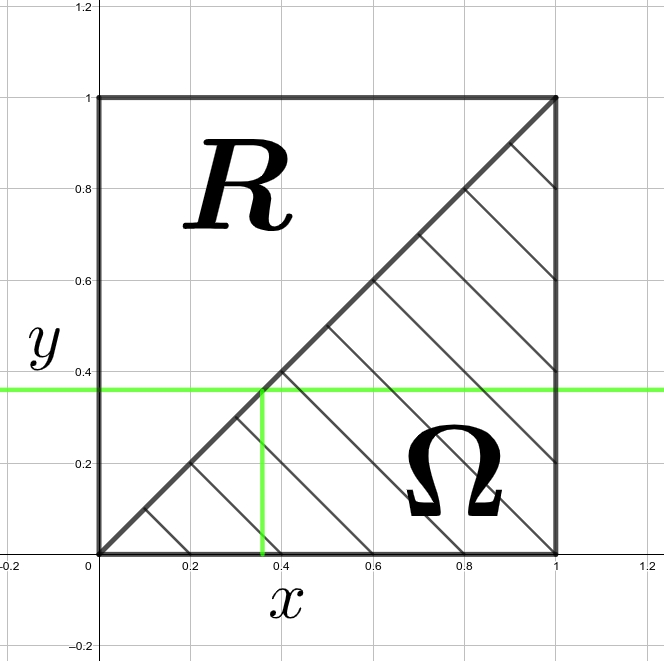
\includegraphics[width=0.8\textwidth]{fig2_libo.jpg}
\end{minipage}

E di conseguenza
$$\int_{\Omega} f\,dA = \int_0^1 \left( \frac{1}{3}-y-\frac{y^3}{3}+y^2\right)\,dy = \left[ \frac{1}{3}y - \frac{y^2}{2} -\frac{y^4}{12} + \frac{y^3}{3}\right]_{y=0}^{y=1} = \frac{1}{12}$$
\\
\subsubsection{Esercizio 3}
\begin{minipage}{.5\textwidth}
$\Omega = \{ (x,y) | x \in [0,1] \quad y \in [x,1] \}$
$$\int_0^1 \left( \int_x^1 e^{-y^2}\,dy\right)\,dx$$
L'integrale più interno non è possibile risolverlo analiticamente, quindi possiamo sfruttare il fatto che f(x,y) è continua per invertire l'ordine degli integrali.
\end{minipage}%
\begin{minipage}{.50\textwidth}
\centering
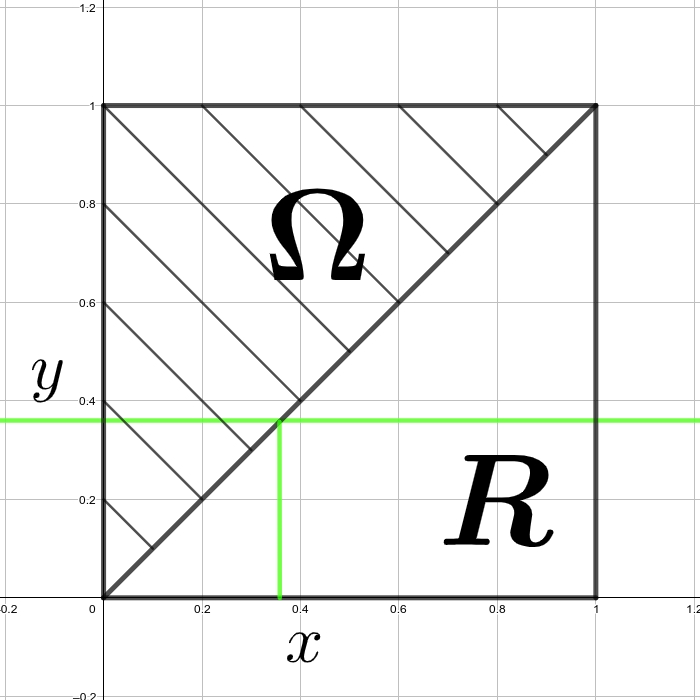
\includegraphics[width=0.8\textwidth]{fig3_libo.jpg}
\end{minipage}

$$= \int_0^1 \left( \int_0^y e^{-y^2}\,dx\right)\,dy = \int_0^1 ye^{-y^2} \,dy = \left[ -\frac{1}{2} e^{-y^2} \right]_{y=0}^{y=1} = \frac{1}{2} (1 - e^{-1})$$
\newline

\subsection{Il teorema Baby Fubini} \label{sec: babyfub}

\begin{thm} \label{th: baby_fubini}
 (Baby Fubini) Sia $f$ integrabile nel rettangolo compatto $R=[a,b]\times [c,d].$ Supponiamo che $\int_c^df(x,y)dy$ esista $\forall x\in [a,b]$ e che esista 
 $$\int_a^b \left (\int_c^d f(x,y)dy\right ) dx.$$
 Allora si ha che
 $$\int_RfdA= \int_a^b \left (\int_c^d f(x,y)dy\right ) dx.$$
 Inoltre se anche $\int_a^bf(x,y)dx$ esiste $\forall x\in [a,b]$ ed esiste anche
 $$\int_c^d \left (\int_a^b f(x,y)dx\right ) dy$$ vale che
 $$\int_RfdA= \int_c^d \left (\int_a^b f(x,y)dx\right ) dy.$$
\end{thm}

\begin{proof}
Fissiamo $\varepsilon>0$ ad arbitrio.
\\ Sia $\mathcal{P} = \{ R_{ij} \}$ una partizione di $R$, con $R_{ij}=[x_{i-1},x_i]\times[y_{j-1},y_j]$ per $i=1,...,L$ e $j=1,...,M$. Chiameremo $m_{ij}\doteq \inf(f(R_{ij}))$ e $M_{ij}\doteq \sup(f(R_{ij}))$.
Chiaramente $\forall (x,y)\in R_{ij}$, si ha $m_{ij}\leq f(x,y) \leq M_{ij}$.
Pertanto, integrando su $x \in [x_{i-1},x_i]$, si ha
$$m_{ij}(x_i-x_{i-1})\leq \int_{x_{i-1}}^{x_i} f(x,y)\ dx \leq M_{ij}(x_i-x_{i-1})$$.
Quindi
$$\sum_{i=1}^L m_{ij}(x_i-x_{i-1}) \leq \sum_{i=1}^L \int_{x_{i-1}}^{x_i} f(x,y)\ dx \leq \sum_{i=1}^L M_{ij}(x_i-x_{i-1})$$.
Cioè 
$$\sum_{i=1}^L m_{ij}(x_i-x_{i-1}) \leq \int_a^b f(x,y)\ dx \leq \sum_{i=1}^L M_{ij}(x_i-x_{i-1})$$.
Integriamo ora su $y \in [y_{j-1},j_i]$:
$$\sum_{i=1}^L m_{ij}(x_i-x_{i-1})(y_j-y_{j-1}) \leq \int_{y_{j-1}}^{y_j} \int_a^b f(x,y)\ dxdy \leq \sum_{i=1}^L M_{ij}(x_i-x_{i-1})(y_j-y_{j-1}) $$.
Allora chiaramente
$$\sum_{j=1}^M \sum_{i=1}^L m_{ij}(x_i-x_{i-1})(y_j-y_{j-1}) \leq \int_c^d \int_a^b f(x,y)\ dxdy \leq \sum_{j=1}^M  \sum_{i=1}^L M_{ij}(x_i-x_{i-1})(y_j-y_{j-1}) $$,
ovvero
$$\sum_{i,j} m_{ij} \mathcal{A}(R_{ij}) \leq \int_c^d \int_a^b f(x,y)\ dxdy \leq \sum_{i,j} M_{ij}\mathcal{A}(R_{ij})$$.
Ma vediamo che l'integrale doppio è maggiorato e minorato rispettivamente dalle somme di Darboux superiori e inferiori di $f$ per la partizione $\mathcal{P}$:
$$I_*(f, \mathcal{P}) \leq \int_c^d \int_a^b f(x,y)\ dxdy \leq I^*(f, \mathcal{P})$$.
Dato che $f$ è integrabile per ipotesi e l'integrale è unico per definizione, si conclude necessariamente che
$$\int_R f\ dA =  \int_c^d \int_a^b f(x,y)\ dxdy.$$

\end{proof}

Un corollario che si può evincere è che se valgono tutte le ipotesi di integrabilità ed esistenza del teorema, allora l'ordine in cui si effettua l'integrazione iterata non conta.
\\ Si può notare che è possibile che una funzione sia integrabile sul compatto (in $\mathbb{R}^2$) ma che non esista il suo integrale singolo lungo una componente.
\subsubsection{Esercizio 4}
\begin{minipage}{.5\textwidth}
Supponiamo di voler calcolare l'integrale della funzione $f:(x,y)\mapsto xy$, in $\Omega$, definito come la regione di piano in $\mathbb{R}^2$ compresa tra la curva $y=x^2$ e $y=x$. Circoscriviamo quest'area con il quadrato $R=[0,1]^2$. Allora
$$\int_\Omega xy dA=\int_R\bar{f}(x,y)dA.$$ L'estensione di f è definita così:

\end{minipage}%
\begin{minipage}{.50\textwidth}
\centering
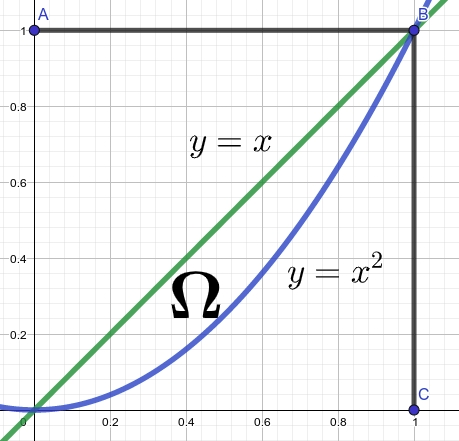
\includegraphics[width=1\textwidth]{fig7.jpg}
\end{minipage}
\begin{equation}
  \bar{f}(x,y)=
   \begin{cases}
   xy\qquad (x,y)\in \Omega\\0 \qquad altrove
   \end{cases}
\end{equation}
Chiaramente la frontiera di $\Omega$ ha misura nulla, $f$ è integrabile.
Si ha 
$$\int_0^1 \left (\int_{x^2}^x xy\ dy\right ) dx=\int_0^1 \left (\int_y^{\sqrt{y}} xy\ dx\right ) dy.$$

\section{Lezione del 26 Settembre 2018}
\subsection{Integrale iterato}
\subsubsection{Esercizio 1}
 
$\int_{\Omega}z\,dV$ \\ $\Omega$ è la regione di $\mathbb{R}^3$ limitata dal basso dal piano $xy$, lateralmente dal cilindro $x^2+y^2=1$ e da sopra dal piano $z=y$
\begin{figure}[ht]
\centering
\centerline{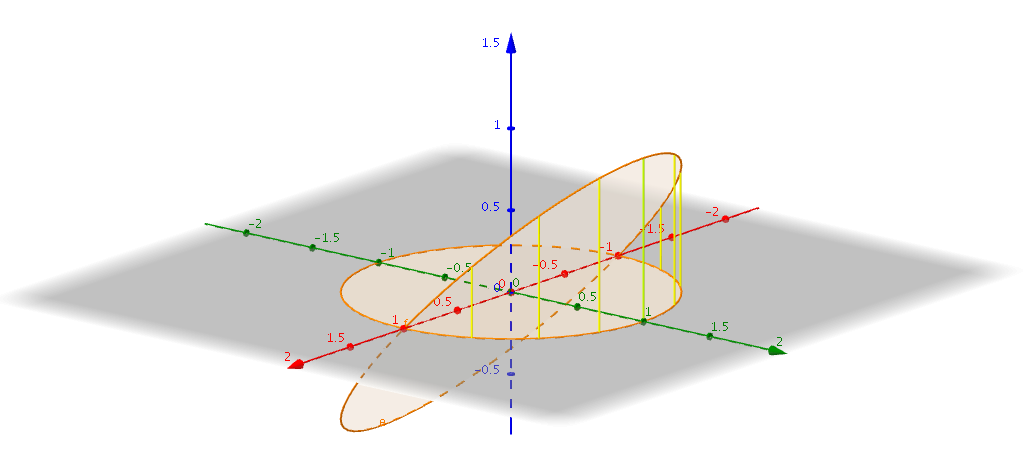
\includegraphics[width=140 mm,scale=1]{latex_img1.png}}
\label{fig: }
\end{figure}
$$\int\int\int \,dz\,dy\,dx$$ l'ultima integrazione che si fa è quella in x.
$$\Rightarrow \underbrace{\int_{-1}^{1}}_{piano xy} \underbrace{\int_{0}^{\sqrt{1-x^2}}}_{fisso x} \int_{0}^{y} z \,dz \,dy \,dx $$
$$=\frac{1}{2} \int_{-1}^{1} \int_{0}^{\sqrt{1-x^2}} y^2 \,dy \,dx = \frac{1}{6} \int_{-1}^{1} (1-x^2)^{\frac{3}{2}} \,dx =$$
Facciamo un'opportuna sostituzione \qquad $x =^s \sin{\theta} \qquad \,dx = \cos{\theta} \,d\theta$
$$= \frac{1}{6} \int_{-\frac{\pi}{2}}^{\frac{\pi}{2}} (\cos{\theta}^2)^{\frac{3}{2}} \cos{\theta} \,d\theta = \frac{1}{6} \int_{-\frac{\pi}{2}}^{\frac{\pi}{2}} |\cos{\theta}|^3 \cos{\theta} \,d\theta = \frac{1}{6} \int_{-\frac{\pi}{2}}^{\frac{\pi}{2}} (\cos{\theta})^4 \,d\theta = \frac{1}{3} \int_{0}^{\frac{\pi}{2}} (\cos{\theta})^4 \,d\theta$$
Usando la formula ricorsiva per l'integrale delle potenze del coseno:
$$\int_{0}^{\frac{\pi}{2}} cos^{2k}\theta \,d\theta = \frac{2(k-1)}{2k} \int_{0}^{\frac{\pi}{2}} cos^{2k-1}\theta \,d\theta$$
\begin{figure}[ht]
\centering
\centerline{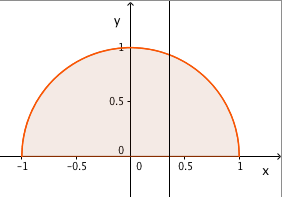
\includegraphics[width=75 mm,scale=1]{latex_img2.png}}
\label{fig: }
\end{figure}
Si può anche trovare l'integrale invertendo l'ordine delle variabili, ovviamente stando attenti agli intervalli di integrazione. Ad esempio si può iniziare considerando prima il piano yz:
$$\int \int \int z \,dx \underbrace{\,dz \,dy}$$
$$\Rightarrow \int_{0}^{1} \int_{0}^{y} \int_{-\sqrt{1-y^2}}^{\sqrt{1-y^2}}z \,dx \,dz \,dy = 2\int_{0}^{1} \int_{0}^{y} z \sqrt{1-y^2} \,dz \,dy = \int_{0}^{1} y^2 \sqrt{1-y^2} \,dy$$

\begin{figure}[ht]
\centering
\centerline{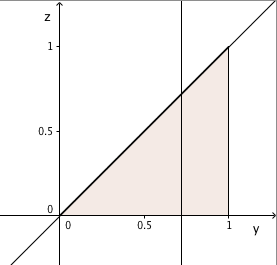
\includegraphics[width=75 mm,scale=1]{latex_img3.png}}
\label{fig: }
\end{figure}

Facciamo una sostituzione come nell'esercizio precedente \qquad $y =^s \sin{\theta}$
$$=\int_{0}^{\frac{\pi}{2}} sin^2\theta cos^2\theta \,d\theta = \int_{0}^{\frac{\pi}{2}} \left( \frac{1}{2} \sin{2\theta}\right)^2 = ...$$
Il resto dell'esercizio è lasciato al lettore.

\bigskip
Risolviamo infine lo stesso problema invertendo ancora una volta gli indici, questa volta partiamo considerando il piano xz:
$$\int \int \int z \,dy \underbrace{\,dz \,dx}$$

\begin{figure}[ht]
\centering
\centerline{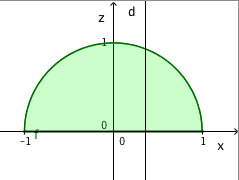
\includegraphics[width=85 mm,scale=1]{latex_img4.png}}
\label{fig: }
\end{figure}


Quando risulta difficile vedere una sezione guardando dal grafico è fondamentale trovare le relazioni analitiche che ci servono partendo dalle definizioni dell'insieme $\Omega$.
$$\begin{cases}
x^2+y^2=1 \\ z=y
\end{cases} 
\qquad \Leftrightarrow \quad x^2+z^2=1 \quad \Leftrightarrow \quad z=\pm \sqrt{1-x^2}$$
$$\Rightarrow \int_{-1}^{1} \int_{0}^{\sqrt{1-x^2}} \int_{z}^{\sqrt{1-x^2}}z \,dy \,dz \,dx = \int_{-1}^{1} \int_{0}^{\sqrt{1-x^2}} (z\sqrt{1-x^2} - z^2) \,dz \,dx =  $$
$$=\int_{-1}^{1} \left(\left[ \frac{z^2}{2} \sqrt{1-x^2} \right]_{z=0}^{z=\sqrt{1-x^2}} -\left[ \frac{z^3}{3} \right]_{z=0}^{z=\sqrt{1-x^2}}\right)\,dx = $$
$$= \int_{-1}^{1} \left( \frac{1}{2}(1-x^2)^{\frak{3}{2}} - \frac{1}{3}(1-x^2)^{\frak{3}{2}} \right)= \frac{1}{6} \int_{-1}^{1}(1-x^2)^{\frac{3}{2}} \,dx = ...$$
In tutti questi casi analizzati il risultato è lo stesso per ogni integrale, il vantaggio di invertire l'ordine delle variabili sta nel fatto che si possono semplificare molto i conti (o peggiorarli).

\subsubsection{Esercizio 2}
Supponiamo di dover calcolare il seguente integrale:
\begin{equation}
\int_0^1 \int_0^{1-x} \int_0^{x+y} f(x,y,z)\ dz dy dx.
\label{eq:int_ordine}
\end{equation}
Ci chiediamo allora quali siano gli estremi di integrazione nel caso volessimo calcolare l'integrale iterato in un ordine differente, come ad esempio prima in $y$, poi in $x$ ed infine in $z$. Possiamo provare allora a ricostruire il dominio, che chiameremo $\Omega$, della funzione a partire dagli estremi che abbiamo già.
Per come è scritta la (\ref{eq:int_ordine}), vediamo che in $\Omega$ la $x$ può assumere tutti i valori tra $0$ e $1$, la $y$ invece è vincolata ad assumere valori compresi tra $0$ e $1-x$, quindi nel piano $x$-$y$ il nostro dominio non sarà altro che il triangolo rettangolo con vertice in $(0,0)$, trovato prendendo la metà del quadrato $[0,1]\times[0,1]$. 
Per quanto riguarda l'ultima coordinata invece vediamo che la $z$ può assumere valori compresi tra $0$ e $x+y$. 
Poiché la $y$ al massimo può valere $1-x$, abbiamo che al massimo la $z$ può valere $1$, e ciò avverrà proprio sull'ipotenusa del triangolo rettangolo nel piano $x$-$y$.
Notiamo anche che per $x=0$ la $z$ vale quanto $y$, quindi nel piano $y$-$z$ il dominio sarà nuovamente un triangolo rettangolo, la cui ipotenusa però sarà data dal segmento che congiunge $(0,0)$ e $(1,1)$. 
Analogamente avverrà nel piano $x-z$, per la simmetria del dominio di $z$.
$$\Omega=\{ (x,y,z):x\in [0,1], y\in [0,1-x], z\in [0,x+y] \} .$$



\begin{minipage}{.5\textwidth}
\centering
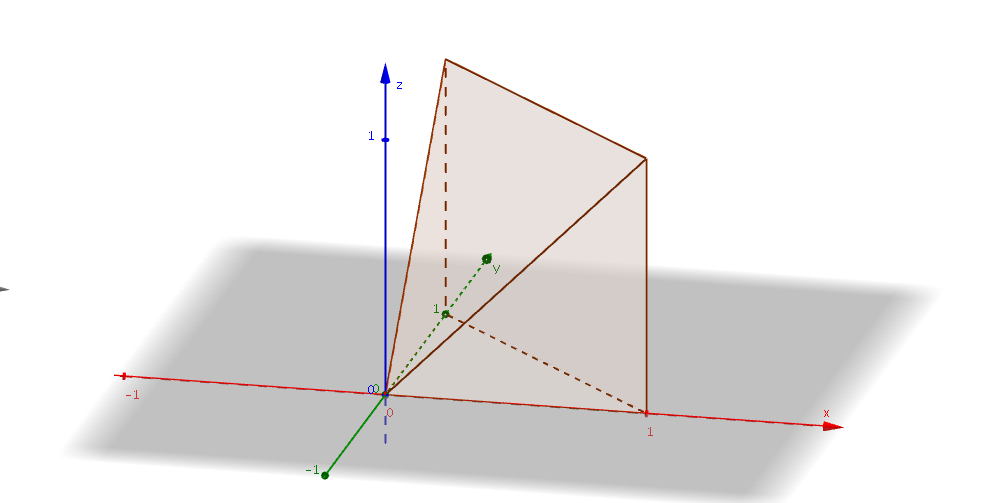
\includegraphics[width=1.5\textwidth]{fig8.png}
\end{minipage}%
\begin{minipage}{.50\textwidth}
\centering
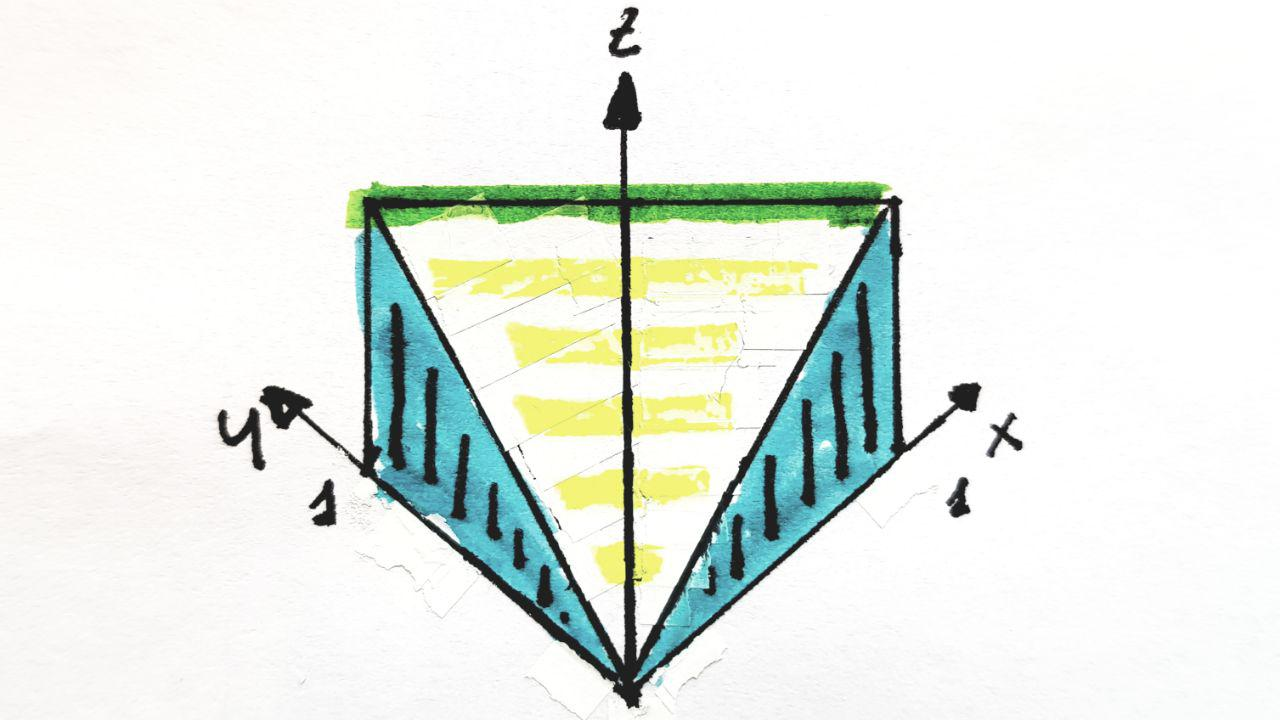
\includegraphics[width=1.4\textwidth]{fig9.jpg}
\end{minipage}
\newline
A questo punto possiamo passare a calcolarci 
$$ \int_?^?\int_?^?\int_?^?f(x,y,z)\ dy dx dz. $$
Come visto nell'esercizio precedente immaginiamo ora di proiettare tutto il dominio nel piano delle due variabili più esterne nell'integrale, nella fattispecie è quello $x$-$z$.
\newline
\begin{minipage}{.5\textwidth}
Notiamo che qui però il dominio assume una forma differente sopra e sotto il segmento che congiunge $(0,0)$ e $(1,1)$. Decidiamo allora di spezzare l'integrale in due sottodomini, consideriamo prima quello sotto il segmento. Qui la $z$ assume valori a piacere tra $0$ e $1$. La $x$ invece, una volta fissata la $z$ può assumere solamente valori compresi tra quella $z$ e $1$, infine si vede che la $y$ assume valori compresi tra $0$ e $1-x$.
\end{minipage}%
\begin{minipage}{.50\textwidth}
\centering
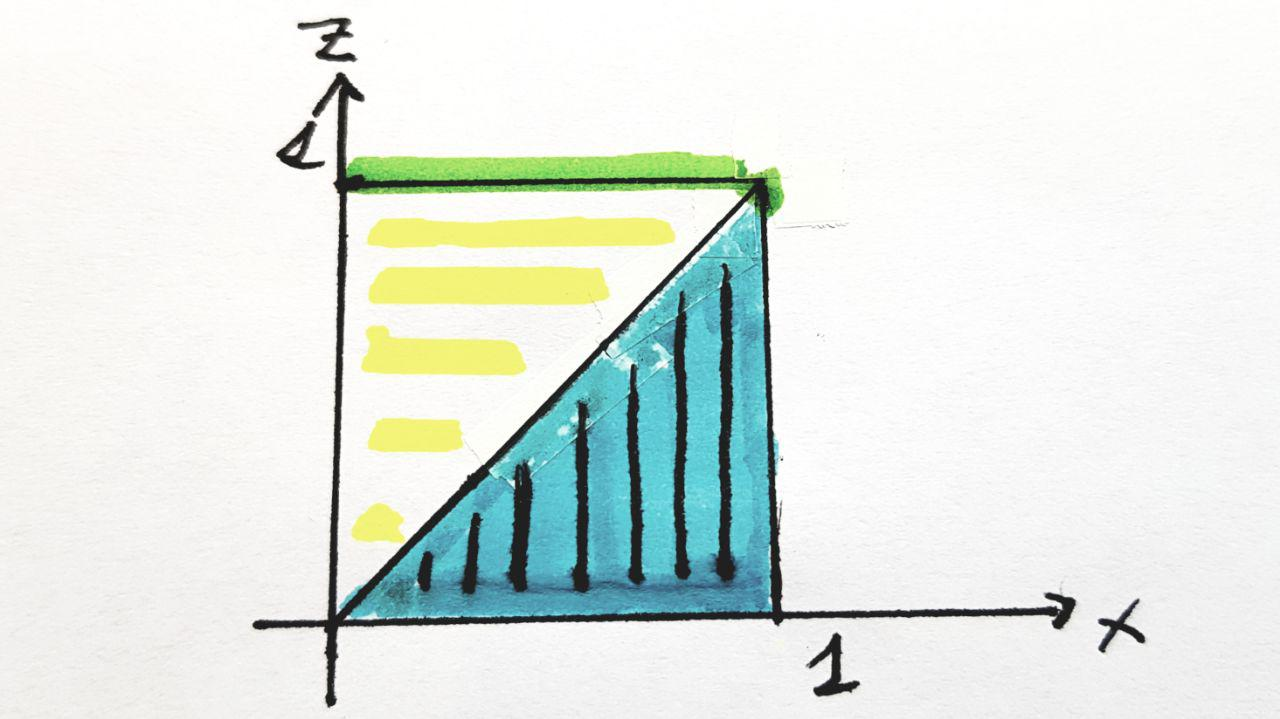
\includegraphics[width=1\textwidth]{fig10.jpg}
\end{minipage} 
Passiamo ora al sottodominio sopra il segmento. Qui la $z$ può ancora assumere valori tra $0$ e $1$, la $x$ però questa volta ha un dominio che va da $0$ a $z$ al massimo. La $y$ invece assume un intervallo di valori compreso tra $z-x$ e $1-x$. Per capire meglio quest'ultimo dominio possiamo immaginare di far passare una retta parallela alla $y$ per un punto di questo secondo sottodominio trattato, allora notiamo che entrerà all'interno  del nostro 'cuneo' $\Omega$ non per valori della $y$ pari a 0, ma nella parte gialla nel disegno, proprio dove valeva $z=x+y$.
In definitiva si ha
\begin{equation*}
\int_0^1 \int_0^{1-x} \int_0^{x+y} f(x,y,z)\ dz dy dx=
\int_0^1 \int_z^{1} \int_0^{1-x} f(x,y,z)\ dy dx dz+
\int_0^1 \int_0^{z} \int_{z-x}^{1-x} f(x,y,z)\ dy dx dz.
\label{eq:int_ordine}
\end{equation*}

\subsubsection{Esercizio 3}
Per casa. Dimostrare che
\begin{equation*}
    \int_0^x \int_0^{x_1} \int_0^{x_2}...\int_0^{x_{n-1}}f(x_n)\ dx_n dx_{n-1} ... dx_1 =
    \frac{1}{(n-1)!}\int_0^xf(t)(x-t)^n\ dt.
\end{equation*}

\subsection{Rettificabilità}
\begin{defn}
Dato $\Omega \subset \mathbb{R} ^n$ limitato, e $R$ il rettangolo in cui è iscritto, chiameremo \textit{funzione caratteristica di $\Omega$} la funzione $\chi_\Omega: R\to \mathbb{R}$ definita nel modo seguente
\begin{equation*}
  \chi_\Omega(\vec{x})=
   \begin{cases}
   1\qquad \vec{x}\in \Omega\\
   0 \qquad altrove.
   \end{cases}
\end{equation*}
\end{defn}

\begin{defn}
Dato $\Omega \subset \mathbb{R}^n$ limitato, diremo che $\Omega$ è \textit{rettificabile} se la funzione caratteristica di $\Omega$ è integrabile in $\Omega$.
Inoltre, se chiameremo volume n-dimensionale di $\Omega$
$$vol_n(\Omega) \doteq \int_\Omega \chi_\Omega \ dV = \int_R \chi_\Omega \ dV.$$
\end{defn}

\begin{thm}
$\Omega \subset \mathbb{R}^n$ limitato è rettificabile (\textit{o misurabile per Peano-Jordan}) se la frontiera di $\Omega$ ha misura nulla (\textit{volume nullo}).
\end{thm}

\section{Lezione del 28 Settembre 2018}

\subsection{Le somme di Riemann}
\begin{prop}
Sia $R \subset \mathbb{R}^n$ un rettangolo compatto (non vuoto, non degenere). Se $f:R \to \mathbb{R}^n$ è una funzione integrabile (secondo Riemann), allora $\forall \epsilon >0$, $\exists \delta >0$ tale che per ogni partizione $\mathcal{P} = \{ R_i \}$ di R per cui $diam(R_i) < \delta$ $\forall i$ valga: 
$$I^{*}(f,\mathcal{P}) - I_{*}(f,\mathcal{P}) < \epsilon$$
\end{prop}

\textit{Osservazione:}\\
Allora $\forall \epsilon >0$, $\exists \delta >0$ tale che per ogni partizione $\mathcal{P} = \{ R_i \}$ di R per cui $diam(R_i) < \delta$ $\forall i$ valga che\\
per ogni \textit{somma di Riemann} $\sum_i f(\xi_i) vol_n(R_i)$ (con $\xi_i \in R_i$),
$$\left | \int_R f\,dV - \sum_i f(\xi_i)vol_n(R_i)\right |< \epsilon$$
\\
Perché è importante?
Nelle applicazioni, in particolare in statistica, si hanno spesso somme di Riemann, anziché somme di Darboux.
\begin{defn}
Sia $T: \Omega \to \mathbb{R}$ (con $\Omega \subseteq \mathbb{R}^n$) una funzione integrabile (secondo Riemann) su $\Omega$.
Il \textit{valor medio} di T su $\Omega$ è pari a:
$$<T>_{\Omega} = \frac{\int_{\Omega} T \,dV}{vol_n(\Omega)}$$
\end{defn}

\subsection{La funzione di Thomae}

Si dice \textit{funzione di Thomae} la funzione $f:[0,1] \to \mathbb{R}$ tale che 
$$f(x) = \begin{cases} \frac{1}{q} & se\ x=\frac{p}{q} \ (ridotta\  ai\ minimi\ termini)\ con\ p,q \in \mathbb{N} \\ 1 & se\ x=0 \\ 0 & se\ x \in [0,1]\setminus \mathbb{Q} \end{cases}$$
\begin{figure}[ht]
\centering
\centerline{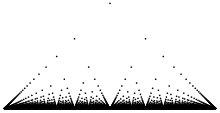
\includegraphics[width=85 mm,scale=1]{fig11.png}}
\label{fig: }
\end{figure}
\begin{lem}
Sia $f:[0,1] \to \mathbb{R}$ la funzione di Thomae, allora $\forall x_0 \in (0,1)$ vale $\lim_{x \to x_0} f(x) = 0$.
\end{lem} 
\begin{proof}
Fissiamo $\epsilon >0$ ad arbitrio.\\
Troviamo $N_{\epsilon} \in \mathbb{N}$ tale che $\frac{1}{N_{\epsilon}} < \epsilon.$\\
Allora i razionali $\frac{p}{q} \in (0,1)$ tali che $q \le N_{\epsilon}$ sono in numero finito. Fissato $x_0 \in (0,1)$, troviamo $\delta >0$ tale che $(x_0 -\delta, x_0 +\delta)$ non contiene alcun $\frac{p}{q} \in (0,1)$ (con $p,q \in \mathbb{N}$) tale che $q \le N_{\epsilon}$ (tranne al più $x_0$ stesso).\\
Scegliamo ora $x \in (0,1)$ tale che $0<|x-x_0|<\delta$.\\
Abbiamo 2 possibilità:
\begin{itemize}
    \item $x=\frac{p}{q}$ (frazione ridotta ai minimi termini) con $p,q \in \mathbb{N}$. In questo caso si ha:
    $$\left| f(x)-0 \right| = \left| f(x) \right| = \left| f\left(\frac{p}{q}\right) \right| = \frac{1}{q} < \frac{1}{N_{\epsilon}}<\epsilon$$
    \item $x \in (0,1) \setminus \mathbb{Q}$.\\
    In questo caso, si ha $f(x)=0$ e quindi:
    $$\left| f(x)-0 \right| = \left| f(x) \right| = 0<\epsilon$$
\end{itemize}
Concludiamo che $\lim_{x \to x_0} f(x) =0$ \qquad $\forall x_0 \in (0,1)$.
\end{proof}

Come conseguenza del lemma appena dimostrato, abbiamo che:
\begin{itemize}
    \item Se $x_0 \notin \mathbb{Q} \cap [0,1]$, allora\\
    $f(x_0)=0=\lim_{x \to x_0} f(x)$
    \item Se $x_0 = \frac{p}{q} \in (0,1)$ (rappresentazione minimale) con $p,q \in \mathbb{N}$, allora
    $f(x_0)=\frac{1}{q} \ne 0 = \lim_{x \to x_0} f(x)$
\end{itemize}
Dunque:
\begin{itemize}
    \item f è continua in $[0,1] \setminus \mathbb{Q}$
    \item f è discontinua in $[0,1] \cap \mathbb{Q}$
\end{itemize}
Pertanto l'insieme dei punti di discontinuità di f ha misura nulla. Inoltre f è limitata. Dunque, per il teorema di Lebesgue-Vitali, f è integrabile secondo Riemann in $[0,1]$.
\\
\textit{Osservazione:}\\ Il volume nullo dell'insieme dei punti di discontinuità è condizione non necessaria all'integrabilità.

\subsection{Tavola di Fubini}
Sia $f: R \to \mathbb{R}$ limitata con $R=[a,b]\times[c,d]\subseteq \mathbb{R}^2$ rettangolo compatto (non vuoto, non degenere). Allora vale la seguente tabella, detta \textit{Tavola di Fubini.}
{\centering
\begin{tabular}{p{0.01\textwidth}p{0.2\textwidth}|p{0.3\textwidth}|p{0.3\textwidth}}
& $$\int_R f \,dA$$ \qquad \quad esiste        & $$\int_c^d \int_a^b f(x,y)\,dx\,dy$$ \qquad \qquad \qquad esiste        &   $$\int_a^b \int_c^d f(x,y)\,dy\,dx$$ \qquad \qquad \qquad esiste      \\
\hline
& \centerline{vero}& \centerline{vero}&\centerline{vero}\\
(*)& \centerline{vero}& \centerline{falso}& \centerline{vero}\\
& \centerline{vero}& \centerline{vero}& \centerline{falso}\\
(**)& \centerline{vero}& \centerline{falso}& \centerline{falso}\\
($\sharp$)& \centerline{falso}& \centerline{vero}& \centerline{vero}\\
($\sharp\sharp$)& \centerline{falso}& \centerline{falso}& \centerline{vero}\\
& \centerline{falso}& \centerline{vero}& \centerline{falso}\\
($\dagger$)& \centerline{falso}& \centerline{falso}& \centerline{falso}\\
\end{tabular}
\par }
\bigskip
Vediamo alcuni esempi.
\\
\textbf{Caso (*)}.
$f:R\to\mathbb{R}$ con $R=[0,1]^2$ e
\begin{equation*}
  f(x,y)=
   \begin{cases}
   1\qquad x \in \mathbb{Q} \wedge y=0\\
   0 \qquad altrimenti.
   \end{cases}
\end{equation*}
Si ha allora \begin{itemize}
    \item $ \int_R f\ dA = 0 $;
    \item $ \int_0^1 f(x,y)\ dx$  non esiste per y=0;
    \item $ \int_0^1 \int_0^1 f(x,y)\ dydx = 0 = \int_R f\ dA$.
\end{itemize}
\bigskip
\bigskip

\textbf{Caso ($\dagger$)}.
$f:R\to\mathbb{R}$ con $R=[0,1]^2$ e
\begin{equation*}
  f(x,y)=
   \begin{cases}
   1\qquad (x ,y)\in \mathbb{Q} \cap [0,1]\\
   0\qquad (x ,y)\in [0,1]\setminus \mathbb{Q}.
   \end{cases}
\end{equation*}
\bigskip
\bigskip

\textbf{Caso (**)}.
$f:R\to\mathbb{R}$ con $R=[0,1]^2$ e
\begin{equation*}
  f(x,y)=
   \begin{cases}
   1\qquad (x \in \mathbb{Q} \wedge y=0)\vee (y \in \mathbb{Q} \wedge x=0)\\
   0\qquad altrimenti.
   \end{cases}
\end{equation*}
Si ha allora \begin{itemize}
    \item $ \int_R f\ dA = 0 $;
    \item $ \int_0^1 f(x,y)\ dx$  non esiste per y=0;
    \item $ \int_0^1 f(x,y)\ dy$  non esiste per x=0.
\end{itemize}
\bigskip
\bigskip

\textbf{Caso ($\sharp$)}.
$g:R\to\mathbb{R}$ con $R=[0,1]^2$ e
\begin{equation*}
  g(x,y)=
   \begin{cases}
   \frac{1}{q}\qquad x=\frac{p}{q} \wedge y=\frac{r}{q},\ con\ p,q,r \in \mathbb{N}\\
   0\qquad altrimenti.
   \end{cases}
\end{equation*}
Si ha allora \begin{itemize}
    \item $ \int_0^1 g(x,y)\ dx, \int_0^1 g(x,y)\ dy$  esistono;
    \item $ \int_R g\ dA$  non esiste.
\end{itemize}
\bigskip
\bigskip

\textbf{Caso ($\sharp \sharp$)}.
$f:R\to\mathbb{R}$ con $R=[0,1]^2$ e
\begin{equation*}
  f(x,y)=
   \begin{cases}
   1\qquad x \in \mathbb{Q} \wedge y=0\\
   0\qquad x \notin \mathbb{Q} \wedge y=0\\
   g(x,y)\qquad altrimenti.
   \end{cases}
\end{equation*}
Dove per $g(x,y)$ prendiamo quella definita nel caso ($\sharp$).
Si ha allora 
\begin{itemize}
    \item $ \int_R f\ dA$ non esiste;
    \item $ \int_0^1 f(x,y)\ dx$  non esiste per y=0;
    \item $ \int_0^1 f(x,y)\ dy$  esiste.
\end{itemize}

\bigskip
Nel resto della lezione è stato dimostrato il teorema \textit{Baby Fubini} (\ref{th: baby_fubini}), la dimostrazione si può trovare direttamente nella sottosezione (\ref{sec: babyfub}).


\section{Lezione del 03 Ottobre 2018}

\subsection{Insiemi \textit{normali}}
\begin{defn}
Sia $K\subset \mathbb{R}^{n-1}$ compatto rettificabile. $\alpha , \beta:K\to \mathbb{R}$ siano continue e tali che $\alpha(\vec{x})\leq \beta(\vec{x}),\ \forall \vec{x} \in K$. Diremo allora \textit{normale} (rispetto a $\mathbb{R}^{n-1}$) il sottoinsieme $N$ di $\mathbb{R}^n$ definito come
$$N\doteq \{ (\vec{x},t)\in \mathbb{R}^n: \vec{x} \in K, \alpha(\vec{x})\leq t \leq \beta(\vec{x}) \}. $$
\end{defn}

\begin{thm}
Ogni insieme normale $N$ in $\mathbb{R}^n$ è un compatto rettificabile. Vale
$$vol_n(N) = \int_N dV_n = \int_K (\beta(\vec{x}-\alpha(\vec{x})\ dV_{n-1}.$$
\end{thm}

Ecco un corollario di questo teorema.
\begin{cor}
Siano $N_1,...,N_L$ insiemi normali in $\mathbb{R}^n$ (non necessariamente rispetto allo stesso insieme di $\mathbb{R}^{n-1}$) disgiunti a coppie, allora si ha che $N$, definito come
$$N=\bigcup_{k=1}^L N_k, $$ è compatto e rettificabile.
\end{cor}

\begin{thm}
Sia $N$ insieme normale in $\mathbb{R}^n$ e sia $f:N\to \mathbb{R}$ continua. Allora vale 
$$\int_N f\ dV_n = \int_K \int_{\alpha(\vec{x})}^{\beta(\vec{x})} f(\vec{x}, t)\ dt\ dV_{n-1} .$$
\end{thm}
Vediamo ora qualche esempio di utilizzo di questi teoremi nel calcolo di aree e volumi.
\subsubsection{Esercizio 1}
Sia l'insieme $C\subset \mathbb{R}^2$ limitato dal semicerchio di centro $(0,1)$, raggio $1$ e contenuto nel primo quadrante. La circonferenza intera da cui poi prendiamo metà area avrebbe equazione $x^2+(y-1)^2=1$.
Vogliamo calcolare l'area della funzione $f(x,y)\doteq xy$ definita in $C$, ovvero 
$\int_C xy\ dA$. Posso vedere $C$ come insieme normale rispetto all'asse delle $y$.
Allora lo scrivo nel seguente modo
$$C=\{ (x,y)\in \mathbb{R}^2:y\in [0,2],\ x \in [0,\sqrt{1-(y-1)^2}] \}.$$
Avendo definito così l'insieme allora 
$$\int_C xy\ dA = \int_0^2 \int_{\alpha(y)}^{\beta(y)} xy\ dx\ dy=\int_0^2 \int_0^{\sqrt{2y-y^2}} xy\ dx\ dy = \int_0^2 \frac{(2y-y^2)}{2}y\ dy = \frac{2}{3}.$$
Chiaramente era una possibilità anche quella di vedere $C$ come normale rispetto all'asse delle ascisse. In questo caso
$$C=\{ (x,y)\in \mathbb{R}^2:x\in [0,1],\ y \in [1-\sqrt{1-x^2},1+\sqrt{1-x^2}] \},$$
poiché da $x^2+(y-1)^2=1$ si ottiene $y=1 \pm \sqrt{1-x^2}$.
Allora l'integrale diventa 
$$\int_C xy\ dA = \int_0^1 \int_{1-\sqrt{1-x^2}}^{1+\sqrt{1-x^2}} xy\ dy\ dx=\frac{1}{2} \int_0^1  x[y^2]_{1-\sqrt{1-x^2}}^{1+\sqrt{1-x^2}}\ dx = 2 \int_0^1  x\sqrt{1-x^2}\ dx =...=\frac{2}{3}.$$
Come ci aspettavamo il risultato è lo stesso, vediamo ora un caso tridimensionale.

\subsubsection{Esercizio 2}
Sia $E\subset \mathbb{R}^3$ definito come
$$E=\{ (x,y,z)\in \mathbb{R}^3:x\geq 0,\ z\geq 0,\  0\leq y\leq 2-x^2-z^2 \}.$$
Come si può vedere in figura il $E$ è la parte di un paraboloide che sta nel primo ottante. Vogliamo calcolare $\int_E xz\ dV_3$, vediamo il nostro insieme come normale rispetto ad un insieme $K\subset \mathbb{R}^2$ che sta nel piano $x$-$y$:
$$K=\{ (x,y)\in \mathbb{R}^2:x \in [0,\sqrt{2}],\ y\in [0,2-x^2] \}.$$
In questo caso le due funzioni che delimitano $z$ sono $\alpha (x,y)=0$ dal basso e $\beta (x,y)=\sqrt{2-x^2-y}$ da sopra.
Allora 
$$\int_E xz\ dV_3=\int_K \int_0^{\sqrt{2-x^2-y}} xz\ dz\ dA=\int_0^{\sqrt{2}} \int_0^{2-x^2} \int_0^{\sqrt{2-x^2-y}} xz\ dz\ dy\ dx$$
$$ = \frac{1}{2}\int_0^{\sqrt{2}} \int_0^{2-x^2} (2-x^2-y)\ dy\ dx = ... = \frac{1}{3}.$$

\subsection{\textit{Supporto} di una funzione}

\begin{defn}
$A\subset \mathbb{R}^n$ aperto, $f:A\to \mathbb{R}$. Diremo \textit{supporto di $f$} l'insieme
$$supp (f)\doteq cl_A ( \{ \vec{x} \in A: f(\vec{x})\neq 0 \}) .$$
\end{defn}

A titolo di esempio possiamo trovare il supporto della funzione caratteristica di $A$, che chiameremo $\chi_A$. 
Allora poiché per definizione la funzione assume valori nulli fuori da $A$
$$supp( \chi_A) = cl_A (\{ \vec{x} \in A: \chi_A(\vec{x})\neq 0 \}) = A.$$

\begin{lem}
$f:\mathbb{R}^n\to \mathbb{R}$. L'insieme $supp(f)$ è sempre un chiuso, inoltre se è anche limitato allora si tratta di un compatto.
\end{lem}
La dimostrazione è una banale applicazione del teorema di Heine-Borel.
\\
\\ Se $f$ ha supporto compatto ed è differenziabile con continuità $k$ volte in $\mathbb{R}^n$ scriveremo che $f\in \mathcal{C}_0^k (\mathbb{R}^n).$
\\
\textit{Osservazione:}
\\
$f:\mathbb{R}^n\to \mathbb{R}$. Se $f$ è continua e ha supporto compatto ($f\in \mathcal{C}_0^0 (\mathbb{R}^n)$) allora ha senso
$$\int_{\mathbb{R}^n} f\ dV_n = \int_{supp(f)} f\ dV_n. $$


\subsubsection{Esempio 1}
Sia data la funzione $f(x):\mathbb{R} \to \mathbb{R}$ definita:

$$f(x):
\begin{cases}
 \neq 0 & x \in (1,3) \cup (3,4) \cup (4,5) \\
 =0 & altrimenti
\end{cases}$$
Trovo la chiusura in $\mathbb{R}$ dell'insieme dei punti in cui la funzione assume valori diversi da $0$, quindi 
$$supp (f) = \overline{(1,3) \cup (3,4) \cup (4,5)} = [1,5] $$

%\begin{figure}[ht]
%\centering
%\centerline{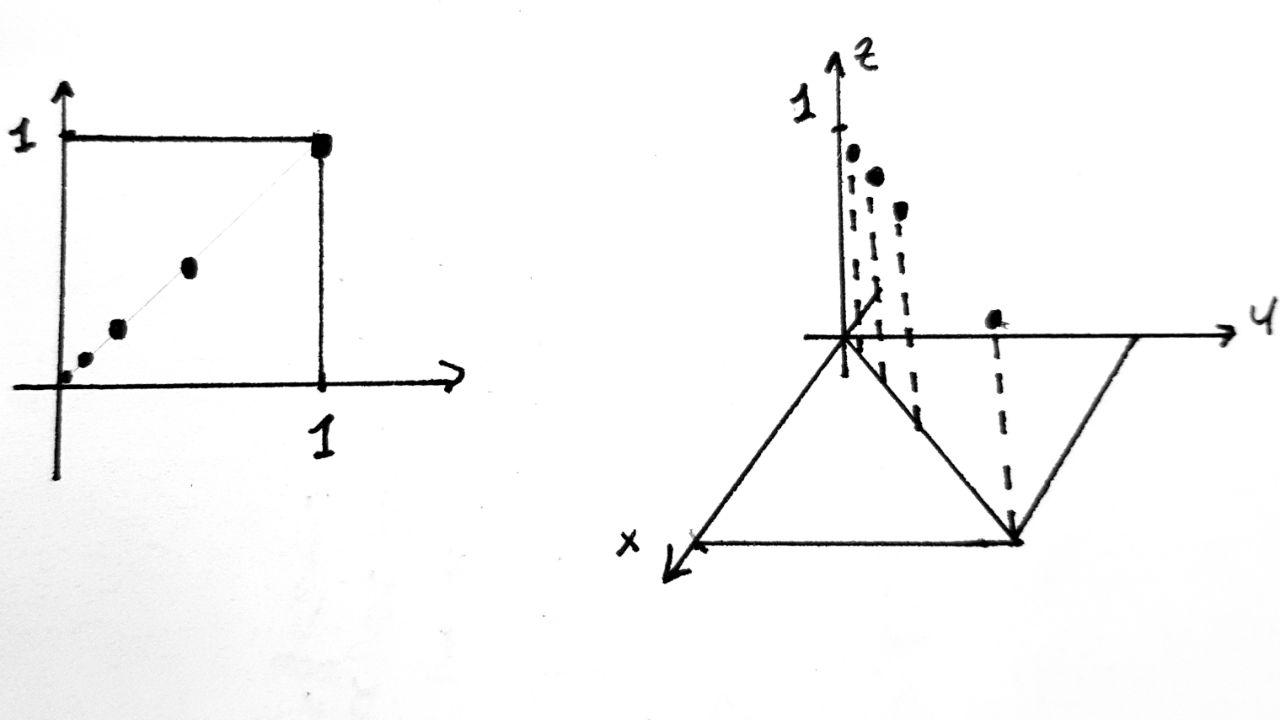
\includegraphics[width=93 mm,scale=1]{fig6.jpg}}
%\label{fig: }
%\end{figure}

\subsubsection{Esempio 2}
Sia data la funzione $f: B(\vec{0},1) \subseteq \mathbb{R}^2 \to \mathbb{R}$ definita:
$$f(x,y)=
\begin{cases}
 0 & x \leq 0 \\
 x & x > 0
\end{cases}$$
L'insieme che ci interessa analizzare è $\{ (x,y) \in B(\vec{0},1): f(x,y) \neq 0 \}$, quindi il supporto di f sarà dato dalla chiusura (rispetto alla palla aperta B) di questo insieme. Si ha
$$supp(f) = cl_{B(\vec{0},1)} (\{ (x,y) \in B(\vec{0},1): f(x,y) \neq 0 \}) = \{(x,y) \in B(\vec{0},1) \; | \; x\geq 0 \}$$
In questo esempio $f$ non è una funzione a supporto compatto, perché il supporto non è limitato, infatti la frontiera di B è infinita rispetto a B.\\
%\begin{figure}[ht]
%\centering
%\centerline{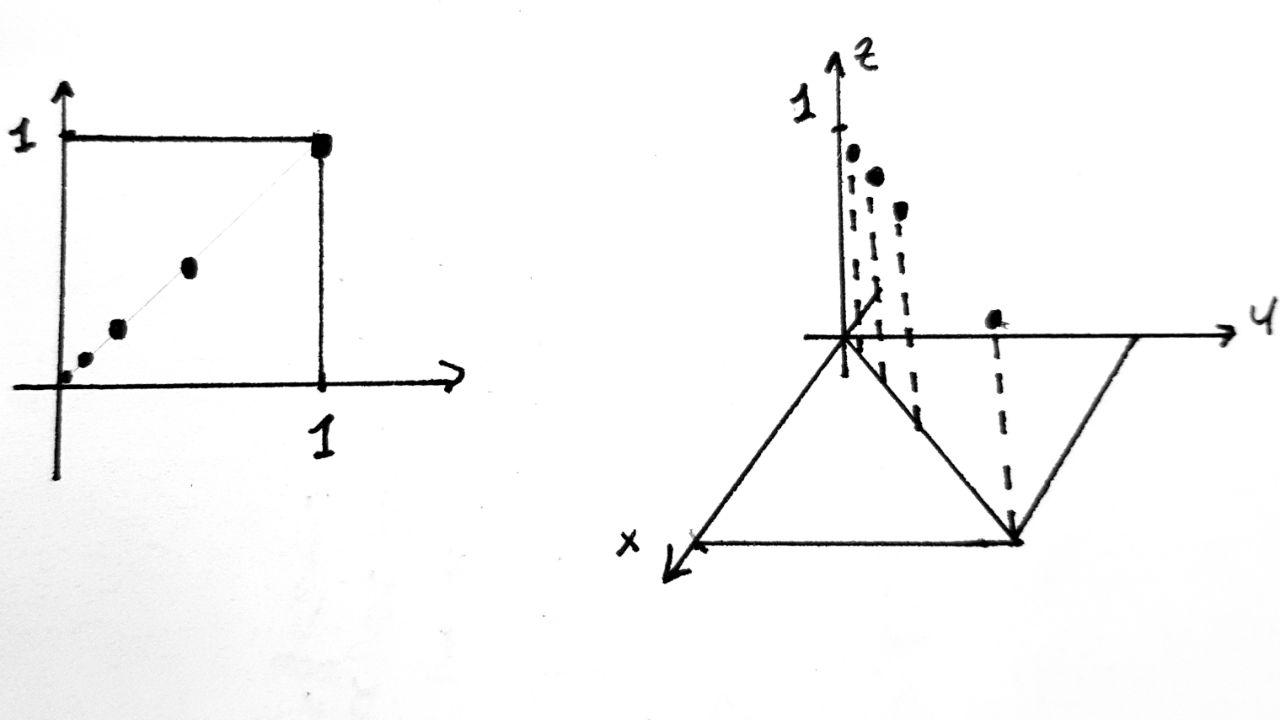
\includegraphics[width=93 mm,scale=1]{fig6.jpg}}
%\label{fig: }
%\end{figure}
\textbf{NB}: Quando si studiano le aperture e chiusure degli insiemi bisogna sempre pensare rispetto alla topologia di quale altro insieme queste sono riferite. Nell'esempio sopra la palla $B$ risulta non limitata se la sua limitatezza è studiata a partire da $B$ stesso, mentre l'insieme $B$ risulta limitato se riferito ad esempio a $\mathbb{R}^2$. 

\subsubsection{Esempio 3}
Prendendo come insieme di definizione l'esempio di prima, $\{ (x,y) \in B(\vec{0},1): f(x,y) \neq 0 \}$, definiamo $f$ come
$$f(x,y)=
\begin{cases}
 -x(x^2 + y^2 -1) & \sqrt{x^2 + y^2} \leq 1 \\
 0 & altrimenti
\end{cases}$$
Il supporto in questo caso è dato dalla chiusura di $B$ stesso: $supp(f) = \overline{B(\vec{0},1)}$
\\
\subsubsection{Esempio 4}
Prendendo anche in questo caso insieme di definizione dell'esempio precedente, $\{ (x,y) \in B(\vec{0},1): f(x,y) \neq 0 \}$, definiamo $f:B(\vec{0},1)\to \mathbb{R}$ come
$$f(x,y)=
\begin{cases}
 0 & \sqrt{x^2 + y^2} > \frac{1}{2} \\
 \frac{1}{2}-\sqrt{x^2 + y^2} & \sqrt{x^2 + y^2} \leq \frac{1}{2}
\end{cases}$$
Il supporto è dato da $supp(f) = cl(\{ (x,y) \in B(\vec{0},1) : f(x,y) \neq 0\})= \overline{B(\vec{0},1)}$, quindi ciò equivale al disco $C=D[\vec{0},\frac{1}{2}]$, infatti se interseco $C$ con $B$ ottengo la sempre la chiusura di $B$.


\section{Lezione del 05 Ottobre 2018}

\subsection{Integrazione in coordinate polari}

Talvolta quando l'integrazione su domini particolari si fa troppo complicata è utile passare a coordinate polari per semplificare l'integrazione. Vediamo di seguito alcuni esempi di trasformazione di domini da coordinate cartesiane a polari. Queste ultime in $\mathbb{R}^2$ determinano la posizione di un punto $P$ attraverso la distanza dall'origine $\rho$ del punto e dall'angolo che la congiungente di $P$ e $O$ forma con uno degli assi. Di seguito chiameremo $\theta$ l'angolo formato con l'asse delle ascisse e preso positivo in senso antiorario. Chiaramente allora si avrà
\begin{equation}
\begin{cases}
x=\rho \cos{\theta}\\
y=\rho \sin{\theta}
\end{cases}     
\label{eq: polari}
\end{equation}
 
\subsubsection{Esempio 1}

Supponiamo di avere una circonferenza centrata in $\vec{O} \in \mathbb{R}^2$ e con raggio $a$. Chiaramente allora essendo $a=\rho$ costante per tutti i valori di $\theta$, nel grafico $\rho$-$\theta$ la circonferenza sarà rappresentata da un semplice segmento verticale.

\subsubsection{Esempio 2}

Supponiamo invece ora di avere una verticale in coordinate cartesiane, di equazione $y=a$. Possiamo trovare l'equazione che descrive la curva in coordinate polari semplicemente mettendo a sistema quella in coordinate cartesiane e $y=\rho \sin{\theta}$, ottenendo così $\rho=\frac{1}{\cos{\theta}}$, con $\theta \in (-\frac{\pi}{2}; \frac{\pi}{2})$. 

\subsubsection{Esempio 3}

Vogliamo trovare il corrispondente in coordinate polari di una circonferenza di raggio reale $a$ centrata in $(a,0)$. Il metodo più veloce per farlo è notare che preso un qualsiasi punto $P$ sulla circonferenza vale la relazione 
$$\cos{\theta}=\frac{\rho}{2a} \Leftrightarrow \rho = 2a\cos{\theta}.$$
Un metodo più tradizionale e applicabile alla maggior parte dei casi è invece quello di prendere l'equazione della curva ($(x-a)^2+y^2=a^2$ in questo caso) e dopo averla messa a sistema con la ($\ref{eq: polari}$) trovare i valori di $\rho$ (o $\theta$).

\subsubsection{Esempio 4}
Non sono rari i casi di figure \textit{esotiche} con complesse equazioni se scritte in coordinate cartesiane che si semplificano non di poco con la trasformazione alle polari. 
\begin{itemize}
    \item \textbf{Esempio 4.a}
    \\ Il \textit{cardioide}, in coordinate cartesiane 
    $$(x^{2}+y^{2})^{2}+4ax(x^{2}+y^{2})-4a^{2}y^{2}=0, $$
    se espresso in polari diventa 
    $$\rho= a(1+\cos{\theta})$$.
    
    \item \textbf{Esempio 4.b}
    \\ La \textit{spirale archimedea} in polari è semplicemente $\rho = a+b\theta$. Può altrimenti essere espressa in coordinate parametriche come $$ \begin{cases}x(\theta )=(a+b\theta )\cos \theta \\y(\theta )=(a+b\theta )\sin \theta \end{cases}$$

    \item \textbf{Esempio 4.c}
    \\ La \textit{lemniscàta di Bernoulli} è una curva algebrica a forma di otto coricato: essa ha un biflecnodo nell'origine, e due punti doppi nodali nei punti cilici; è descritta in coordinate cartesiane nella forma:
    $$    (x^{2}+y^{2})^{2}=2a^{2}(x^{2}-y^{2})$$ e in coordinate polari si può scrivere come $ \rho^{2}=2a^{2}\cos 2\theta$.
    
\end{itemize}
\bigskip
\begin{thm}
Chiamata $\vec{g}(\rho, \theta) = (x,y) = (\rho \cos \theta, \rho \sin \theta)$ la funzione che trasforma coordinate polari in cartesiane, dato $\Omega$ compatto, e chiamata $S$ la controimmagine di $\Omega$ ($\vec{g} (S)=\Omega $), vale
$$\int_{\Omega} f(x,y)\ dA_{xy} = \int_S (f\circ \vec{g}) (\rho, \theta) \rho \ d\rho d\theta. $$
\end{thm}

La dimostrazione a livello intuitivo consiste nel fatto che se prendiamo un rettangolo infinitesimo qualsiasi, che chiameremo $S$, in coordinate polari la sua area sarà data da $dA=d\rho d\theta$. Se prendiamo ora invece l'area corrispondente in coordinate cartesiane, che chiameremo $\Omega = \vec{g} (S)$, notiamo che $\Omega$ non è altro che una frazione infinitesima di area di un settore circolare di angolo $d\theta$ di una circonferenza di raggio $\rho$. Chiaramente possiamo allora scrivere quell'area come l'arco che racchiude il settore circolare ($\rho d\theta$) per l'incremento infinitesimo del raggio $d\rho$. 


\bigskip

\textbf{Problema}\\
\textbf{0.}
\newline
Come esempio di applicazione delle coordinate polari a problemi meno banali possiamo chiederci quale sia la distanza media di un punto qualsiasi di un quadrato da un suo vertice.
\\ Chiamiamo $Q=[0,1]\times [0,1]$ il quadrato in analisi, vogliamo allora calcolare 
$$\langle dist(\vec{O}, \vec{P} \rangle _Q = \frac{1}{area(Q)}\int_Q \sqrt{x^2+y^2}\ dA, $$ dove $\vec{P}$ è un punto qualsiasi appartenente a $Q$.
\\ Vale sempre 
\begin{equation*}
\vec{g}=
\begin{bmatrix}
\rho \cos{\theta}\\
\rho \sin{\theta}
\end{bmatrix}   
=
\begin{bmatrix}
x\\
y
\end{bmatrix}   
\end{equation*}
quindi
$$D\vec{g}=
\begin{bmatrix} 
\vec{\Delta}g_1 \\
\vec{\Delta}g_2
\end{bmatrix}
= [ \partial_{\rho}\vec{g} , \quad \partial_{\theta}\vec{g}] = \begin{bmatrix} 
\cos{\theta} & -\rho\sin{\theta} \\
\sin{\theta} & \rho\cos{\theta}
\end{bmatrix} 
\Rightarrow det (D\vec{g})=\rho.$$ 
E sappiamo che vale che l'area del parallelogramma formato da due vettori $\vec{v}_1$ e $\vec{v}_2$ è $Area = det[\vec{v}_1 , \vec{v}_2]$.
Di conseguenza
$$\int_{Q=\Omega} \sqrt{x^2+y^2} \,dA_{xy} = \int_S \rho^2 \,d\rho \,d\theta$$ \\
Sfruttando la simmetria del problema, trasformo solo il triangolo in coordinate polari, quindi posso riscrivere
$$2\int_{\triangle} \sqrt{x^2+y^2} \,dA_{xy} = 2\int_{S/2} \rho^2 \,d\rho \,d\theta = 2\int_0^{\frac{\pi}{4}} \,d\theta \int_0^{\sec \theta} \rho^2 \,d\rho = \frac{2}{3} \int_0^{\frac{\pi}{4}} \sec^3 \theta \,d\theta = (*).$$
Vale la formula
$$\int \sec^k \theta \,d \theta = \int \sec^{k-2}\theta \sec^2 \theta \,d\theta = \int \sec^{k-2} \theta (1+\tan^2 \theta) \,d \theta,$$
quindi
$$(*)= \frac{2}{3} \left( \frac{1}{4} \log|\sec\theta+\tan\theta|+\frac{1}{2} \tan\theta\sec\theta \right)_{\theta=0}^{\theta=\frac{\pi}{4}} = \underbrace{\frac{1}{3} (\log(1+\sqrt{2})+\sqrt{2}) = 0.59899}_{Distanza\ media\ dai\ punti\ dell'origine}.$$
%\begin{figure}[ht]
%\centering
%\centerline{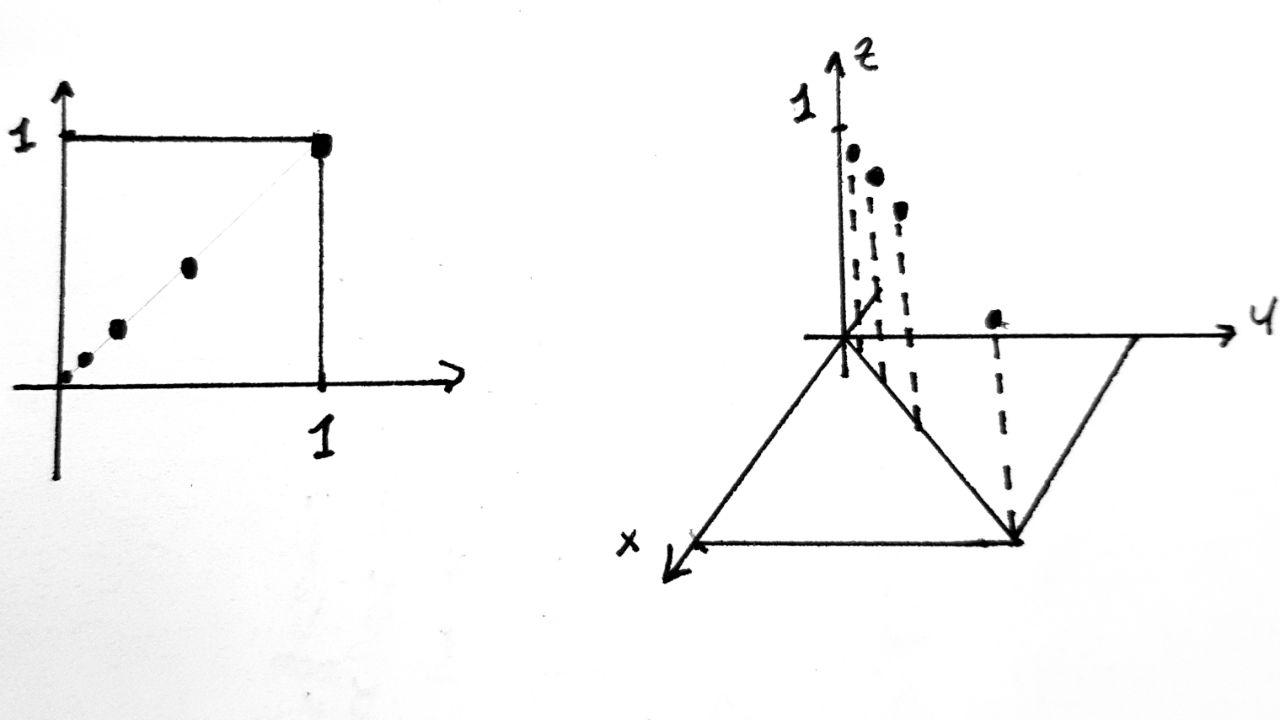
\includegraphics[width=93 mm,scale=1]{fig6.jpg}}
%\label{fig: }
%\end{figure}
\bigskip
\textbf{1.}
$$\int_0^1 \,dx \int_0^1 \frac{ye^y}{x^2+y^2} \,dy =\int_{\Omega} f \,dA $$
Passando da coordinate cartesiane a polari
$$\int_S \frac{\rho \sin\theta e^{\rho\sin\theta}}{\rho^2}\rho \,d\rho \,d\theta $$
$$= \int_{\frac{\pi}{4}}^{\frac{\pi}{2}}\,d\theta \int_0^{\csc\theta} \sin\theta e^{\rho\sin\theta}\,d\rho = \int_{\frac{\pi}{4}}^{\frac{\pi}{2}} \,d\theta \int_0^{\csc\theta} d(e^{\rho\sin\theta}) = \int_{\frac{\pi}{4}}^{\frac{\pi}{2}} \underbrace{\left[ e^{\rho\sin\theta}\rceil_{\rho=0}^{\rho=\csc\theta}\right]}_{e-1} \,d\theta = \frac{\pi}{4}(e-1).$$
\textbf{2.}\newline
$\Omega$ regione limitata da sopra da $x^2+y^2=4y$ e da sotto da $y=2$. Sia $$f(x,y) = \frac{y^2}{(x^2+y^2)^{1/2}}.$$
Si trova facilmente che
$$\int_{\Omega}f \,dA = \dots = \frac{1}{3\sqrt{2}}.$$
\bigskip
\textbf{3.}\newline
Le coordinate polari sono un grande aiuto per integrare anche la funzione degli errori di Gauss (integrale di Eulero-Poisson).
$$I = \int_0^{\infty} e^{-x^2} \,dx = ? = \frac{\sqrt{\pi}}{2}$$
$$I^2 = \left( \int_0^{\infty} e^{-x^2} \,dx \right)^2 = \int_0^{\infty} e^{-x^2} \,dx \int_0^{\infty} e^{-y^2} \,dy = \int_0^{\infty} \int_0^{\infty} e^{-x^2} e^{-y^2} \,dx \,dy $$ $$= \int_0^{\infty} \int_0^{\infty} e^{-(x^2+y^2)} \,dx \,dy = \int_0^{\frac{\pi}{2}} \int_0^{\infty} e^{-\rho^2} \rho \,d\rho = \frac{\pi}{4} e^{-\rho^2} \rceil_{\rho=0}^{\rho=\infty} = \frac{\pi}{4} $$ $$ \Rightarrow I=\frac{\sqrt{\pi}}{2}$$.

\section{Lezione del 10 Ottobre 2018}

\subsection{Integrazione in coordinate cilindriche}

Le coordinate cilindriche in $\mathbb{R}^3$ sono descritte dalla terna ($r,\theta,z$). $r$ rappresenta il raggio della base del cilindro, $\theta$ l'angolo descritto dal raggio (analogamente alle coordinate polari in $\mathbb{R}^2$), infine $z$ corrisponde all'omonima coordinata nel sistema di riferimento cartesiano.\\
Passaggio di coordinate da cilindriche a cartesiane
$$\vec{g} \left(\begin{matrix}  r \\ \theta \\ z  \end{matrix}\right) = \begin{bmatrix} x \\ y \\ z \end{bmatrix} = \begin{bmatrix} r \cos\theta \\ r \sin\theta \\ z \end{bmatrix}$$
Il volume infinitesimo nelle coordinate cartesiane è $\,dV = \,dx\,dy\,dz$ , mentre nelle coordinate cilindriche $\,dV = r\,dz\,dr\,d\theta$, per motivi analoghi a quelli esposti nella sezione sulle coordinate polari in $\mathbb{R}^2$.
%\begin{figure}[ht]
%\centering
%\centerline{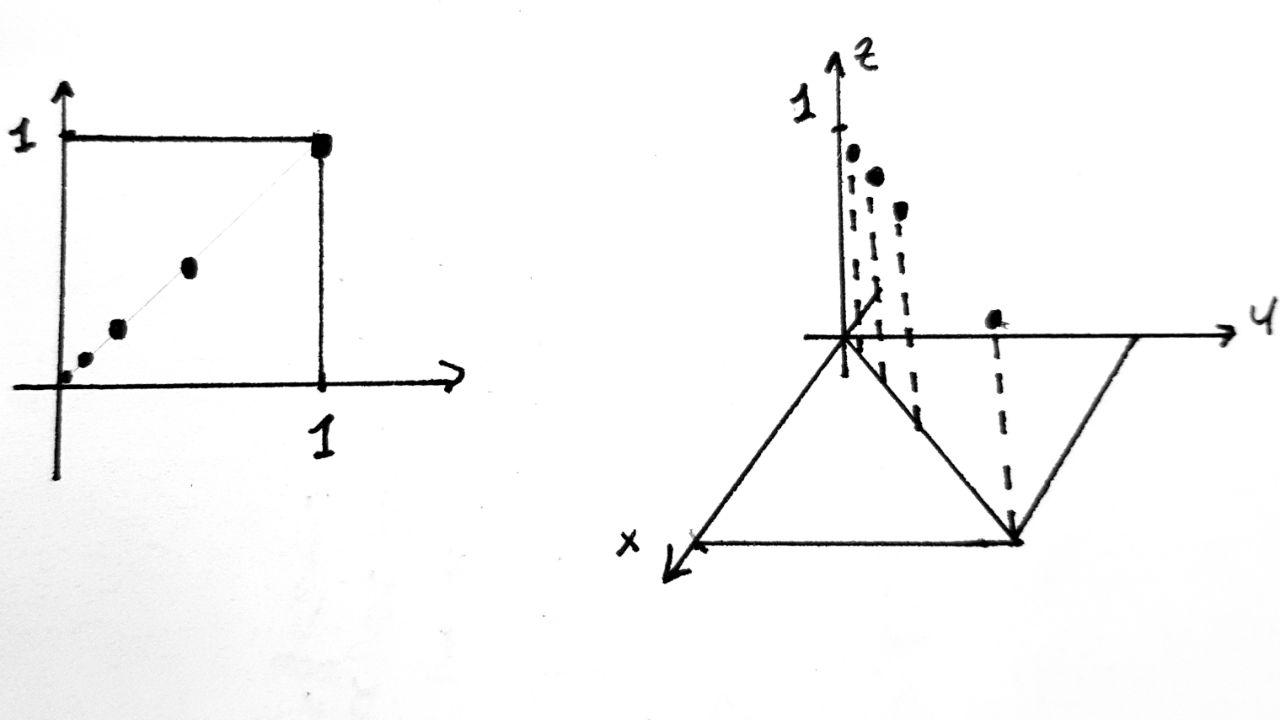
\includegraphics[width=93 mm,scale=1]{fig6.jpg}}
%\label{fig: }
%\end{figure}

\subsubsection{Esercizio 1.}
Calcolare il volume di un cilindro di raggio $a$ e altezza $h$.
$$Vol_3(C)=\int_C 1\,dV =\int_0^{2\pi}\int_0^a \int_0^h r\,dz\,dr\,d\theta = 2\pi \cdot h \cdot \frac{a^2}{2} = \pi a^2 h$$
l'integrale è stato fatto sfruttando le simmetrie del problema (cilindro), facendo uso delle coordinate cilindriche. Sopra il volume è stato integrato \textit{per filo}, ma un analogo risultato si poteva ottenere facendo un'integrazione \textit{per strati}.
$$Vol_3(C)=\int_0^h A_s(z)\,dz,$$ con $A_s$ area della sezione.

\subsubsection{Esercizio 2.}
Sia $\Omega$ limitata da sopra dalla sfera $x^2+y^2+z^2 = 6$ e dal basso dal paraboloide $z=x^2+y^2$. Calcolare allora $\int_{\Omega} z\,dV$.\\
$\Omega$ risulta essere simmetrico per rotazioni attorno all'asse $z$, quindi possiamo ricondurci alle coordinate cilindriche, facendo le opportune sostituzioni. Vale
$$\int_{\Omega} z\,dV = \int_0^{2\pi}\int_0^{\sqrt{2}}\int_{r^2}^{\sqrt{6-r^2}} z\,r\,dz\,dr\,d\theta = \ldots = \frac{11}{3} \pi.$$
L'intervallo di integrazione della variabile $\theta$ va da $[0,2\pi]$ per la simmetria lungo l'asse $z$. Per trovare Quello relativo alla variabile $r$, faccio la proiezione di $\Omega$ sul piano $z=0$ oppure trovo l'intersezione tra la paraboloide e la sfera. Quindi prima cambio coordinate poi faccio l'intersezione delle due curve:
$$\begin{cases}
 z=x^2+y^2 \\ x^2+y^2+z^2 =6
\end{cases} \Rightarrow 
\begin{cases}
 z=r^2 \\ r^2+z^2 =6
\end{cases} $$
$$\Rightarrow z^2+z-6=0 \Rightarrow (z-2)(z+3)=0 \Rightarrow z=2 \ \vee \ \text{\sout{$z=-3$}} \Rightarrow r=\sqrt{2}$$
Infine per l'intervallo di integrazione della variabile $z$ considero una retta verticale parallela all'asse $z$, e vedo che questa retta entra in $\Omega$ attraverso il paraboloide ($z=r^2$) ed esce dalla sfera ($z=\sqrt{6-r^2}$).
%\begin{figure}[ht]
%\centering
%\centerline{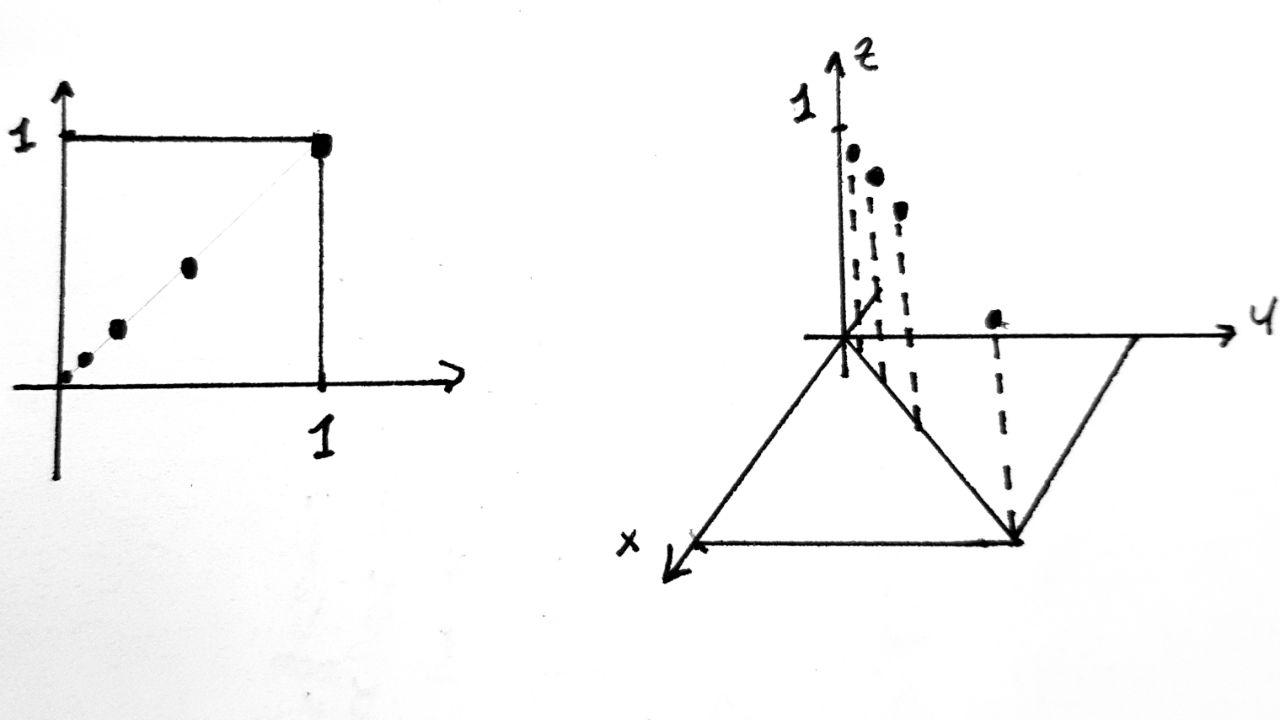
\includegraphics[width=93 mm,scale=1]{fig6.jpg}}
%\label{fig: }
%\end{figure}

\subsubsection{Esercizio 3.}
Qual è la distanza quadratica media dei punti del cilindro rispetto all'asse di simmetria?\\
Integro sul volume del cilindro la distanza di ogni punto dall'asse di simmetria ($z$).
$$\int_{\Omega} dist(\vec{x},A)^2 \,dV$$
La distanza di un punto dall'asse si può scrivere in coordinate cartesiane come $dist(\vec{x},A) = \sqrt{x^2+y^2}$ a $z$ costante. Quindi passando in coordinate cilindriche
$$=\int_{\Omega} (x^2+y^2)\,dV = \int_0^{2\pi} \int_0^a\int_0^h \underbrace{r^2 \cdot r}_{r^3} \,dz\,dr\,d\theta = 2\pi h \frac{a^4}{4} = (\pi a^2 h)\cdot\frac{a^2}{2}$$
Questo non è altro che il procedimento per il calcolo del \textbf{momento di inerzia}.
\subsubsection{Esercizio 4.}
$\Omega$ limitata dal paraboloide $z=6-x^2-y^2$ e dal cono $z=\sqrt{x^2+y^2}$
$$\int_{\Omega} z\,dV = \int_0^{2\pi}\int_0^{2}\int_{r}^{6-r^2} z\,r\,dz\,dr\,d\theta = \ldots = \frac{92}{3} \pi$$
Seguendo la stessa procedura dell'esercizio 2, si trova l'intervallo di integrazione per la variabile $r$
$$\begin{cases}
 z=6-x^2-y^2 \\ z=\sqrt{x^2+y^2}
\end{cases} \Rightarrow 
\begin{cases}
 z=6-r^2 \\ z=r
\end{cases}\Rightarrow r=2$$
Mentre per la variabile $z$ sappiamo che entriamo dal cono ($z=r$) ed usciamo dal paraboloide ($z=6-r^2$).
%\begin{figure}[ht]
%\centering
%\centerline{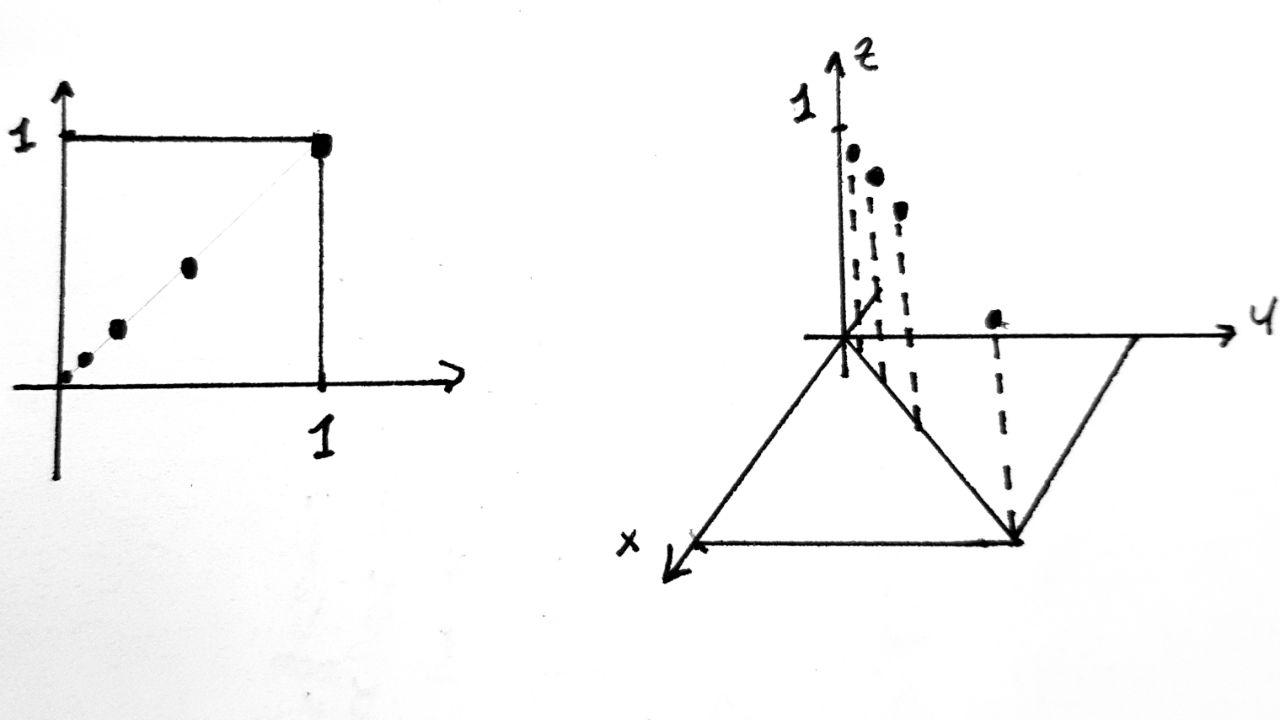
\includegraphics[width=93 mm,scale=1]{fig6.jpg}}
%\label{fig: }
%\end{figure}

\subsection{Integrazione in coordinate sferiche}

Le coordinate sferiche in $\mathbb{R}^3$ sono descritte dalla terna ($\rho, \theta , \phi$). Preso un punto $P=$($\rho, \theta , \phi$),  $\rho$ rappresenta il raggio della sfera, ovvero la distanza dall'origine di $P$, $\theta$ l'angolo descritto nel piano $x$-$y$, a partire dall'asse $x$ (analogamente alle coordinate polari in $\mathbb{R}^2$). Infine $\phi$ corrisponde all'angolo fatto partendo dall'asse $z$, nel piano contenente l'asse $z$ e $P$. Chiamiamo inoltre $r$ la distanza dall'origine della proiezione di $P$ nel piano $x$-$y$, allora chiaramente varrà $r=\rho \sin{\phi}$. Per il raggio deve valere $\rho >0$, invece scegliamo poi $\phi \in [0, \pi]$ e $\theta \in [0, 2\pi].$ 
\\ Passaggio di coordinate da sferiche a cartesiane
$$\vec{g} \left(\begin{matrix}  r \\ \theta \\ \phi  \end{matrix}\right) = \begin{bmatrix} x \\ y \\ z \end{bmatrix} = \begin{bmatrix} r \cos\theta \\ r \sin\theta \\ \rho \cos\phi \end{bmatrix}
 = \begin{bmatrix} 
 \rho \sin\phi \cos\theta \\ 
 \rho \sin\phi \sin\theta \\ 
 \rho \cos\phi 
 \end{bmatrix}$$.
%\begin{figure}[ht]
%\centering
%\centerline{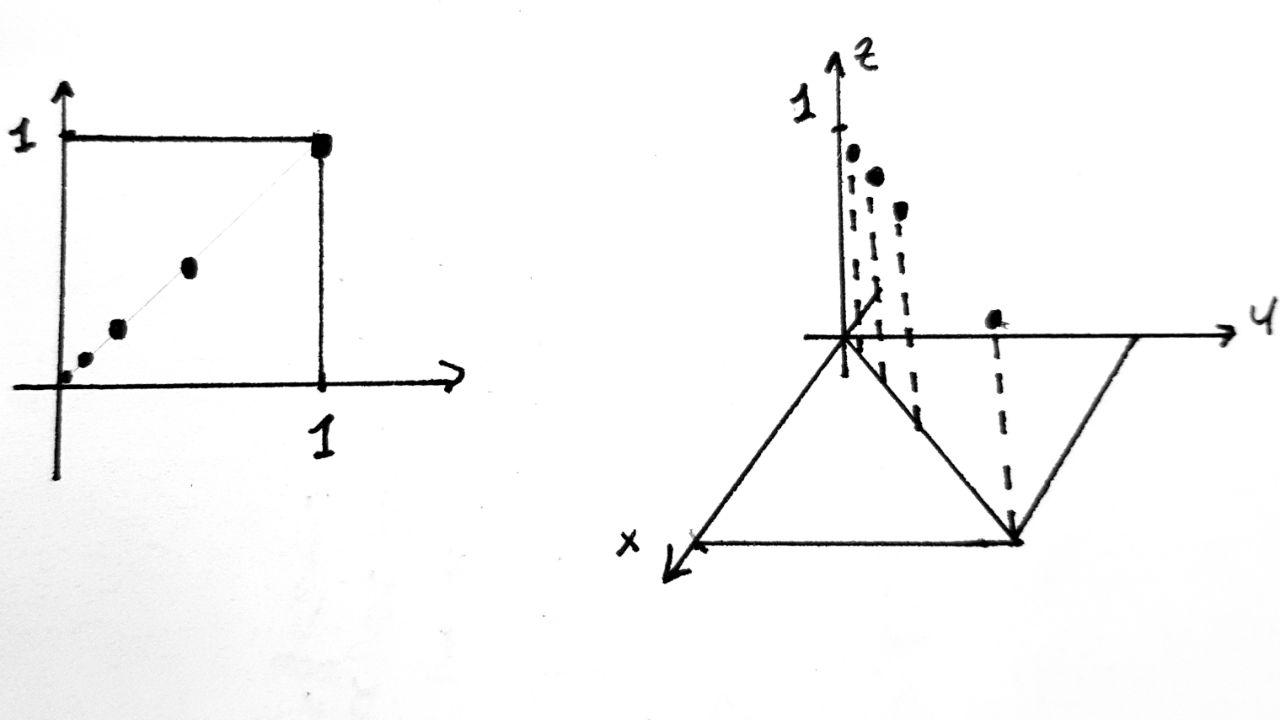
\includegraphics[width=93 mm,scale=1]{fig6.jpg}}
%\label{fig: }
%\end{figure}
\subsubsection{Esempio 0.}
Supponiamo di voler scrivere in coordinate sferiche l'equazione di una sfera di raggio $a$. Quando in cartesiane è $x^2+y^2+z^2=a^2$, per le sferiche vale semplicemente $\rho =a$, se non fosse chiaro intuitivamente basta sostituire all'interno dell'equazione cartesiana le formule di passaggio tra i due tipi di coordinate.

\subsubsection{Esempio 1.}
Vogliamo ora trovare l'equazione di una sfera di raggio $a$ traslata verso la parte positiva dell'asse $z$ di $a$. In coordinate cartesiane $x^2+y^2+(z-a)^2=a^2$. Il problema si può risolvere in due modi analogamente al caso bidimensionale con le coordinate polari. Quello più veloce è quello di notare che anche in questo caso presa un qualsiasi punto $P$ se effettuiamo una sezione della sfera passante per $P$ ed $O$, congiungendo $P$, e i 2 poli della sfera (i punti $(0, 0, -a)$ e $(0, 0, -a)$ in coord. cartesiane) otteniamo un triangolo rettangolo per cui vale $\rho = 2a\cos \phi$. Lo stesso risultato si trova mettendo a sistema le leggi per il passaggio di coordinate e l'eq. cartesiana.
\\ Notiamo inoltre che abbiamo trovato la stessa formula che descriveva la traslazione verso la parte positiva dell'asse $y$ di una circonferenza in $\mathbb{R}^2$. Potremmo allora azzardare l'ipotesi che se traslassimo la sfera verso l'asse $y$ anziché quello $z$ otterremmo l'equazione $\rho = 2a\sin \phi$, proprio come quando nel caso bidimensionale la traslazione veniva effettuata lungo l'asse $x$ anziché lungo $y$. Questo però è sbagliato perché non c'è la stessa simmetria visto che in questo caso abbiamo due angoli che oltretutto hanno domini differenti. L'equazione corretta in coordinate sferiche è $\rho=2a\sin \phi \sin{\theta}$.
\\
\begin{thm}
Data $S$ l'immagine di $\Omega \subset \mathbb{R}^3$ sotto la funzione $\vec{g}$, vale
$$\int_{\Omega} f(x,y,z)\ dV_{xyz} = \int_S (f\circ \vec{g}) (\rho, \phi, \theta) \rho^2 \sin{\phi} \ d\rho d\phi d\theta. $$
\end{thm}
Come nel caso in $\mathbb{R}^2$ con le coordinate polari, la prova a livello intuitivo si può visualizzare pensando di trasformare un volumetto infinitesimo di volume $d\rho \ d\phi \ d\theta$ in coordinate cartesiane. Allora $d\rho$ rimane tale e quale, la variazione di $\phi$ in coordinate cartesiane è un aumento di arco di circonferenza che vale $\rho d\phi$. Per $\theta$ vale la stessa cosa, solo che la variazione di $\theta$ è la variazione della proiezione sull'asse $x$-$y$, quindi il raggio della circonferenza di cui c'è un incremento di arco è $r = \rho \sin\phi$. 

\subsubsection{Esempio 2.}
Possiamo calcolarci facilmente il volume di una sfera piena di raggio $a$.
$$\int_{\Omega} 1\ dV_{xyz} = \int_0^{2\pi} \int_0^{\pi} \int_0^a  \rho^2 \sin{\phi} \ d\rho d\phi d\theta = 2\pi \int_0^{\pi} \sin \phi \ d\phi \int_0^{a} \rho ^2 = \frac{4}{3}\pi a^3. $$

\subsubsection{Esempio 3.}
Vogliamo calcolare il volume di $\Omega$, regione limitata da sopra dalla sfera $x^2+y^2+z^2=2$ e sotto dal cono $z=\sqrt{x^2+y^2}$.
$$\int_{\Omega} 1\ dV_{xyz} = \int_0^{2\pi} \int_0^{\frac{\pi}{4}} \int_0^{\sqrt{2}}  \rho^2 \sin{\phi} \ d\rho d\phi d\theta. $$

\section{Lezione del 12 Ottobre 2018}

\subsection{Applicazioni alla fisica di integrali di volume}
Immagino $\Omega \in \mathbb{R}^n$ come un corpo con determinate proprietà fisiche e spaziali.
\begin{defn}
Preso un cubetto $R_\varepsilon$ infinitesimo di lato $\varepsilon$ (rettangolo 3-dimensionale contenuto in $\Omega$) se $\vec{x}$ è il suo baricentro, definisco la sua \textit{densità} come
$$\delta(\vec{x})=\frac{massa(R_\varepsilon)}{vol_n(R_\varepsilon)}.$$ 
Per avere la densità puntuale in $\vec{x}$ mi basta fare il limite per $\varepsilon$ che tende a $0^+$.
\end{defn}
Dalla definizione segue che, se sono in un compatto rettificabile, vale
$$massa(\Omega)=\int_\Omega \delta \ dV. $$
Per la definizione di massa rimandiamo alla definizione data nel corso di Meccanica Analitica, staccandoci dalla definizione circolare data nel corso di Fisica Generale I.
\\ Prendiamo un corpo $\Omega$ di massa totale $M$ e lo circoscriviamo in un rettangolo 3-dimensionale, a questo punto prendiamo una partizione del rettangolo, suddividendo così il corpo in piccole regioni, che contraddistingueremo con l'indice $i$. In base a come viene scelta la partizione avremo diverse modi con cui vengono scelti i volumetti che compongono $\Omega$, chiameremo una configurazione discreta $C$.
\begin{defn}
Sia $C$ una configurazione discreta di $\Omega$, composta da $N$ volumetti di massa $m_i$ e posizione $\vec{x}_i$, con $i=1,...,N$. Definiamo la \textit{posizione del centro di massa di $\Omega$}
$$\vec{x}_{CM}=\langle \vec{x} \rangle_C = \frac{\sum_i^N m_i \vec{x} _i}{\sum_i^N m_i} = \frac{\sum m_i \vec{x} _i}{M}. $$
\end{defn}
Dalla definizione di densità si ha 
$$\vec{x}_{CM}= \frac{\sum_i^N (\delta_i \Delta V_i) \vec{x} _i}{(\delta_i \Delta V_i)}, $$ che passando al continuo diventa
$$\vec{x}_{CM}= \frac{\int_\Omega \delta \vec{x} \ dV }{\int_\Omega \delta\  dV }. $$
\\ Ricordiamo che data $f= [f_1, ... , f_n]$ funzione vettoriale, vale
$$\int_\Omega \vec{f} \ dV = 
\begin{bmatrix}
\int_\Omega f_1\ dV \\
\vdots \\
\int_\Omega f_n\ dV
\end{bmatrix}
.$$
Inoltre è sempre valida la proprietà
$$\left \Vert \int_\Omega \vec{f} \ dV \right \Vert \leq \left \vert \int_\Omega ||\vec{f} || dV \right \vert . $$

\subsubsection{Esempio 1.}
Come esempio vediamo di trovare il centro di massa della semisfera $B(\vec{0}, a)/2$, in cui la densità è proporzionale al quadrato della distanza dall'origine ($\delta (\vec{x})= k ||\vec{x}|| ^2$). Prendiamo la semisfera tagliata dall'asse $x$-$y$ e consideriamo la parte positiva dell'asse $z$. Chiaramente $\Omega$ e $\delta$ sono simmetriche rispetto all'asse delle $z$, avremo $\vec{x}_{CM}=(0,0,z_{CM})$.
Risolviamo 
$$z_{CM}= \frac{\int_\Omega \delta z \ dV }{\int_\Omega \delta\  dV }. $$
Per il denominatore, passando in coordinate sferiche (per le quali $\delta= k \rho ^2$):
$$M= \int_\Omega \delta\  dV = k \int_0^{2\pi} \int_0^{\frac{\pi}{2}} \int_0^a \rho^2\ \rho^2 \sin\phi \ d\rho d\phi d\theta= k \frac{2}{5}\pi a^5.$$
A nominatore invece abbiamo
$$\int_\Omega \delta\ z\ dV = k \int_0^{2\pi} \int_0^{\frac{\pi}{2}} \int_0^a \rho^2\ (\rho \cos\phi) \rho^2 \sin\phi \ d\rho d\phi d\theta= k \frac{\pi}{6} a^6.$$
Quindi 
$$z_{CM}= \frac{\frac{\pi}{6}a^6}{\frac{2}{5}\pi a^5}= \frac{5}{12} a,$$ notiamo \textit{en passant} che se la densità fosse stata semplicemente proporzionale alla distanza allora si avrebbe avuto $z_{CM}=2/5a$.
\\
\\
\textbf{Momento di inerzia}\\
L'energia cinetica di traslazione di una particella è data da $T=\frac{1}{2}m\lVert\vec{v}\rVert^2$.\\
Se la particella oltre a traslare, ruota anche attorno ad un asse a distanza $R_i$ ad una velocità $\lVert \vec{v} \rVert = R_i \omega$, questa possiederà anche una energia cinetica di rotazione. Se si considera un sistema di particelle allora l'energia cinetica totale sarà la somma delle singole energie possedute dalle particelle, quindi si scriverà:
$$T=\sum_i \frac{1}{2}m_i\lVert\vec{v}_i\rVert^2 = \sum_i \frac{1}{2}m_i(\omega R_i)^2 = \frac{1}{2} \underbrace{\left( \sum_i m_i R_i^2\right)}_{I}\omega^2 = \frac{1}{2} I \omega^2$$
$I=\sum_i m_i R_i^2$ è il momento di inerzia, rappresenta l'inerzia di un corpo per le rotazioni. Può essere applicato ai corpi solidi che non sono altro che sistemi di particelle con una geometria ben precisa, in cui le distanze tra le particelle non cambiano nel tempo. Dalla definizione si può intuire che il momento di inerzia non dipende solo dalla massa ma anche da come questa è distribuita rispetto all'asse di rotazione. Dalla versione discreta se si passa al continuo:
$$I=\int_{\Omega} \delta(\vec{r})\, dist(\vec{x},AS)^2 \,dV$$
dove $\delta(\vec{r})$ è la densità di massa e con $AS$ si indica l'asse di rotazione. Inoltre nell'integrale si è sostituita una massa infinitesima con la densità di massa ed il volume infinitesimo $dm = \delta(\vec{r}) \,dV$.

\subsubsection{Esempio 2.}
Da un piano inclinato sono fatti rotolare in condizione di rotolamento puro cinque corpi solidi (un anello, una palla piena, una palla cava, un cilindro pieno e un doppio cono), tutti con raggio massimo $a$ e tutti con la medesima massa $m$. Quale è il solido che giunge prima in fondo al piano inclinato?\\ 
\\
Dalla conservazione dell'energia e dalla condizione di rotolamento puro $\lVert \vec{v} \rVert = R_i \omega$ si può ricavare la velocità finale posseduta dai corpi.
$$mgh = \frac{1}{2}m \lVert \vec{v} \rVert^2 + \frac{1}{2} I \omega^2 = \frac{1}{2}m \lVert \vec{v} \rVert^2 + \frac{1}{2} I \frac{\lVert \vec{v} \rVert^2}{a^2} = \frac{1}{2} \left( 1+\frac{I}{ma^2}\right)m\lVert \vec{v} \rVert^2$$
$$\Rightarrow gh = \frac{1}{2} \left( 1+\frac{I}{ma^2}\right)\lVert \vec{v} \rVert^2$$
A questo punto si vede bene che la velocità finale con cui arrivano i corpi in fondo non dipende dalla loro massa, infatti il termine $\frac{I}{ma^2}$ è un numero puro. Noi vogliamo trovare quale è il corpo che arriverà prima, che si traduce anche con il dire quale corpo avrà la velocità massima in fondo al piano inclinato, quindi il corpo che avrà $\frac{I}{ma^2}$ minimo sarà quello che cerchiamo ($I$ va calcolato rispetto all'asse di rotazione passante per il centro di massa del solido).
\begin{itemize}
    \item \textit{Anello.}\newline
Tutta la massa è distribuita alla stessa distanza dall'asse di rotazione
$$I=ma^2 \Rightarrow \frac{I}{ma^2}=1$$
    \item \textit{Cilindro pieno.}\\
Già calcolata precedentemente
$$I=\frac{1}{2}ma^2 \Rightarrow \frac{I}{ma^2}=\frac{1}{2}$$
\item \textit{Sfera piena.}\\
Conviene svolgere l'integrale triplo in coordinate sferiche quindi prendendo la $dist(\vec{x},AS) = \rho \sin \phi$
$$I = \int_0^{2\pi}\int_0^{\pi}\int_0^a \delta(\vec{r})(\rho\sin\phi)^2\rho^2\sin\phi \,d\rho \,d\phi \,d\theta = 2 \pi \frac{a^5}{5} \frac{4}{3} \delta = \frac{8}{15} \pi a^5 \delta $$
$$\Rightarrow I=\frac{2}{5}\left( \frac{4}{3} \pi  a^3 \delta\right)a^2 \Rightarrow \frac{I}{ma^2}=\frac{2}{5}$$
\item \textit{Sfera cava.}\\
Si trova il momento di inerzia della palla di raggio $a$ e si sottrae a questo quello relativo ad una palla di raggio minore $b$, poi si fa tendere $b \to a$. 
$$I=\frac{2}{3}ma^2 \Rightarrow \frac{I}{ma^2}=\frac{2}{3}$$
\item \textit{Doppio cono.}\\
Conviene svolgere l'integrale triplo in coordinate cilindriche quindi prendendo la $dist(\vec{x},AS) = r$. Calcoliamo prima il momento di inerzia di uno solo dei due coni. Sfruttiamo le proprietà dei triangoli simili per ottenere le relazioni $\frac{z}{r} = \frac{h}{a} \Rightarrow z=r\frac{h}{a}$.
$$I = \int_0^{2\pi}\int_0^{a}\int_{r\frac{h}{a}}^h \delta(\vec{r})\,r^2 \cdot r \,dz \,dr \,d\theta = \delta \frac{\pi}{10} h a^4$$
$$\Rightarrow I=\frac{3}{10}\left( \frac{1}{3} \pi h a^2 \delta\right)a^2 \Rightarrow \frac{I}{ma^2}=\frac{3}{10}$$
\end{itemize}
Quindi il doppio cono è il solido di rotazione che arriverà per primo in fondo al piano.

\section{Lezione del 17 Ottobre 2018}
\begin{defn}
$A, B \subset \mathbb{R}^n$ aperti. Chiameremo $\vec{g}:A\to B$ un \textbf{cambiamento di variabili} se
\begin{enumerate}
    \item $\vec{g}$ è iniettiva;
    \item $\vec{g}$ è (almeno) $\mathcal{C}^1$;
    \item la matrice Jacobiana $D\vec{g} \in Aut(\mathcal{R}^n)$ è invertibile.
\end{enumerate}
\end{defn}

\textit{Osservazione:}
\\ Ogni diffeomorfismo (funzione bigettiva, $\mathcal{C}^1$ e con inversa $\mathcal{C}^1$) è equivalente ad un cambio di variabili.

\begin{thm}
(del cambiamento di variabili) Sia $\Omega \subset \mathbb{R}^n$ compatto rettificabile e $A$ aperto con $\Omega \subset A$. Sia $\vec{g}:A\to \mathbb{R}^n$ un cambio di variabili. Se $S=\vec{g}(\Omega)$ e $f:S\to \mathbb{R}$ integrabile allora vale 
$$\int_{\Omega} (f\circ \vec{g})(\vec{u})\ |det(D\vec{g}(\vec{u}))|\ dV_{\vec{u}}=\int_Sf(\vec{x}) dV_{\vec{x}}.$$
\end{thm}
\bigskip


\subsubsection{Esempio 1.}
Vogliamo calcolare la superficie di una funzione nel dominio $S$, ovvero un'ellisse di equazione $\frac{x^2}{4}+y^2\leq 1$. 
Un utile cambio di variabili potrebbe essere quello delle polari:
$$
\vec{g}\left(\begin{matrix}  r \\ \theta  \end{matrix}\right)=
\begin{bmatrix}
r\cos \theta \\ r\sin \theta
\end{bmatrix}
$$
e la matrice Jacobiana
$$
D\vec{g}=
\begin{bmatrix}
\cos \theta & -r\sin\theta \\ \sin \theta & r\cos\theta
\end{bmatrix}
\Longrightarrow det(D\vec{g})=r\qquad \quad con\ r>0.
$$
Applicando $\vec{g}$ ad un dominio $\Omega$ quadrato (nelle coordinate polari) però otteniamo una circonferenza in coordinate cartesiane. 
Per ottenere un'ellisse possiamo utilizzare un cambiamento di variabili 
$$T
\begin{bmatrix}
u \\ v
\end{bmatrix}
=
\begin{bmatrix}
2u \\
v
\end{bmatrix}\Longrightarrow T = 
\begin{bmatrix}
2 & 0\\ 0 & 1
\end{bmatrix}
\begin{bmatrix}
u \\ v
\end{bmatrix}$$
e comporlo con $\vec{g}$ per creare un'unico cambiamento di variabili $T\circ \vec{g}$ che partendo da un dominio $\Omega$ di facile integrazione arriva al dominio $S$ di partenza.
Chiamata $f$ la funzione di cui vogliamo calcolare la superficie avremo quindi
$$\int_Sf\ dA_{xy} = \int_{\Omega}f\circ(T\circ \vec{g})(r, \theta) \ |det(D(T\circ \vec{g})(r,\theta))|\ dV_{(r,\theta)}.
$$
Notiamo \textit{en passant} che essendo $T$ una funzione lineare vale
$$det(D(T\circ \vec{g}) = (det(T))(det(D\vec{g}))=(2)(r)= 2r
$$

\subsubsection{Esempio 2.}
Dato $S$ il dominio di integrazione definito come l'area tra le rette:\\
$x+y=0 \quad x+y=3 \quad y=2x \quad y=2x+1$, calcolare l'integrale
$$\int_S \frac{2x-y}{x+y+4} \,dA_{xy}$$
Per risolvere questo integrale si può procedere facendo un opportuno cambio di variabili, ad esempio
$$\begin{cases}
 u = 2x-y \\ v=x+y+4
\end{cases}$$
Da notare che questo non è l'unica sostituzione possibile, funziona con tutte le sostituzioni, ma lo scopo di questo metodo di risoluzione è quello di semplificare il calcolo dell'integrale, quindi è bene scegliere un cambio di coordinate(variabili) furbo ed ottimale.\\
In più bisogna fare attenzione che il sistema scritto sopra non rappresenta la funzione $\vec{g}$, ma piuttosto la sua inversa.
$$\vec{g} \left( \begin{matrix} u \\ v \end{matrix}\right) = \begin{bmatrix} x\\ y \end{bmatrix} \qquad \Leftrightarrow \qquad \vec{g}^{-1} \left( \begin{matrix} x \\ y \end{matrix}\right) = \begin{bmatrix} u\\ v \end{bmatrix} $$
Quindi trovo la matrice che rappresenta l'inversa di $\vec{g}$, facendo attenzione che si tratta di una trasformazione affine e non vettoriale (dovuta alla presenza del "$+4$")
$$\Rightarrow \begin{bmatrix} 2 & -1 \\ 1 & 1  \end{bmatrix} \begin{bmatrix} x \\ y \end{bmatrix} = \begin{bmatrix} u \\ v-4  \end{bmatrix}$$
Ora sapendo che il cambio di coordinate è un diffeomorfismo allora posso trovare la matrice di $g$ invertendo la matrice che rappresenta la sua inversa.
$$\begin{bmatrix} x \\ y  \end{bmatrix} = \begin{bmatrix} 2 & -1 \\ 1 & 1  \end{bmatrix}^{-1} \begin{bmatrix} u \\ v-4 \end{bmatrix} = \frac{1}{3} \begin{bmatrix} 1 & 1 \\ -1 & 2  \end{bmatrix} \begin{bmatrix} u \\ v-4 \end{bmatrix} = \frac{1}{3} \begin{bmatrix} u+v-4 \\ -u +2v -8  \end{bmatrix}$$
Giunti a questo punto si può applicare il teorema di cambio di variabile
$$\int_S \frac{2x-y}{x+y+4} \,dA_{xy} = \int_{\Omega} \frac{u}{v} | \det \overbrace{D\vec{g}(\vec{u})}^{\vec{g}(\vec{u})}| \,dV_{uv} $$
Una volta calcolato il determinante della matrice, quindi
$$\det \left(\frac{1}{3} \begin{bmatrix} 1 & 1 \\ -1 & 2  \end{bmatrix}\right) = \left( \frac{1}{3}\right)^2 \cdot 3 = \frac{1}{3}$$
si può passare al calcolo esplicito dell'integrale
$$=\int_{\Omega} \frac{u}{v} \left(\frac{1}{3}\right) \,dV_{uv} = \frac{1}{3}\int_4^7\int_{-1}^0 \frac{u}{v}\,du\,dv = \frac{1}{3} \left( -\frac{1}{2}\right) \log \frac{7}{4}$$
L'integrale è negativo quindi in quel intervallo di definizione la funzione è per lo più negativa.
\\

%\begin{figure}[ht]
%\centering
%\centerline{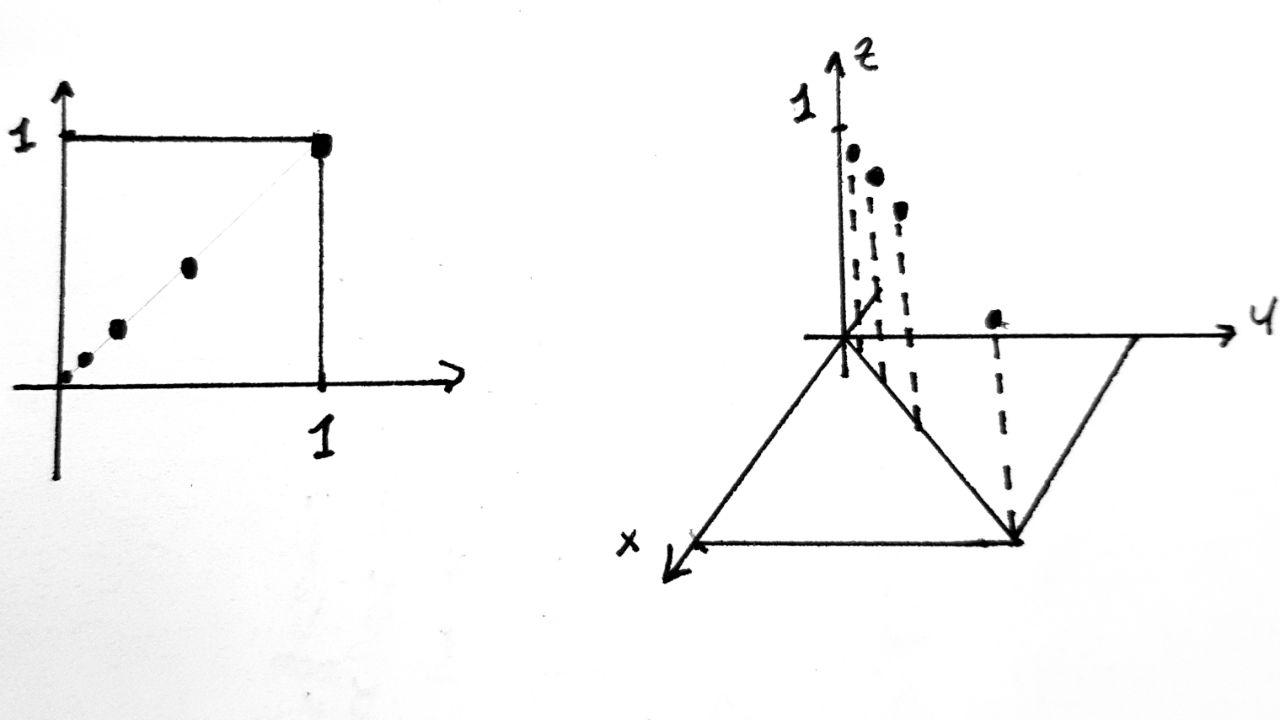
\includegraphics[width=93 mm,scale=1]{fig6.jpg}}
%\label{fig: }
%\end{figure}

\subsubsection{Esempio 3.}
Risolviamo lo stesso integrale di superficie dell'esercizio precedente, questa volta utilizzano come intervallo di definizione quello definito dalle rette \\ $y=2x \quad x+y=0 \quad x=2$.
$$x=2 \qquad \Leftrightarrow \qquad \frac{1}{3}(u+v-4) =2 \qquad \Leftrightarrow \qquad u+v=10$$
$$\int_S \frac{2x-y}{x+y+4} \,dA_{xy} = \int_{\Omega} \frac{u}{v}\,dA_{uv} = \frac{1}{3} \int_4^{10} \int_0^{10-v} \frac{u}{v} \,du\,dv$$

%\begin{figure}[ht]
%\centering
%\centerline{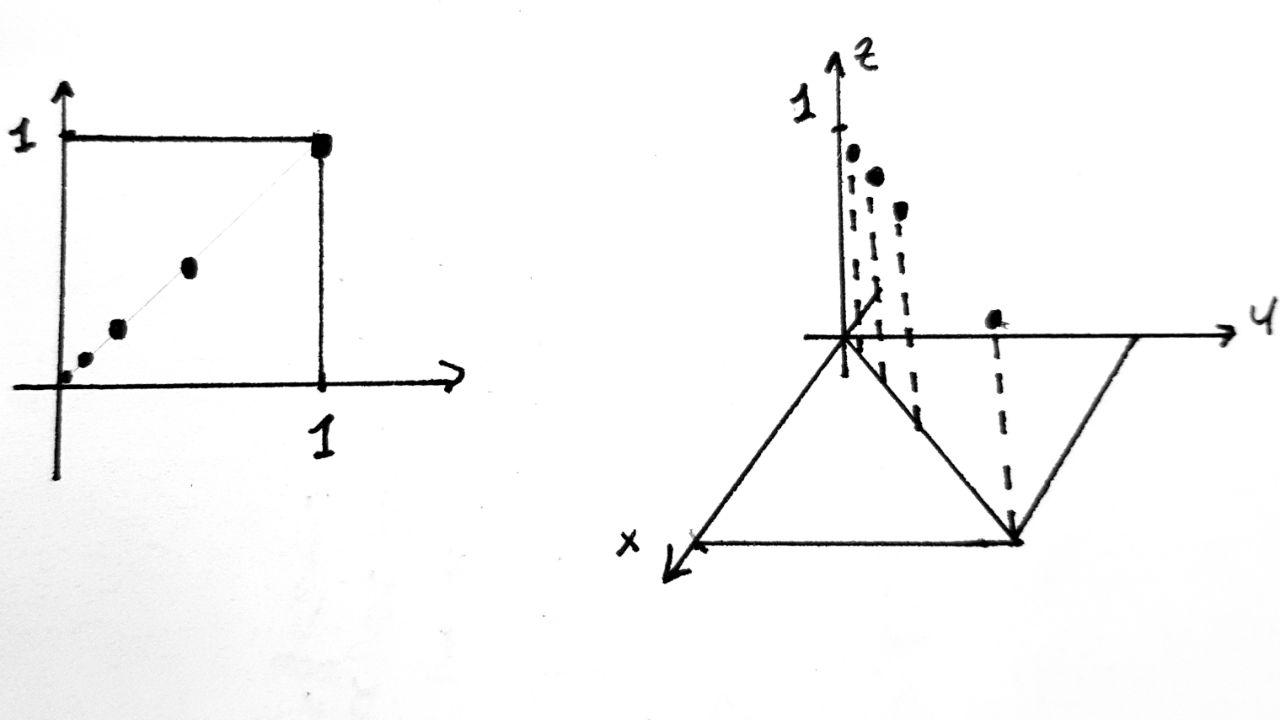
\includegraphics[width=93 mm,scale=1]{fig6.jpg}}
%\label{fig: }
%\end{figure}

\subsubsection{Esempio 4.}
Sia $\vec{f}$ e sia $S$ l'intervallo di definizione definito dalle funzioni \\
$xy=1 \quad xy=3 \quad y=x \quad y=2x^2$.
$$\vec{g} \left( \begin{matrix} u \\ v \end{matrix}\right) = xy$$
In coordinate cartesiane è possibile risolverlo ma risulta molto complicato, quindi facciamo un cambio di variabili\\
$$\begin{cases}
 u = xy \\ v=\frac{y}{x} \quad oppure \quad \frac{x}{y}
\end{cases}$$
Partiamo dalla retta e la scegliamo in modo da semplificare anche $y=2x^2$.\\
Dobbiamo cercare la iniettività, quindi se trovo $-Id$ come trasformazione (come in questo caso) significa che non c'è iniettività, però qui abbiamo $x,y>0$, perciò mi posso restringere in questo intorno dove abbiamo iniettività. \\
Di seguito sono riportate tutte le relazioni per il cambio di variabili.
$$
se \; x,y>0 \qquad \Rightarrow \qquad
\begin{cases}
 x=\sqrt{\frac{u}{v}} \\ y=\sqrt{uv}
\end{cases}
$$
$$
\vec{g} \left( \begin{matrix} u \\ v \end{matrix}\right) = \begin{bmatrix} x\\ y \end{bmatrix} \qquad \Leftrightarrow \qquad \vec{g} \left( \begin{matrix} u \\ v \end{matrix}\right) = \begin{bmatrix} \sqrt{\frac{u}{v}}\\ \sqrt{uv} \end{bmatrix} $$

$$ D\vec{g} \begin{bmatrix} \frac{1}{2\sqrt{uv}} & -\frac{1}{2} \sqrt{u} v^{-\frac{3}{2}}\\ \frac{1}{2} \sqrt{\frac{v}{u}} & \frac{1}{2} \sqrt{\frac{u}{v}} \end{bmatrix} \qquad \det D\vec{g} \left( \begin{matrix} u \\ v \end{matrix} \right) = \frac{1}{4v} + \frac{1}{4v} = \frac{1}{2v}$$

$$y=2x^2 \qquad \Leftrightarrow \qquad \sqrt{uv} = 2 \frac{u}{v} \qquad \Leftrightarrow \qquad u = \frac{1}{4} v^3 $$
\\
Dopo aver fatto tutte le sostituzioni con le relazioni precedenti, l'integrale sarà:
$$\int_S xy \,dA_{xy} = \int_{\Omega} u \; |\det D\vec{g}| \, dA_{uv} = \frac{1}{2} \int_{\Omega} \frac{u}{v} \,dA_{uv}$$
$$ = \frac{1}{2} \int_1^3 \int_1^{(4u)^{\frac{1}{3}}} \frac{u}{v} \,dv\,du = \dots =\frac{2}{3} \log 4 +\frac{3}{4} \log 3 - \frac{1}{3}$$



\section{Lezione del 19 Ottobre 2018}
Prima di vedere gli integrali curvilinei ricordiamo che data una funzione $\vec{g}:\mathbb{R}^n \to \mathbb{R}^n$ invertibile ($\vec{g}^{-1} \circ g = id_{\mathbb{R}^n}$), vale per la regola della catena 
$$D\vec{g}^{-1}(\vec{g}(\vec{x})) \cdot D\vec{g}(\vec{x}) = 
\mathbbm{1} \Longrightarrow det(D\vec{g}^{-1} \circ \vec{g}) = \frac{1}{det(D\vec{g})}.
$$
\subsection{Integrali curvilinei}
\begin{defn}
Data $\vec{\gamma}:I\to \mathbb{R}^2$ curva piana parametrizzata con $I\in \mathbb{R}$, $\vec{\gamma}\in \mathcal{C}^1(I,\mathbb{R}^2)$, $\vec{\gamma}'(t)\neq \vec{0},\ \forall t \in I=[a, b]$ intervallo regolare. Chiamo $C$ una curva regolare in $\mathcal{R}^2$.
Allora data una funzione $f:A\to \mathbb{R},\ A \in \mathbb{R}^2$ aperto, definiamo
$$
\int_Cf\ ds \doteq \int_a^b(f\circ\vec{\gamma})(t)\ ||\vec{\gamma}'(t)||_{\mathbb{R}^2}\ dt.
$$
\end{defn}
\bigskip
A partire dalla definizione diremo che la "lunghezza" di $C$ è
$$l(C)=\int_C ds = \int_a^b||\vec{\gamma}'(t)||_{\mathbb{R}^2}\ dt.$$
\\ Per la linearità dell'integrale se la curva $C$ è formata da $N$ curve differenti ($C=\bigcup_{i=1}^NC_i$) vale
$$l(C)=\int_C f\ ds = \sum_{i=1}^N\int_{C_i}f\ ds.$$

\subsubsection{Esempio 1.}
Valutare l'integrale $\int_C(x^2y+2)\ ds$ dove $C$ è la semicirconferenza superiore della cirocnferenza unitaria.
\\ La parametrizzazione ovvia da fare è
$$\vec{\gamma}(t)=\left( \begin{matrix}x(t) \\ y(t) \end{matrix} \right) 
= \left( \begin{matrix} \cos(t) \\ \sin(t) \end{matrix} \right), \qquad t\in [0, \pi]. 
$$
Applichiamo la definizione
$$\int_C(x^2y+2)\ ds \doteq \int_0^{\pi}(cos^2(t)sin(t)+2)\ \sqrt{cos^2(t)+sin^2(t)}\ dt =[\frac{1}{3}cos^3(t)]_0^\pi+[2t]_0^\pi=-\frac{2}{3}+2\pi.$$.
\subsubsection{Esempio 2.}
Valutare l'integrale $\int_Cy\sqrt{1+4x^2}\ ds$ dove $C$ è la parte di parabola $y=x^2$ con $x\in [-1,1]$. Ma notiamo che $C$ è il grafico di una funzione, in questo caso quindi
$$\vec{\gamma}(t)=\left( \begin{matrix}x(t) = t \\ y(t) = t^2 \end{matrix} \right) 
$$
e di conseguenza
$$\vec{\gamma}'(t)=\left( \begin{matrix}1 \\ 2t \end{matrix} \right) \Longrightarrow ||\vec{\gamma}'(t)||=\sqrt{1+4t^2}
$$.
Applichiamo la definizione
$$\int_Cy\sqrt{1+4x^2}\ ds=\int_{-1}^1t^2\sqrt{1+4t^2}\ \sqrt{1+4t^2}\ dt =
\int_{-1}^1 t^2+4t^4\ dt = \frac{34}{15}
$$

\subsubsection{Esempio 3.}
Valutare l'integrale $\int_Cxy\ ds$ dove $C$ è il bordo del quadrato $[0,1]\times [0,1]$. Possiamo chiamare $C_1$ il lato che congiunge gli estremi $(0,0)$ e $(1,0)$, $C_2$ il lato che congiunge $(1,0)$ e $(1,1)$, $C_3$ il lato che congiunge $(1,1)$ e $(0,1)$ e $C_4$ il lato che congiunge gli estremi $(0,1)$ e $(0,0)$. Si ha quindi $\int_Cxy\ ds=\sum_{i=1}^4\int_{C_i}xy\ ds$.
Possiamo parametrizzare facilmente:
$$ \vec{\gamma}_1=\begin{bmatrix}t\\0 \end{bmatrix}; \ \
\vec{\gamma}_2=\begin{bmatrix}1\\t \end{bmatrix};\ \
\vec{\gamma}_3=\begin{bmatrix}1-t\\1 \end{bmatrix};\ \
\vec{\gamma}_4=\begin{bmatrix}0\\1-t \end{bmatrix};\qquad per\ t\in [0,1].
$$
Notiamo subito che i contributi all'integrale dati da $C_1$ e $C_4$ sono nulli poiché la funzione da integrare è $f=xy$, e $\vec{\gamma}_1$ e $\vec{\gamma}_4$ hanno una componente nulla.
Per $C_2$ e $C_3$ invece
$$\vec{\gamma}_2'=\begin{bmatrix}0\\1 \end{bmatrix} \Rightarrow ; \ \
\vec{\gamma}_3'=\begin{bmatrix}-1\\0 \end{bmatrix}; ||\vec{\gamma}_{2,3}'(t)|| = 1.
$$
Quindi
$$\int_Cxy\ ds=\sum_{i=1}^4\int_{C_i}xy\ ds= \int_0^1(1t)(1)\ dt + \int_0^1(1(1-t))(1)\ dt = 1.$$


\section{Lezione del 24 Ottobre 2018}
 
\subsubsection{Esercizio 1.}
Calcolare l'area della superficie del cilindro retto $x^2+y^2=1$ compresa tra i piani $z=0 \quad z+y=2$.
$$z= f(x,y) = 2-y \qquad f \text{ definita su } x^2+y^2=1 \quad \Leftarrow \quad C$$
$$Area(S) = \int_C (2-y)\,dS$$
Troviamo una parametrizzazione 
$$\vec{r}(t)= \begin{bmatrix} \cos t \\ \sin t \end{bmatrix} \qquad \vec{r}\,'(t)= \begin{bmatrix} - \sin t \\ \cos t \end{bmatrix} \qquad \| \vec{r}\,'(t) \| = 1 \qquad t \in [0,2\pi]$$
$$\int_C (2-y)\,dS = \int_0^{2 \pi} (2-y) (\vec{r}(t)) \cdot \| \vec{r}\,'(t) \| \,dt = \int_0^{2 \pi} (2- \sin (t))\,dt = 4 \pi$$
\\
Integrazione sulle componenti
\\
$$\int_C f\,ds \simeq \sum_i f(\vec{x}_i , \vec{y}_i)\,ds_i $$
Integro sulle componenti, ovviamente otterrò integrali con il segno (derivate versori). Se integro sulla curva ottengo il modulo.
$$\int_C f\,dx \doteq \int_a^b (f \circ \vec{r})(t) x'(t) \,dt $$
$$ \int_C f\,dy \doteq \int_a^b (f \circ \vec{r})(t) y'(t) \,dt$$
Prendiamo due punti P e Q su una traiettoria curvilinea e sviluppiamo l'integrale curvilineo rispetto alle sue componenti.
$$\int_C P(x,y)\,dx + \int_C Q(x,y)\,dy$$
$$\int_C P\,dx + \int_C Q\,dy = \int_a^b ((P \circ \vec{r})(t)x'(t) + (Q \circ \vec{r})(t)y'(t))\,dt$$

\subsubsection{Esercizio 2.}

Calcolare l'integrale $\int_C x^2 \,dx + y^2 \,dy$, dove C è l'arco di circonferenza tra i punti (2,0) e (0,2) e il segmento di retta tra i punti (0,2) e (4,3).
$$\int_C x^2 \,dx + y^2 \,dy = \int_{C1} x^2\,dx +y^2 \,dy + \int_{C2} x^2 \,dx + y^2 \,dy$$

$$C1 \Rightarrow \vec{r}_1(t) = \begin{bmatrix} 2\cos t \\ 2\sin t \end{bmatrix} \quad \vec{r}_1 \,' (t) = \begin{bmatrix} -2\sin t \\ 2\cos t \end{bmatrix} = \begin{bmatrix} x'(t) \\ y'(t)\end{bmatrix} \quad \| \vec{r}\,'(t) \| = 2 \quad t \in [0,2\pi]$$

$$\int_{C1} x^2\,dx +y^2\,dy = \int_0^{\pi/2} [4\cos ^2 t \cdot (-2\sin t) + 4\sin ^2 t \cdot (2\cos t)]\,dt =$$
$$= 8 \int_0^{\pi/2} [\sin ^2 t \cos t - \cos ^2 t \sin t]\,dt = 8 \left[ \frac{\sin ^3 t}{3} \right]_{t=0}^{t=\pi/2} +8 \left[ \frac{\cos ^3 t}{3} \right]_{t=0}^{t=\pi/2} = 8 \left( \frac{1}{3} - \frac{1}{3}\right) = 0$$
Questo integrale non contribuisce.\\
Facciamo una parametrizzazione per segmenti.
$$C2 \Rightarrow \vec{r}_2 (t) = (1-t) \begin{bmatrix} 0 \\ 2\end{bmatrix} +t \begin{bmatrix} 4 \\ 3\end{bmatrix} \qquad \vec{r}_2 \,' (t) = \begin{bmatrix} 4t \\ 2+t\end{bmatrix}' = \begin{bmatrix} 4 \\ 1\end{bmatrix} \qquad t \in [0,1] $$

$$\int_{C2} x^2 \,dx + y^2 \,dy = \int_0^1 [16t^2 \cdot 4 + (2+t)^2 \cdot 1]\,dt = \frac{83}{3}$$

\subsubsection{Esercizio 3.}

Utilizzo due parametrizzazioni diverse, ma con velocità uguale
$$\vec{r}_1 (t) = \begin{bmatrix} \cos t \\ \sin t\end{bmatrix} \qquad \vec{r}_1\,' = \begin{bmatrix} -\sin t \\ \cos t\end{bmatrix} \qquad t \in [0,\pi] \qquad \text{antiorario}$$

$$\vec{r}_2 (t) = \begin{bmatrix} -\cos t \\ \sin t\end{bmatrix} \qquad \vec{r}_2\,' = \begin{bmatrix} \sin t \\ \cos t\end{bmatrix} \qquad t \in [0,\pi] \qquad \text{orario}\quad \;\;$$

$$\int_C y\,ds$$
$$\vec{r}_1 \qquad \int_C y\,ds = \int_0^{\pi} \sin t \,dt =[ -\cos t ]_0^{\pi} =2$$
$$\vec{r}_2 \qquad \int_C y\,ds = \int_0^{\pi} \sin t \,dt =[ -\cos t ]_0^{\pi} =2$$
Una curva parametrizzata diversamente mi porta allo stesso risultato, questo non dipende dalla parametrizzazione.

$$\int_C x^2\,dx$$
$$\vec{r}_1 \qquad \int_C x^2\,dx = \int_0^{\pi} \cos ^2 t (-\sin t) \,dt =\left[ \frac{\cos ^3 t}{3} \right]_0^{\pi} =\frac{2}{3}$$
$$\vec{r}_2 \qquad \int_C x^2\,dx = \int_0^{\pi} \cos ^2 t (\sin t) \,dt =\left[ -\frac{\cos ^3 t}{3} \right]_0^{\pi} =-\frac{2}{3}$$
Integrali di linea di coordinate dipendono dalla parametrizzazione, dall'orientamento della curva, al contrario degli integrali curvilinei.

\subsection{Orientamento di una curva}
\begin{defn}
$\vec{r}:[a,b]\to \mathbb{R}^2$ parametrizzazione di una curva. Presi $t_1, t_2 \in [a,b]$, diremo che $P_1=\vec{r}(t_1)$ \textit{precede} $P_2=\vec{r}(t_2)$ se $t_1<t_2$.
\end{defn}
Il concetto di precedenza è fondamentale nel calcolo degli integrali curvilinei poiché una stessa curva (o supporto) $C$ può essere percorsa in due direzioni (che chiameremo $-C$ e $+C$). 
\\ In due dimensioni è presente una convenzione che distingue se la curva venga percorsa in senso positivo o negativo. Data una curva in $\mathbb{R}^2$ fissata una terna cartesiana $(\mathbf{e_1}, \mathbf{e_2}, \mathbf{e_3})$ destrorsa di modo che la curva stia nel piano individuato da $\mathbf{e_1}$ ed $\mathbf{e_2}$. Chiamiamo il vettore tangente alla curva $\vec{r}$:
$$\vec{\tau}(t)=\sum_{i=1}^3\frac{r'_i(t)}{||r'_i(t)||}\mathbf{e_i}=\begin{bmatrix}
\frac{r_1'(t)}{\sqrt{r_1'^2(t)+r_2'^2(t)}}
\\
\frac{r_2'(t)}{\sqrt{r_1'^2(t)+r_2'^2(t)}}
\\
0
\end{bmatrix}.
$$
Il vettore normale allora sarà
$$\vec{n}(t)=\begin{bmatrix}
\frac{r_2'(t)}{\sqrt{r_1'^2(t)+r_2'^2(t)}}
\\
-\frac{r_1'(t)}{\sqrt{r_1'^2(t)+r_2'^2(t)}}
\\
0
\end{bmatrix}.
$$
Ora diremo che la curva ha orientazione positiva se la terna ortonormale $(\vec{n}, \vec{\tau}, \mathbf{e_3})$ è destrorsa.

\subsection{Domini normali regolari}
\begin{defn}
Chiamremo $D\subset \mathbb{R}^2$ un \textit{dominio normale regolare} se è del tipo $D={(x,y):x\in[a,b], \alpha(x)\leq y \leq \beta(x)}$ con $\alpha, \beta:[a,b]\to \mathbb{R}$ di classe $\mathcal{C}^1$ e $\alpha(x)<\beta(x),\ \forall x\in[a,b]$.
\end{defn}
\bigskip
\textit{Osservazione:}
\\ Dalla definizione si ha che la frontiera di $D$, che in $n$ dimensioni viene detta bordo ($\partial D$), è sempre unione di un numero finito di curve regolari a tratti. Pertanto essa ammette versore tangente e versore normale in ogni suo punto, tranne al più un numero finito. Si definisce per convenzione orientamento positivo della frontiera il verso di percorrenza che lascia il versore normale in ogni momento esterno al dominio (o equivalentemente, che lascia il dominio sulla sinistra). Tale orientamento si indica con $ +\partial D$.
\\
Provvediamo ora ed ununciare importanti teoremi e formule di integrazione.
\begin{thm}
(di Gauss-Green)
Sia $D$ dominio regolare in $\mathbb{R}^2$ e $f$ una funzione definita in $D$ di classe $\mathcal{C}^1$, allora valgono
$$\int_D\frac{\partial f}{\partial x}\ dA = \int\displaylimits_{+\partial D}f\ dy;\qquad \qquad   \int_D\frac{\partial f}{\partial y}\ dA = -\int\displaylimits_{+\partial D}f\ dx.
$$
\end{thm}
\bigskip
Un semplice e immediato esempio di applicazione è quello per il calcolo dell'area del dominio $D$, ovvero
$$\int_D1\ dA. $$ Possiamo vedere $1$ come derivata parziale in $x$ o in $y$ delle funzioni rispettivamente $f\doteq x$ o $f\doteq y$.
Per il terorema appena visto allora
$$Area(D)=\int_D1\ dA = \int\displaylimits_{\partial D}x\ dy= -\int\displaylimits_{\partial D}y\ dx.
$$

\bigskip
\begin{thm} \label{th. divergenza_2dim}
(della divergenza)
Sia $D$ dominio regolare in $\mathbb{R}^2$ e $\vec{F}=\begin{bmatrix}
F_1\\ F_2
\end{bmatrix}:D\to \mathbb{R}^2$  di classe $\mathcal{C}^1(D)$. Allora vale
$$\int_D \nabla \cdot \vec{F} \ dA = \int\displaylimits_{\partial D} \vec{F}\cdot \vec{n} \ ds,
$$
dove $\vec{n}$ è il vettore normale al bordo di $D$ (orientato positivamente quando esterno al dominio) ed $s$ è l'ascissa curvilinea.
\end{thm}
\bigskip
\begin{thm}
(di Stokes)
Sia $D$ dominio regolare in $\mathbb{R}^2$ e $\vec{F}=\begin{bmatrix}
F_1\\ F_2
\end{bmatrix}:D\to \mathbb{R}^2$  di classe $\mathcal{C}^1(D)$. Allora vale
$$\int_D \left( \frac{\partial F_2}{\partial x} - \frac{\partial F_1}{\partial y} \right) \ dA = \int\displaylimits_{\partial D} \vec{F}\cdot \vec{n} \ ds,
$$
dove $\vec{n}$ è il vettore normale al bordo di $D$ (orientato positivamente quando esterno al dominio) ed $s$ è l'ascissa curvilinea.
\end{thm}
\bigskip
\begin{thm}
(di integrazione per parti)
Sia $D$ dominio regolare in $\mathbb{R}^2$ e $f,g:D\to \mathbb{R}$  di classe $\mathcal{C}^1(D)$. Allora valgono
$$\int_Df\frac{\partial g}{\partial x}\ dA = \int\displaylimits_{+\partial D}fg\ dy\ -\ \int_D\frac{\partial f}{\partial x}g\ dA;
\qquad \qquad   \int_Df\frac{\partial g}{\partial y}\ dA = -\int\displaylimits_{+\partial D}fg\ dx\ -\ \int_D\frac{\partial f}{\partial y}g\ dA.
$$
\end{thm}

\section{Lezione del 26 Ottobre 2018}
\subsection{Superfici parametriche}
\begin{defn}
Dato $D\subset \mathbb{R}^2 $ connesso, $\vec{r}:D\to \mathbb{R}^3$, $S=\vec{r}(D)$. Definiamo
$(S,\vec{r})$ \textit{superficie parametrica regolare} se 
\begin{enumerate}
    \item $\vec{r} \in \mathcal{C}^1(D,\mathbb{R}^3)$;
    \item $\vec{r}|_{int(D)}$ è iniettiva (invertibile);
    \item $D\vec{r}|_{int(D)}$ ha rango 2.
\end{enumerate}
\end{defn}

\subsection{Piani tangenti}
Data una parametrizzazione $\vec{\widetilde{\gamma}}$, troviamo $\vec{\widetilde{\gamma}}(t_0)=P_0=(x(u_0,v_0),y(u_0,v_0),z(u_0,v_0))$
\\
$\vec{\widetilde{\gamma}}'(t_0)=\vec{r}_u(u_0,v_0)u'(t_0)+\vec{r}_v(u_0,v_0)v'(t_0)$ 
\\ $\vec{r}_u(u_0,v_0)$ e $\vec{r}_v(u_0,v_0)$ generano i piani tangenti nei punti interni di $S$ e versore normale al piano genrato sarà
$$\vec{n}=\frac{\vec{r}_u \times \vec{r}_v}{||\vec{r}_u \times \vec{r}_v||}.
$$
Dato $P_0=(x_0, y_0, z_0)= \vec{r}(u_0,v_0)$ un punto generico di $S$, in $P_0$ il vettore normale ad $S$ in quel punto vale $(\vec{r}_u \times \vec{r}_v)(u_0, v_0)=(A,B,C).$ Allora il \textit{ piano tangente} ad $S$ in $P_0$ sarà dato da $A(x-x_0)+B(y-y_0)+C(z-z_0)=0$.
\subsubsection{Esempio 1.}
Trovare il piano tangente alla superficie secondo la mappa $\vec{r}$ in $P_0$ per
$$ \vec{r}(u,v)=\begin{bmatrix}
x=u^2 \\ y=v^2 \\ z=u+2v
\end{bmatrix}
\qquad \ e \qquad P_0=\begin{bmatrix}
1 \\ 1 \\ 3
\end{bmatrix}
$$
Allora
$$ \vec{r}_u=\begin{bmatrix}
2u \\ 0 \\ 1
\end{bmatrix}; \quad
\vec{r}_v=\begin{bmatrix}
0 \\ 2v \\ 2 
\end{bmatrix}
\Longrightarrow \vec{r}_u \times \vec{r}_v = \begin{bmatrix}
-2v\\ -4u \\ 4uv
\end{bmatrix}
$$
Il vettore normale in $P_0$ sarà $(\vec{r}_u \times \vec{r}_v)(u_0,v_0)= (\vec{r}_u \times \vec{r}_v)(1,1)=(-2,-4,4) $ e il piano tangente dato da $-2(x-1)-4(y-1)+4(z-3)=0$.

\subsection{Area di superfici}
Vogliamo calcolare la superficie $S$ di una curva parametrizzata dalla funzione $\vec{r}$ definita in un dominio $D$ di $\mathbb{R}^2$. Possiamo notare che data una superficie infinitesima di $D$, che chiameremo $R\doteq [u_0, u_0+\delta u]\times [v_0, v_0  +\delta v]$ (con area $ \Delta u \cdot \Delta v )$, vale $Area(\vec{r}(R))\approx ||\vec{r}_u \times \vec{r}_v||\Delta u \Delta v $.
Allora 
$$ Area(S)= \int \int\displaylimits_D ||(\vec{r}_u \times \vec{r}_v)(u,v)||\ dA_{u,v}.
$$
Date $(M,\vec{r})$ superficie parametrizzata regolare e $f:S\to \mathbb{R}$ continua, allora
$$\int_M f\ dS\doteq \int_D f( \vec{r}(u,v) )\ ||(\vec{r}_u \times \vec{r}_v)||\ dA_{u,v}.$$

\section{Lezione del 7 Novembre 2018}
\subsection{Orientazione di superfici}
$\vec{r}:D\subset \mathbb{R}^3 \rightarrow \mathbb{R} \qquad (u,v)\in D \qquad S=\vec{r(D)} $ superficie regolare $\Rightarrow$ piano tangente in ogni punto di S + vettore normale $\vec{r}_u \times \vec{r}_v$.\\
Presa la superficie posso prendere un campo di vettori normali associati alla superficie, con continuità.\\
Ho due possibili orientamenti (per le superfici connesse) di S.\\
Una superficie S si dice \textbf{orientata} se è possibile scegliere un orientamento (non sempre è possibile orientarla ad esempio nastro di $M \ddot o bius$).\\
Superfici \textbf{chiuse} sono frontiere di oggetti solidi (in $\mathbb{R}^3$).\\
La consideriamo in modo generalizzato come unione di superfici regolari (cubo, cilindro...).\\
$\vec{r}$ è una superficie orientabile se è possibile prolungare il campo dei vettori normali da $S_0 \subset S$ a $S$ in modo che l'applicazione $V:P\in S \rightarrow V(P) \in \mathbb{R}^3$ sia continua su $S$.\\
\\
\textit{Grafico di funzioni}
$$\vec{r}(x,y)=\begin{bmatrix} x \\ y \\ f(x,y) \end{bmatrix} \qquad z=f(x,y) \text{ polinomi di S regolare}$$
$$\vec{r}_x \times \vec{r}_y = \begin{bmatrix} -f_x \\ -f_y \\ 1 \end{bmatrix} \qquad \vec{n}(x,y,z) = \frac{\vec{r}_x \times \vec{r}_y}{\| \vec{r}_x \times \vec{r}_y \|} = \frac{\begin{bmatrix} -f_x \\ -f_y \\ 1 \end{bmatrix}}{\sqrt{1+f_x^2 +f_y^2}}$$
$\vec{n} \cdot \vec{e}_3 >0$ $\vec{n}$ è allora detto normale che fissa un orientamento di S detto \textit{positivo}.\\
\\
$S$ superficie con orientamento fissato, allora data una parametrizzazione controllare che la normale sia compatibile con l'orientazione scelta.\\
\subsection{Flusso attraverso una superficie}
Preso un campo vettoriale $\vec{F}$ (magari $C^1$ e definito in un aperto $\supset S$) definisco \textbf{FLUSSO} di $\vec{F}$ come
$$\Phi_s(\vec{F}) = \int_s \vec{F} \cdot \,d\vec{S} = \int_s \vec{F} \cdot \vec{n} \,dS$$

$$\int_S f\,dS \doteq \int_D (\vec{r}\,^*f)(u,v) \| \vec{r}_u \times \vec{r}_v \| \,dA_{uv}$$
dove $(\vec{r}*f)(u,v) = (f \circ \vec{r})(u,v) = f(\vec{r}(u,v))$ con $\vec{r}:D \rightarrow \mathbb{R}^3 \qquad S=\vec{r}(D)$
$$\vec{n}=\frac{\vec{r}_u \times \vec{r}_v}{\| \vec{r}_u \times \vec{r}_v \|} \qquad \int_S \vec{F} \cdot \vec{n} \,dS = \int_D \vec{F}(\vec{r}(u,v)) \cdot (\vec{r}_u \times \vec{r}_v)\,dA_{uv}$$
Il fattore di copertura se ne va con la normalizzazione.\\
\subsubsection{Esempio 1.}
Calcolare il flusso di $\vec{F} = \begin{bmatrix} z \\ y \\ x\end{bmatrix}$ uscente dalla sfera $x^2 +y^2 +z^2 =1$.\\
Bisogna parametrizzare la sfera
$$\vec{r}(\phi, \theta) = \begin{bmatrix} \cos\theta \sin\phi \\ \sin\theta \sin\phi \\ \cos\phi \end{bmatrix} \qquad \vec{F}(\vec{r}(\phi,\theta))=\begin{bmatrix} \cos\phi \\ \sin\theta \sin\phi \\ \cos\theta \sin\phi \end{bmatrix} \qquad \vec{r}_{\phi} \times \vec{r}_{\theta} = \begin{bmatrix} \sin^2\phi \cos\theta \\ \sin^2\phi \sin\theta \\ \sin\phi \cos\phi \end{bmatrix}$$
\newline
\newline
$D = [0,\pi] \times [0,2\pi]$

$$\int_0^{\pi} \int_0^{2\pi}(\sin^3\phi \sin^2\theta)\,d\phi \,d\theta = \dots = \frac{4}{3}\pi$$
La norma di $\vec{r}_x \times \vec{r}_y$ è 1.
\\ Vediamo ora un secondo metodo di calcolo per lo stesso problema:
$$\int_S\vec{F}\cdot d\vec{S}=\int_S \vec{F} \cdot \vec{n}\ dS= \int_S \begin{bmatrix}
z\\ y \\ x
\end{bmatrix}
\cdot
\begin{bmatrix}
x\\ y \\ z
\end{bmatrix}
\ dS
=\int_S(2xz+y^2)\ dS.
$$
Ora divido la sfera in $S$ nelle due semisfere $S_+$ e $S_-$, con il segno concorde con quello della coordinata $z$. Chiaramente per simmetria vale
$$\int_{S_+}xz\ dS = -\int_{S_-}xz\ dS $$.
Allora 
$$\int_S\vec{F}\cdot d\vec{S}=\int_S(2xz+y^2)\ dS=\underbrace{\int_{S_+}xz\ dS + \int_{S_-}xz\ dS}_0+ \int_{S}y^2\ dS.
$$
Ma poiché
$$\int_{S}x^2\ dS = \int_{S}y^2\ dS = \int_{S}z^2\ dS
$$
si ha che
$$\int_S\vec{F}\cdot d\vec{S}= \frac{1}{3}\underbrace{ \int(x^2+y^2+z^2)}_{4\pi}\ dS = \frac{4}{3}\pi.
$$

\subsubsection{Esempio 2.}
Prendiamo il caso in cui la curva su cui integriamo sia il grafico di una funzione:
$$\vec{r}(x,y)=\begin{bmatrix}
x \\ y \\ z=g(x,y)
\end{bmatrix}\qquad \Longrightarrow
\qquad \vec{r}_x \times \vec{r}_y = \begin{bmatrix}
-g_x \\ -g_y \\ 1
\end{bmatrix}
$$
Se la funzione da integrare è $\vec{F}=[P,Q,R]$ allora
$$ \int_S \vec{F}\cdot \vec{n}\ dS = \int_D\vec{F}(\vec{r}(x,y))\cdot \overbrace{\begin{bmatrix}
-g_x \\ -g_y \\ 1
\end{bmatrix} \ dA_{xy}}^{d\vec{S}} = \int_D(-Pg_x-Qg_y+R)\ dxdy.
$$
Prima dell'esempio successivo è importante notare che se fosse stata la variabile $y$ ad essere una funzione di $x$ e $z$:
$\vec{r}(x,z)=\begin{bmatrix}
x\\ g(x,z) \\ z
\end{bmatrix}$
allora il vettore normale non sarebbe stato, come ci si aspetterebbe, $\vec{r}_x \times \vec{r}_z$, bensì $\vec{r}_x \times \vec{r}_z$.
Questo perché
$$\vec{r}_x \times \vec{r}_z=\begin{bmatrix}
\vec{e}_1 & \vec{e}_2 &\vec{e}_3 \\
1 & g_x & 0\\
0& g_z &1
\end{bmatrix} = 
\begin{bmatrix}
g_x \\
-1\\
g_z
\end{bmatrix}
$$ ma vediamo che $(\vec{r}_x \times \vec{r}_z)\cdot \vec{e}_2 < 0$, ciò significa che la curva viene percorsa con orientamento negativo. Per ovviare al problema si cambia semplicemnte segno al vettore normle e si ottiene
$$ d\vec{S} = \begin{bmatrix}
-g_x \\
1\\
-g_z
\end{bmatrix}dA_{xz}.
$$

\subsubsection{Esempio. 3}
Calcolare il flusso di $\vec{F}=\begin{bmatrix}
0\\ y\\ -z
\end{bmatrix}$ attraverso $S$, paraboloide di equazione $y=x^2+z^2$ per $y\in [0,1]$ (con orientazione positiva).
\\ Notiamo che la proiezione sul piano $x$-$z$ del paraboloide è l'insieme $D={x^2+y^2\leq 1}$, inoltre siamo nel caso dell'esmpio precedente in cui $g(x,z)=x^2+z^2$. 
Allora otteniamo 
$$ d\vec{S} = \begin{bmatrix}
-2x \\
1\\
-2z
\end{bmatrix}dA_{xz} \Longrightarrow \int_S \vec{F} \cdot d\vec{S}=\int_D \begin{bmatrix}
0\\ y\\ -z
\end{bmatrix} \cdot
\begin{bmatrix}
-2x \\
1\\
-2z
\end{bmatrix} dA_{xz} = \int_D (x^2 + 3z^2 ) dA_{xz} =\overbrace{ ...}^{coord. polari} = \pi.
$$
\subsection{Teorema della divergenza}
Vediamo ora una versione del Teorema della divergenza per un oggetto solido in $\mathbb{R}^3$ con frontiera data dall'unione di superfici regolari.
\begin{thm} \label{th. divergenza_3dim}
(della divergenza 2)
Sia $E\in \mathbb{R}^3$ un "solido" la cui frontiera $S$ è unione di superfici regolari, equipaggiata con l'orientazione positiva. Sia $\vec{F}=\begin{bmatrix}
F_1\\ F_2 \\  F_3
\end{bmatrix}:A\to \mathbb{R}^3$  di classe $\mathcal{C}^1(A)$, dove $A$ è un aperto contenente $E$. Allora vale che il flusso 
$$ \int_S \vec{F}\cdot d\vec{S} =\int_E \nabla \cdot \vec{F} \ dV.
$$
\end{thm}
\bigskip
Vediamo subito un'applicazione del teorema per il calcolo, che risulta immediato, del flusso uscente di $\vec{F}$ rispetto alla sfera unitaria.
\subsubsection{Esempio 4.}
Dati
$$\vec{F}=\begin{bmatrix}
z\\ y \\  x
\end{bmatrix}; \quad E = {(x,y,z): x^2+y^2+z^2 \leq 1} .$$
Otteniamo applicando il teorema
$$\Longrightarrow \Phi_S(\vec{F})= \int_E  \nabla \cdot \vec{F}\ dV =
\int_E \frac{\partial}{\partial x} z+ \frac{\partial }{\partial y}y + \frac{\partial }{\partial z}x\ dV =  \int_E  1\ dV = Vol(E) = \frac{4}{3}\pi.$$

\subsubsection{Esempio 5.}
Dato $E=[0,1]\times [0,1]\times [0,1]$ cubo di lato unitario nel primo ottante, calcolare il flusso uscente dal campo vettoriale $\vec{F}=
\begin{bmatrix}
3x+2yx
\\ 2x-y+z
\\ x-3y+2z
\end{bmatrix}.$
Si trova con qualche passaggio algebrico che $\nabla\cdot\vec{F}=4$ e rapidamente si arriva al flusso applicando il teorema della divergenza:
$$\Phi_S(\vec{F})=4\int_EdV= 4\ Vol(E)=4.
$$
Supponiamo ora di voler invece calcolare il flusso ($\Phi_5f(\vec{F})$) solamente su 5 delle 6 facce del cubo, tutte a meno di quella superiore, ovvero per $z=1 = g(x,y)$ dove il dominio di $g$ è $D=[0,1]\times [0,1]$. Il metodo più veloce è sottrarre al flusso totale quello della facccia superiore ($FS$), si può calcolare facilmente, prendiamo la parametrizzazione $\vec{r}(x,y)=(x,y,1)$ definita in $D$, il vettore normale sarà $\vec{n}=(0,0,1)$. Utilizzando la definizione di flusso
$$\Phi_FS(\vec{F})\int_FS\vec{F}\cdot d\vec{S} = \int_FS\vec{F}\cdot\vec{n}\ dS = \int_0^1 \int_0^1 (x-3y+2)\ dx\ dy =1$$ $$ \Longrightarrow \Phi_5f(\vec{F}) = \Phi_S(\vec{F}) -\Phi_FS(\vec{F}) =3. 
$$


\section{Lezione del 9 Novembre 2018}
\subsection{Superfici con bordo e teorema di Stokes}
Vogliamo definire superfici 'con bordo', sia $S = \vec{r}(D) \quad \in C^1(A)$ con $D \subset A$ e $A$ aperto e $D$ connesso regolare.\\
Sono due le condizioni per avere una superficie regolare con bordo:
\begin{itemize}
    \item $\vec{r}$ è iniettiva su $int(D) \qquad \vec{r}(int(D))=S_0$
    \item $D\vec{r}(u,v)$ ha rango 2 per $(u,v) \in D$
\end{itemize}
Per tutti i punti esistono derivate parziali (hanno vettore tangente), al più non esistono per un numero finito di punti.\\
$\vec{r}(fr(D)) = \partial S \leftarrow$ BORDO di S\\
Il bordo è una curva regolare in $\mathbb{R}^3$, in generale il bordo e la frontiera sono due concetti diversi, la frontiera è un oggetto topologico, il bordo no. In tutte le superfici chiuse il bordo è l'insieme vuoto.\\ \\
Fisso l'orientazione di una superficie, aggiustando i risultati dati dalla parametrizzazione, infatti un'orientazione positiva può portare a orientamento negativo nella parametrizzazione (vanno cambiati i segni).\\
Orientazione positiva $\partial S_+$ si ha se la superficie sta alla sinistra dell'osservatore, verso antiorario/orario con la 3 componente vettore normale alla superficie positiva.\\
\\
\begin{thm} (Stokes)

Sia $S$ superficie regolare con bordo $\partial S$ orientato positivamente. Sia $F \in C^1(A)$ con $A$ aperto che contiene $S$. allora vale 
$$\int_{\partial S_+} \vec{F} \cdot \,d\vec{r} = \int_S rot(\vec{F} \cdot \,d\vec{s}) =\int_S rot( \vec{F} \cdot \vec{n}\,dS)$$
dove in primo integrale è anche detto \textit{la circuitazione del campo} $\vec{F}$.\\
Dato il campo vettoriale:
$$\vec{F} = \begin{bmatrix} F_1 \\ F_2 \\ F_3 \end{bmatrix}$$
Il rotore del campo si calcola facendone il determinante e usando una base ortonormale destrorsa.
$$rot(\vec{F}) = \begin{vmatrix} \vec{e}_1 & \vec{e}_2 & \vec{e}_3 \\ \partial x_1 & \partial x_2 & \partial x_3 \\ F_1 & F_2 & F_3\end{vmatrix} = \vec{e}_1 \left( \frac{\partial F_3}{\partial x_2} - \frac{\partial F_2}{\partial x_3}\right) + \vec{e}_2 \left( \frac{\partial F_1}{\partial x_3} - \frac{\partial F_3}{\partial x_1}\right) + \vec{e}_3 \left( \frac{\partial F_2}{\partial x_1} - \frac{\partial F_1}{\partial x_2}\right)$$
\end{thm}

\subsubsection{Esempio 1.}
Dato il campo $\vec{F}=[-y^2,x,z^2]$, calcolare $\int_C \vec{F}\cdot d\vec{r}$ dove $C$ è la curva di intersezione tra il cilindro retto $x^2+y^2=1$ ed il piano $y+z=2$, curva orientata in senso antiorario se vista da sopra. 
Devo parametrizzare l'ellisse così formata, la cui proiezione sul piano $x$-$y$ è un cerchio, allora:
$$\vec{r}(t)=\begin{bmatrix}
cos(t)
\\ sin (t)
2-sin(t)
\end{bmatrix}\Rightarrow
\vec{r}'(t)=\begin{bmatrix}
-sin(t)
\\ cos (t)
-cos(t)
\end{bmatrix}
$$
Possiamo procedere ora in due modi per il calcolo dell'integrale. Per il primo applichiamo semplicemente la definizione:
$$
\int_C\vec{F} \cdot d\vec{r} =\int_0^{2\pi} \vec{F}(\vec{r}(t) \cdot \vec{r}'(t)\ dt= ...=\int_0^{2\pi} [sin^3(t)+cos^2(t)-cos(t)(2-sin(t))^2]\ dt= ...=\pi.
$$
Questo metodo è abbastanza scomodo poiché richiede molti calcoli, alternativamente possiamo sfruttare il teorema di Stokes, notando che se $C$ è il bordo della superficie totale dell'ellisse $E$ che il piano forma tagliando il cilindro, allora
$$ \int_C\vec{F} \cdot d\vec{r} = \int_E(\nabla \times \vec{F} )\cdot d\vec{S}=\int\displaylimits_{x^2+y^2\leq 1} (1+2y)\ dx\ dy
$$ che si risolve in qualche passaggio passando in coordinate polari e ci dà lo stesso risultato ottenuto in precedenza.

\subsubsection{Esempio 2.}
Calcolare $\int_C \vec{F}\cdot d\vec{r}$ se $\vec{F}=[xz,xy,3xz]$ e $C$ è il bordo della porzione di piano $2x+y+z=2$ del primo ottante, parametrizzato in senso antiorario se viso dall'alto (per $z$ positivo) che chiameremo $E$. Chiamo $D$ il triangolo che si trova sull'asse $x$-$y$ determinato da $x\in [0,1]$ e $y\in [0,2-2x]$.
La parametrizzazione della superficie è chiaramente
$\vec{r}(x,y)=\begin{bmatrix}
x\\ y \\ g(x,y)=2-2x-2y\end{bmatrix}$
Prima di utilizzare il teorema di Stokes vediamo che 
$$\nabla \times \vec{F}=\begin{bmatrix}
0\\ x-3z \\ y\end{bmatrix} \Rightarrow 
(\nabla \times \vec{F})\cdot d\vec{S}=((0)(-g_x)+(x-3z)(-g_y)+(y)(1))\ dA_{xy}=
(0+(x-3z)1+(y)1) dA_{xy}.
$$
Allora
$$ \int_{+\partial S =C} \vec{F}\cdot d\vec{r} = \int_D (\nabla \times \vec{F})\cdot d\vec{S}=  \int_D (0+(x-3z)1+(y)1) dA_{xy}=\int_0^1dx \int_0^{2-2x}(7x-4y-6)\ dy =-1.
$$


\section{Lezione del 16 Novembre 2018}
\subsection{Assoluta integrazione}
Si possono integrare funzioni non necessariamente limitate, come $f(\vec{x})=\frac{1}{\| \vec{x} - \vec{x}_0 \|}$ con $\vec{x} \in \mathbb{R} \setminus \{ \vec{x}_0 \}$, oppure con insiemi di integrazione non limitati oppure aperti.\\
Supponiamo $A \subset \mathbb{R}^n$ aperto, non necessariamente limitato. Consideriamo un ricoprimento di $\mathbb{R}^n$ fatto da insiemi rettificabili, ad esempio $B(\vec{0},n)$ con $n \in \mathbb{N}$ $\Rightarrow$ $\bigcup_{n \in \mathbb{N}} B(\vec{0},n) = \mathbb{R}^n$.\\
Diremo che $A$ è rettificabile (o misurabile secondo Peano-Jordan) in senso generale se $\lim_{n \to \infty} vol_n (A \cap B(\vec{0},n))$ esiste come numero reale esteso (può essere reale o $+\infty$) e pongo $vol_n(A) = \lim_{n \to \infty} vol_n (A \cap B(\vec{0},n))$.\\
Useremo funzioni in $\mathbb{R}^n$ generalmente continue, ossia continue tranne un numero finito di punti in $\mathbb{R}^n$.\\
Sia $f:A \to [0,+\infty]$\\
chiamiamo con $\mathcal{L}(A)$ l'insieme dei sottoinsiemi di A limitati e rettificabili in cui $f|_x$ è limitata e integrabile.\\
$x \in \mathcal{L}(A) \quad \to \quad \int_x f\,dV \quad \Leftrightarrow \quad \sup_{x \in \mathcal{L}(A)} \left( \int_x f \,dV \right)$\\
Se $\sup_{x \in \mathcal{L}(A)} \left( \int_x f \,dV \right)$ è un numero reale $\Rightarrow$ dirò che $f$ è \textit{assolutamente integrabile} e porrò $\int_A f\,dV \doteq \sup_{x \in \mathcal{L}(A)} \left( \int_x f \,dV \right)$.\\
$f:A \to [0,+\infty]$ supponiamo che $\{ x_k \}_{k \in \mathbb{N}}$ sia una successione in $\mathcal{L}(A)$ per cui $vol_n(A \setminus \bigcup_{k \in \mathbb{N}}x_k)=0$.\\
\\
\begin{thm} (caratterizzazione)
La funzione $f$ è assolutamente integrabile in $A$ se e solo se 
$$\lim_{k \to \infty} \int_{x_k} f\,dV = l \in \mathbb{R} \qquad \Rightarrow \qquad l = \int_A f\,dV$$
dove $\int_{x_k} f\,dV = c_k$ è una successione monotona di numeri reali. \\
\end{thm}
Proprietà:
\begin{itemize}
    \item Se $f,g$ sono positive e generalmente continue in $A$, $0 \le f \le g$ allora se $g$ è assolutamente integrabile anche $f$ lo è e vale $\int_A f\,dV \le \int_A g \,dV$.
    \item Se $f,g$ sono positive e assolutamente integrabili in $A$ allora $\int_A(\alpha f + \beta g) = \alpha \int_A f + \beta \int_A g$ con $\alpha , \beta \in \mathbb{R}$.
\end{itemize}
 Vediamo ora un'estensione di quanto visto fin'ora per funzioni non positive in tutto il loro dominio.
\begin{defn}
Sia $f:A\to \mathbb{R}$ generalmente continua, chiameremo parte positiva e negativa di $f$ rispettivamente le funzioni così definite:
$$\begin{cases}
 f_+(\vec{x})\doteq \max \{ 0,f(\vec{x})\} \\
 f_-(\vec{x})\doteq - \min \{ 0,f(\vec{x})\}
\end{cases}
$$
\end{defn}

Dalla definizione è evidente che $f=f_+-f_-$ e $|f|=f_++f_-$, inoltre se $|f|$ è assolutamente integrabile vale che
$$ \int_A f\ dV = \int_Af_+\ dV-\int_Af_-\ dV.
$$

\subsubsection{Esempio 1.}
Vogliamo calcolare l'integrale 
$$\int_0^\infty \frac{1}{x^\alpha}\ dx
$$
al variare del parametro $\alpha$. Dividiamo l'integrale in due intervalli di valutazione:
\begin{itemize}
    \item in un intorno di 0 abbiamo 
    $\int_0^1 \frac{1}{x^\alpha}\ dx$ che, se esiste è equivalente a
    $$\lim_{k\to 0}\int_k^1 \frac{1}{x^\alpha}\ dx.$$ L'integrale esiste soltanto per $0\leq \alpha <1$;
    \item per il secondo intervallo abbiamo 
    $\int_1^\infty \frac{1}{x^\alpha}\ dx$ che, se esiste è equivalente a
    $$\lim_{k\to \infty}\int_1^k \frac{1}{x^\alpha}\ dx.$$ L'integrale esiste finito per $ \alpha >1$.
\end{itemize}
Il problema quindi non è ben posto e non esiste soluzione.
In generale data $f(\vec{x})=1/||\vec{x}-x_0||^\alpha$ definita in $\mathbb{R}^n\setminus \{x_0 \}$ allora 
\begin{itemize}

    \item $f$ è integrabile assolutamente in $\mathbb{R}^n\setminus I(x_0)$ se $\alpha > n$;
    \item $f$ è integrabile assolutamente in $I(x_0)$ se $0 <\alpha < n$.
\end{itemize}
\begin{prop}
Sia $\vec{x}_0 \in \mathbb{R}^n,\  I(\vec{x}_0 )$ intorno di $\vec{x}_0 $, $f$ continua in $\widetilde{I}(\vec{x}_0 )\doteq I(\vec{x}_0 )\setminus \{ \vec{x}_0 \} $. Se esistono $\alpha \in (0,n)$ e $M>0 $ per cui $|f(\vec{x}_0)|\leq M/||\vec{x}-\vec{x}_0||^\alpha$, con $\vec{x}\in \widetilde{I}(\vec{x}_0 )$ allora $f$ è assolutamente integrabile in $I(\vec{x}_0 )$. Viceversa se esistono $\alpha>n $ e $M>0$ tale che  $|f(\vec{x}_0)|\geq M/||\vec{x}-\vec{x}_0||^\alpha$ con $\vec{x}\in \widetilde{I}(\vec{x}_0 )$ allora $f$ non è assolutamente integrabile in $I(\vec{x}_0 )$.
\end{prop}

\subsubsection{Esempio 2.}
Calcolare l'integrale 
$$\int_D\frac{arctg(y^2)}{y}\ dA$$ con $D=\{ (x,y)\in \mathbb{R}^2|\ \sqrt{|x|}\leq y \leq \, |x|\leq 1 \}$.
Il problema in questo caso è che il dominio contiene l'origine dove la funzione non è definita, allora prendo i sottodomini dipendenti da $k$: $D_k=\{ (x,y)\in \mathbb{R}^2|\ y\in [k,1], x\in [-y^2,y^2] \}$. 
Abbiamo 
$$\lim_{k\to 0} \int_k^1 \int_{-y^2}^{y^2} \frac{arctg(y^2)}{y}\ dx\ dy=
\lim_{k\to 0} \int_k^1 \frac{arctg(y^2)}{y}\ dy = \lim_{k\to 0} \int_k^1 \frac{arctg(t)}\ dt = 
$$

\section{Lezione del 21 Novembre 2018}
\subsection{Generalizzazione del teorema fondamentale del calcolo}
\begin{defn}
Definiamo determinante l'unica funzione $F:\underbrace{\mathbb{R}^n\times ... \times\mathbb{R}^n}_{n\ volte}\to \mathbb{R}$ tale che sia
\begin{enumerate}
    \item multilineare, ovvero $F(\vec{v}_1,\vec{v}_2,...,\lambda\vec{v}_i,..., \vec{v}_n)=\lambda F(\vec{v}_1,\vec{v}_2,...,\vec{v}_i,..., \vec{v}_n)\ \forall \lambda\in \mathbb{R},\ \forall i\in\{1,...,n \}$;
    \item alternante, ovvero $F(\vec{v}_1,...,\vec{v}_i,...,\vec{v}_j,..., \vec{v}_n)=-F(\vec{v}_1,...,\vec{v}_j,...,\vec{v}_i,..., \vec{v}_n)\  \forall i,j\in\{1,...,n \}$;
    \item univoca $\Rightarrow F(\vec{e}_1,..., \vec{e}_n)=1$.
\end{enumerate}
\end{defn}
Vediamo come operare con le matrici non quadrate partendo dal caso con un solo vettore $n$-dimensionale.
\textbf{Caso 1}
\\ $T:\mathbb{R}^n\to \mathbb{R}$ lineare, allora sappiamo che dato $\vec{x}\in \mathbb{R}^n\to T(\vec{x})=\vec{a}\cdot \vec{x}$ per qualche $\vec{a}\in \mathbb{R}^n$. Inoltre l'inisieme $(\mathbb{R}^n)^*$ di tutte le operazioni lineari su $\mathbb{R}^n$ è uno spazio lineare.

\begin{prop}
${\phi_i}_{i=1,...n}$, con $\phi_i(\vec{x})=\vec{e}_i\cdot \vec{x}$, è base per  $(\mathbb{R}^n)^*$.
\end{prop}
\begin{proof}
$\ $

\begin{itemize}
    \item ${\phi_i}_{i=1,...n}$ LINEARMENTE INDIPENDENTI \\ Dati $c_i \in \mathbb{R}$, prendiamo un qualsiasi elemento di $(\mathbb{R}^n)^*$: $\phi=c_1 \phi_1+...+c_n\phi_n$, verifichiamo che questo elemento è uguale a zero  soltanto se tutti i $c_i$ sono nulli, oltre al caso banale. Applichiamo questa funzione a tutti i vettori della base di $\mathbb{R}^n$, chiaramente $(c_1 \phi_1+...+c_n\phi_n)(\vec{e}_i)= c_i$ per la definizione. Ma quindi $\phi = 0 \Leftrightarrow c_i = 0\ \forall \vec{e}_i$. 
    \item ${\phi_i}_{i=1,...n}$ GENERANO \\ Dalla definizione $\phi(\vec{e}_j) = \sum_i c_i \phi_i(\vec{e}_j)$, ma poichè abbiamo appena visto che $\phi_i(\vec{e}_j)=\delta_{ij}$ si ha $\phi(\vec{e}_j) = c_j$, quindi $\phi = \sum_i c_i \phi_i(\vec{e}_j)=\sum_i \phi(\vec{e}_i) \phi_i$. Per ogni elemento $\vec{x}$ di $\mathbb{R}^n$ vale $\phi(\vec{x})=\sum_i \phi(\vec{e}_i) \phi_i(\vec{e}_j)=\sum_i \phi(\vec{e}_i) x_i=\phi(\sum_i \vec{e_i} x_i) =\phi(\vec{x})$.
\end{itemize}
\end{proof}
D'ora in poi a livello notazionale chiameremo $\phi_i\doteq dx_i$.

\section{Lezione del 23 Novembre 2018}
\section{Lezione del 28 Novembre 2018}
\section{Lezione del 30 Novembre 2018}
\section{Lezione del 5 Dicembre 2018}
\section{Lezione del 6 Dicembre 2018}
\section{Lezione del 7 Dicembre 2018}
\section{Lezione del 12 Dicembre 2018}
\section{Lezione del 13 Dicembre 2018}
\section{Lezione del 14 Dicembre 2018}
\section{Lezione del 20 Dicembre 2018}
\section{Lezione del 21 Dicembre 2018}








\bibliographystyle{abbrv}
\bibliography{main}

\end{document}

 












